%%%%%%%%%%%%%%%%%%%%%%%%%%%%%%%%%%%%%%%%%
% Masters/Doctoral Thesis 
% LaTeX Template
% Version 2.5 (27/8/17)
%
% This template was downloaded from:
% http://www.LaTeXTemplates.com
%
% Version 2.x major modifications by:
% Vel (vel@latextemplates.com)
%
% This template is based on a template by:
% Steve Gunn (http://users.ecs.soton.ac.uk/srg/softwaretools/document/templates/)
% Sunil Patel (http://www.sunilpatel.co.uk/thesis-template/)
%
% Template license:
% CC BY-NC-SA 3.0 (http://creativecommons.org/licenses/by-nc-sa/3.0/)
%
%%%%%%%%%%%%%%%%%%%%%%%%%%%%%%%%%%%%%%%%%

%----------------------------------------------------------------------------------------
%	PACKAGES AND OTHER DOCUMENT CONFIGURATIONS
%----------------------------------------------------------------------------------------

\documentclass[
11pt, % The default document font size, options: 10pt, 11pt, 12pt
%oneside, % Two side (alternating margins) for binding by default, uncomment to switch to one side
english, % ngerman for German
singlespacing, % Single line spacing, alternatives: onehalfspacing or doublespacing
%draft, % Uncomment to enable draft mode (no pictures, no links, overfull hboxes indicated)
%nolistspacing, % If the document is onehalfspacing or doublespacing, uncomment this to set spacing in lists to single
%liststotoc, % Uncomment to add the list of figures/tables/etc to the table of contents
%toctotoc, % Uncomment to add the main table of contents to the table of contents
%parskip, % Uncomment to add space between paragraphs
%nohyperref, % Uncomment to not load the hyperref package
headsepline, % Uncomment to get a line under the header
%chapterinoneline, % Uncomment to place the chapter title next to the number on one line
%consistentlayout, % Uncomment to change the layout of the declaration, abstract and acknowledgements pages to match the default layout
]{MastersDoctoralThesis} % The class file specifying the document structure

\usepackage[utf8]{inputenc} % Required for inputting international characters
\usepackage[T1]{fontenc} % Output font encoding for international characters

\usepackage{mathpazo} % Use the Palatino font by default

\usepackage{float} % figure position
%\usepackage[thinlines]{easytable}
%\setlength\parskip{1\baselineskip}

\usepackage[backend=bibtex,style=authoryear,natbib=true]{biblatex} % Use the bibtex backend with the authoryear citation style (which resembles APA)

\addbibresource{example.bib} % The filename of the bibliography

\usepackage[autostyle=true]{csquotes} % Required to generate language-dependent quotes in the bibliography

\usepackage{makecell}

\renewcommand\theadalign{bc}
\renewcommand\theadfont{\bfseries}
\renewcommand\theadgape{\Gape[2pt]}
\renewcommand\cellgape{\Gape[2pt]}
%----------------------------------------------------------------------------------------
%	MARGIN SETTINGS
%----------------------------------------------------------------------------------------

\geometry{
	paper=a4paper, % Change to letterpaper for US letter
	inner=2.5cm, % Inner margin
	outer=3.8cm, % Outer margin
	bindingoffset=.5cm, % Binding offset
	top=1.5cm, % Top margin
	bottom=1.5cm, % Bottom margin
	%showframe, % Uncomment to show how the type block is set on the page
}

%----------------------------------------------------------------------------------------
%	THESIS INFORMATION
%----------------------------------------------------------------------------------------

\thesistitle{Thesis Title} % Your thesis title, this is used in the title and abstract, print it elsewhere with \ttitle
\supervisor{Dr. James \textsc{Smith}} % Your supervisor's name, this is used in the title page, print it elsewhere with \supname
\examiner{} % Your examiner's name, this is not currently used anywhere in the template, print it elsewhere with \examname
\degree{Doctor of Philosophy} % Your degree name, this is used in the title page and abstract, print it elsewhere with \degreename
\author{John \textsc{Smith}} % Your name, this is used in the title page and abstract, print it elsewhere with \authorname
\addresses{} % Your address, this is not currently used anywhere in the template, print it elsewhere with \addressname

\subject{Biological Sciences} % Your subject area, this is not currently used anywhere in the template, print it elsewhere with \subjectname
\keywords{} % Keywords for your thesis, this is not currently used anywhere in the template, print it elsewhere with \keywordnames
\university{\href{http://www.university.com}{University Name}} % Your university's name and URL, this is used in the title page and abstract, print it elsewhere with \univname
\department{\href{http://department.university.com}{Department or School Name}} % Your department's name and URL, this is used in the title page and abstract, print it elsewhere with \deptname
\group{\href{http://researchgroup.university.com}{Research Group Name}} % Your research group's name and URL, this is used in the title page, print it elsewhere with \groupname
\faculty{\href{http://faculty.university.com}{Faculty Name}} % Your faculty's name and URL, this is used in the title page and abstract, print it elsewhere with \facname

\AtBeginDocument{
\hypersetup{pdftitle=\ttitle} % Set the PDF's title to your title
\hypersetup{pdfauthor=\authorname} % Set the PDF's author to your name
\hypersetup{pdfkeywords=\keywordnames} % Set the PDF's keywords to your keywords
}

\begin{document}

\frontmatter % Use roman page numbering style (i, ii, iii, iv...) for the pre-content pages

\pagestyle{plain} % Default to the plain heading style until the thesis style is called for the body content

%----------------------------------------------------------------------------------------
%	TITLE PAGE
%----------------------------------------------------------------------------------------

\begin{titlepage}
\begin{center}

%\includegraphics{Logo} % University/department logo - uncomment to place it
\vspace*{.06\textheight}
{\scshape\LARGE Université Moulay Ismail \\
	Faculté des Sciences et Techniques d’Errachidia \par}\vspace{1.5cm} % University name

\textsc{\Large Master en Sciences et Techniques \\ Système d’information Décisionnels et Imagerie (SIDI)}\\[0.5cm] % Thesis type

\HRule \\[0.4cm] % Horizontal line
{\huge \bfseries Les descripteurs de forme et de la texture pour l'indexation et la recherche d'image par le contenu : Accélération par M-tree \par}\vspace{0.4cm} % Thesis title
\HRule \\[1.5cm] % Horizontal line
 
\begin{minipage}[t]{0.4\textwidth}
\begin{flushleft} \large
\emph{Présentée par:}\\
\href{http://www.johnsmith.com}{Hassan ZEKKOURI} % Author name - remove the \href bracket to remove the link
\end{flushleft}
\end{minipage}
\begin{minipage}[t]{0.4\textwidth}
\begin{flushright} \large
\emph{Encadré par:} \\
\href{http://www.jamessmith.com}{Dr. Brahim AKSASSE} % Supervisor name - remove the \href bracket to remove the link  
\end{flushright}
\end{minipage}\\[3cm]
 
\vfill

\large \textit{Ajouter les membres de jury ici}
%\large \textit{A thesis submitted in fulfillment of the requirements\\ for the %degree of \degreename}\\[0.3cm] % University requirement text
%\textit{in the}\\[0.4cm]
%\groupname\\\deptname\\[2cm] % Research group name and department name
 
\vfill

{\large \today}\\[4cm] % Date
%\includegraphics{Logo} % University/department logo - uncomment to place it
 
\vfill
\end{center}
\end{titlepage}

%----------------------------------------------------------------------------------------
%	DECLARATION PAGE
%----------------------------------------------------------------------------------------

%\begin{declaration}
%\addchaptertocentry{\authorshipname} % Add the declaration to the table of contents
%\noindent I, \authorname, declare that this thesis titled, \enquote{\ttitle} and the work presented in it are my own. I confirm that:
%
%\begin{itemize} 
%\item This work was done wholly or mainly while in candidature for a research degree at this University.
%\item Where any part of this thesis has previously been submitted for a degree or any other qualification at this University or any other institution, this has been clearly stated.
%\item Where I have consulted the published work of others, this is always clearly attributed.
%\item Where I have quoted from the work of others, the source is always given. With the exception of such quotations, this thesis is entirely my own work.
%\item I have acknowledged all main sources of help.
%\item Where the thesis is based on work done by myself jointly with others, I have made clear exactly what was done by others and what I have contributed myself.\\
%\end{itemize}
% 
%\noindent Signed:\\
%\rule[0.5em]{25em}{0.5pt} % This prints a line for the signature
% 
%\noindent Date:\\
%\rule[0.5em]{25em}{0.5pt} % This prints a line to write the date
%\end{declaration}
%
%\cleardoublepage

%----------------------------------------------------------------------------------------
%	QUOTATION PAGE
%----------------------------------------------------------------------------------------

\vspace*{0.2\textheight}

\noindent\enquote{\itshape Thanks to my solid academic training, today I can write hundreds of words on virtually any topic without possessing a shred of information, which is how I got a good job in journalism.}\bigbreak

\hfill Dave Barry

%----------------------------------------------------------------------------------------
%	ABSTRACT PAGE
%----------------------------------------------------------------------------------------

\begin{abstract}
\addchaptertocentry{\abstractname} % Add the abstract to the table of contents
The Thesis Abstract is written here (and usually kept to just this page). The page is kept centered vertically so can expand into the blank space above the title too\ldots
\end{abstract}


%----------------------------------------------------------------------------------------
%	DEDICATION
%----------------------------------------------------------------------------------------

\dedicatory{
	\textbf{Dédicaces}\\
	Tous les mots ne sauraient exprimer la gratitude,\\
	L'amour, le respect, la reconnaissance…\\
	Aussi, c’est tout simplement que\\
	\textbf{Je dédie cette thèse …} \\
	
	A la mémoire de mon père. Que Dieu ait vos âmes dans sa sainte
	miséricorde.
	A ma mère, aucune dédicace ne saurait exprimer mon respect, mon
	amour éternel et ma considération pour les sacrifices que vous avez
	consenti pour mon instruction et mon bien être.
	Puisse Dieu, le Très Haut, vous accorder santé, bonheur et longue vie
	et faire en sorte que jamais je ne vous déçoive. \\
	
	A mes chers et adorable frères et sœurs.
	A tous mes professeurs de département d’informatiques pour leurs
	conseils.
	A Mes amis et amies de par le monde qui n'ont cessé de m'encourager.
	A toutes les personnes qui ont participé à
	l’élaboration de ce travail à tous ceux que j’ai
	omis de citer.
	

} 


%----------------------------------------------------------------------------------------
%	ACKNOWLEDGEMENTS
%----------------------------------------------------------------------------------------

\begin{acknowledgements}
%\addchaptertocentry{} % Add the acknowledgements to the table of contents
%Ces cinq années ont été pour moi très enrichissantes, tant sur le plan humain que sur le plan
%intellectuel. En conséquence, je tiens tout d'abord à remercier mes directeurs de thèse pour
%m'avoir fait confiance et m'avoir permis de réaliser cette belle aventure; OUANAN
%Mohammed et AKSASSE Brahim pour m'avoir introduit dans le sujet et pour m'avoir dirigé,
%guidé, soutenu et accompagné d’une manière exemplaire pendant ces cinq années. Ils m’ont
%permis d’y travailler dans les meilleures conditions.
%Ensuite je voudrais remercier tous les membres de mon jury et en particulier les trois
%rapporteurs qui m'ont permis à travers des remarques très pertinentes d'améliorer le manuscrit
%de cette thèse. C'est un honneur pour moi qu'ils aient accepté de lire et de s'intéresser à mes
%travaux. J'espère les avoir satisfaits.
%Un grand Merci au médecin BOUMEDIENNE Abderrhamane pour leurs conseils avisés et
%pour m’avoir aidé à la validation et la compréhension des résultats obtenu dans le domaine
%médicale.
%
%Ce travail de recherche a été réalisé au sien du Laboratoire Mathématiques, Informatique et Image (M2I), Equipe Analyse des Systèmes et Informatique Appliquée (ASIA) à la Faculté des Sciences et Techniques d’Errachidia (FSTE), Je réserve un grand merci aux doctorants d’équipe pour les bons moments que nous avons partagé et nos discussions souvent d’un niveau scientifique.
%
%Je remercie sincèrement tous les professeurs qui m’ont enseigné durant mon parcours scolaire et universitaire surtout les professeurs de département d’informatique pour leur sympathie, leurs qualités humaines et tous les services qu’ils m’ont aimablement rendus.
%Je souhaite également adresser un merci tout particulier à ma famille à qui j'ai eu du mal à expliquer ce que je faisais concrètement mais qui m'a toujours accompagné en montrant une fascination et un optimisme indéfectibles. Je pense notamment à mon père dont la moustache se frise à chaque fois que je lui explique ce que je fais. Un grand merci à ma femme Aicha pour m’avoir supporté, soutenu et encouragé durant ces longues années nécessaires à l’accomplissement de ce travail.\ldots
\end{acknowledgements}

%\begin{Large}
%
%	La croissance des dispositifs d'acquisition d'images, avec le développement rapide de Web
%	et des réseaux de transmission et avec le développement des technologies de numérisation et
%	de stockage, a conduit à une production permanente et considérable d’images numériques
%	dans la majorité des domaines de l’ingénierie. Aujourd’hui l’image est devenue l’information
%	la plus répandue et la plus utilisée dans différents domaines y compris dans notre vie
%	quotidienne. Pour indexer et rendre accessible facilement les images, des méthodes de
%	recherche des images par le contenu automatique est un domaine de recherche en
%	informatique promoteur en plein essor, et un thème d’actualité brûlante.
%	Dans le cadre de cette thèse, nos recherches se sont focalisées sur le développement de
%	nouvelles solutions au problème des systèmes de recherche des images par le contenu, En
%	premier lieu, nous avons développé un descripteur local basé sur la segmentation par k-means
%	et nous avons introduit une phase de classification dans le système CBIR ce qui a permet de
%	réduire la complexité et d’améliorer la pertinence de CBIR, puis nous avons présenté une
%	solution basée sur un petit réseau CNN et le classifieur SVM. L'extraction de caractéristiques
%	est une excellente approche initiale, avec un très bon compromis entre performance et
%	complexité. Nos travaux sont naturellement concentrés sur l’utilisation des descripteurs
%	locaux, et l’étude de l’apport de la classification dans un système CBIR. Dans le domaine
%	applicatif de l’imagerie médical, nous avons essayé de proposer des solutions aux médecins
%	dans l’intérêt de diagnostic assisté et de suivi thérapeutiques, dans un premier temps nous
%	avons développé une solution de recherche d’images médicales par le contenu en utilisant
%	toujours un descripteur local SIFT. Cette contribution est testée sur des bases de données
%	médicales souvent utilisées comme référence pour évaluer le système de recherche des images
%	médicales par le contenu proposé, puis dans un deuxième temps, nous avons proposé une
%	solution pour estimer et corriger le mouvement dans les images médicales. Cette solution
%	consiste à mettre en correspondance des images médicales multimodales cas de pied à varus
%	équin prises dans différentes instants.
%	Les résultats expérimentaux montrent qu’un système d’indexation CBIR basé sur des
%	descripteurs locaux et la classification des images, que nous avons développés est plus
%	performant que les systèmes CBIR traditionnels basées sur les descripteurs globaux et
%	quelques méthodes de l’état de l’art.
%
%\end{Large}
%----------------------------------------------------------------------------------------
%	LIST OF CONTENTS/FIGURES/TABLES PAGES
%----------------------------------------------------------------------------------------

\tableofcontents % Prints the main table of contents

\listoffigures % Prints the list of figures

\listoftables % Prints the list of tables

%----------------------------------------------------------------------------------------
%	ABBREVIATIONS
%----------------------------------------------------------------------------------------

\begin{abbreviations}{ll} % Include a list of abbreviations (a table of two columns)

\textbf{LAH} & \textbf{L}ist \textbf{A}bbreviations \textbf{H}ere\\
\textbf{WSF} & \textbf{W}hat (it) \textbf{S}tands \textbf{F}or\\
\textbf{CIE}\textbf{Commission Internationale de l'Eclairage}\\
\end{abbreviations}

%----------------------------------------------------------------------------------------
%	PHYSICAL CONSTANTS/OTHER DEFINITIONS
%----------------------------------------------------------------------------------------
%
%\begin{constants}{lr@{${}={}$}l} % The list of physical constants is a three column table
%
%% The \SI{}{} command is provided by the siunitx package, see its documentation for instructions on how to use it
%
%Speed of Light & $c_{0}$ & \SI{2.99792458e8}{\meter\per\second} (exact)\\
%%Constant Name & $Symbol$ & $Constant Value$ with units\\
%
%\end{constants}

%----------------------------------------------------------------------------------------
%	SYMBOLS
%----------------------------------------------------------------------------------------
%
%\begin{symbols}{lll} % Include a list of Symbols (a three column table)
%
%$a$ & distance & \si{\meter} \\
%$P$ & power & \si{\watt} (\si{\joule\per\second}) \\
%%Symbol & Name & Unit \\
%
%\addlinespace % Gap to separate the Roman symbols from the Greek
%
%$\omega$ & angular frequency & \si{\radian} \\
%
%\end{symbols}


%----------------------------------------------------------------------------------------
%	THESIS CONTENT - CHAPTERS
%----------------------------------------------------------------------------------------

\mainmatter % Begin numeric (1,2,3...) page numbering

\pagestyle{thesis} % Return the page headers back to the "thesis" style

% Include the chapters of the thesis as separate files from the Chapters folder
% Uncomment the lines as you write the chapters

% Chapter Template

\chapter{Étude bibliographique} % Main chapter title

\label{ChapterX} % Change X to a consecutive number; for referencing this chapter elsewhere, use \ref{ChapterX}

%----------------------------------------------------------------------------------------
%	SECTION 1
%----------------------------------------------------------------------------------------

\section{Introduction}
Aujourd’hui, le domaine de l'image numérique est en pleine expansion. Depuis quelques années, avec l'explosion d'Internet et aussi le développement à grande échelle de la photographie numérique de haute qualité que nous observons ces dernières années dans de nombreuses activités quotidiennes, les bases de données d'images ont alors connues un développement énorme. Cette révolution numérique a cependant donné naissance à des nouvelles techniques de la structuration et du traitement d'image. Il s'agit donc de développer des méthodes mathématiques et des techniques capables de traiter une image numérique afin d’améliorer ou d’en extraire des informations jugées pertinentes, avec le but de baisser les coûts et rendre cette opération plus efficace.\\

Le contenu de ces images peut être décrit à deux niveaux différents:
 
\begin{itemize}
	\item Au niveau numérique, une image contient des pixels colorés dont on peut extraire des descripteurs de couleurs, des textures et des formes.
	
	\item Au niveau sémantique, une image peut être interprétée et peut avoir au moins un sens. 
\end{itemize}

Malheureusement, dans les systèmes d'information d'aujourd'hui, les images sont décrites numériquement alors que les utilisateurs s'intéressent à leur contenu sémantique, il est actuellement difficile de trouver des correspondances entre le niveau numérique et le niveau sémantique. Alors, l'utilisation et la gestion de ces bases d'images d'une manière efficace est très problématique, elle nécessite de nouvelles techniques de manipulation et de traitement des données. Dans ce contexte, la recherche d'images par le contenu s'intéresse à découvrir des connaissances implicitement contenues dans un ensemble de données en s'appuyant sur différentes approches qui peuvent être mises en œuvre indépendamment ou couplées. Ces techniques visent à explorer et à décrire le contenu des données, et à en extraire l'information la plus importante et la plus significativement pertinente.
%
%Bien que plusieurs années de travaux scientifiques en recherche d’images par le contenu, ont d’ores et déjà permis la réalisation et le développement des systèmes performants, permettant plusieurs formes et techniques d’indexation par analyse du contenu, mais ce domaine demeure encore aujourd’hui un sujet très ouvert et actif dans la communauté internationale depuis plus d’une dizaine d'années.
\\

Ce chapitre s’inscrit dans ce cadre qui porte un aperçu sur les images numériques et ces caractéristiques. Ensuite, nous allons donner des notions de base du domaine de traitement d'image numérique. Puis nous présenterons le principe général des systèmes CBIR.


%-----------------------------------
%	SECTION 1
%-----------------------------------

\section{Représentation machine du contenu visuel des images}

Avant d'entrer dans le vif du sujet, il est important de comprendre la nature des objets que nous allons manipuler. Intéressons-nous à la notion d'image, qu'est-ce qu'une image?

Une des plus anciennes définitions de l'image est celle donnée par Platon [Platon] : « J'appelle image d'abord les ombres ensuite les reflets qu'on voit dans les eaux, ou à la surface des corps opaques, polis et brillants et toutes les représentations de ce genre ». En informatique, une image est une représentation numérique en mémoire d’un sujet imprimé sur une rétine artificielle (matricielle comme le capteur d’un appareil photographique numérique ou la scène virtuelle d’une image de synthèse ou bien linéaire comme le capteur optique du télécopieur, du photocopieur ou du scanner). \\

On distingue deux types d'images à la composition et au comportement différent: images matricielles et les images vectorielles.

\subsection{Images matricielles (bitmap)}
Les images matricielles sont des images numériques qui stockent les informations sous la forme d'une matrice, des points à plusieurs dimensions, chaque dimension représentant une dimension spatiale (hauteur, largeur), ou autre (niveau de résolution). Dans le cas des images à deux dimensions, les points sont appelés pixels. 

\begin{figure}[H]
	\centering
	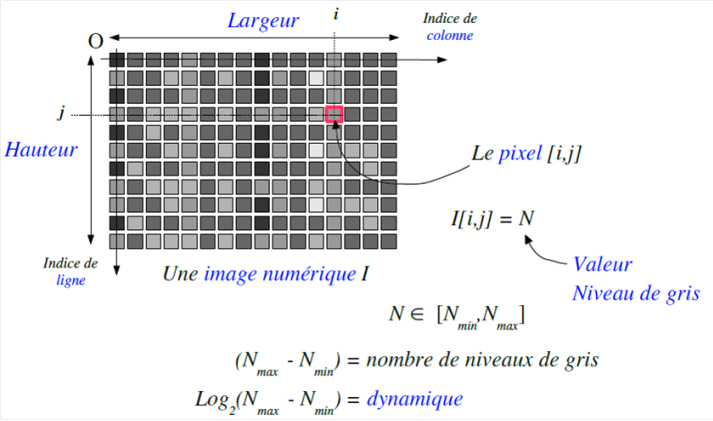
\includegraphics[width=0.7\textwidth]{Figures/pixel} 
	\caption{Image numérique au niveaux de gris: notion de pixel.}
\end{figure}


Un pixel $(i, j)$, ( i est l'indice de la ligne et j est l'indice de la colonne), possède une valeur $I(i, j)$ qui peut être un scalaire représentant la valeur du niveau de gris du pixel (dans le cas des images noir et blanc ou des images en niveaux de gris), ou un vecteur représentant les trois canaux de la couleur du pixel (dans le cas des images couleurs).\\

Ces images peuvent être regroupées en plusieurs catégories:



%-----------------------------------
%	SUBSECTION 1
%-----------------------------------

\subsubsection{Image à niveaux de gris}
 Les images à niveaux de gris sont composées de pixels de valeurs scalaires représentant la luminosité/intensité. En général ces valeurs des pixels sont  codés sur $n$ bits, ce qui lui confère des valeurs entières comprises entre 0 et $2^n-1$, 0 et 255 si $n = 8$. Dans ce cas, le pixel est codé sur un octet (nous disposerons ainsi de $2^8=256$ couleurs). La valeur 255 correspond au blanc, et la valeur 0 correspond au noir. Les valeurs intermédiaires correspondent à des niveaux de gris allant du noir au blanc.\\

La figure 1.1 ci-dessous montre une sous-matrice de $5 \times 5$ pixels extrait d’une image. Nous pouvons voir les valeurs qui composent la sous-matrice et les niveaux de gris qui permettent d’afficher l'image.

\begin{figure}[H]
	\centering
	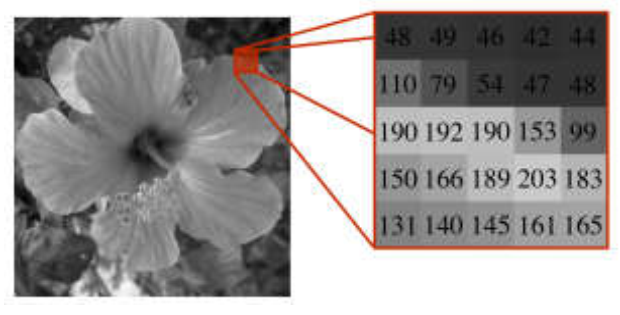
\includegraphics[width=0.4\textwidth]{Figures/gray} 
	\caption{Image à niveaux de gris.}
\end{figure}

\begin{figure}[H]
	\label{fig:tableRVB}
	\centering
	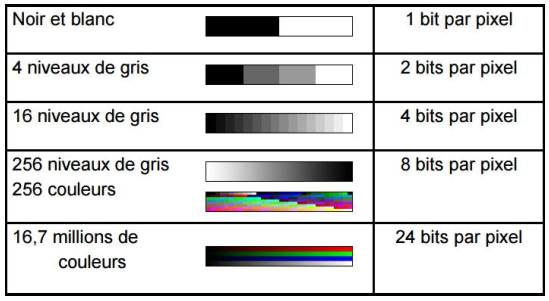
\includegraphics[width=0.65\textwidth]{Figures/tableRVB} % Include the image .png
	
	\caption{Représentation des pixels en fonction de nombre des bits.}
	
\end{figure}
%-----------------------------------
%	SUBSECTION 2
%-----------------------------------
\subsubsection{Image couleur}
Une image couleur est composée de pixels dont les valeurs sont en général multicomposantes. En effet, nous pouvons citer parmi les formats les plus utilisés pour représenter la valeur du pixel, le triplet (R,V, B) ou (R,G,B) où R, G et B sont respectivement les valeurs des composantes rouge, verte et bleu du pixel. Chaque composante du triplet est représentée par un entier variant entre 0
(absence de la composante) et 255 (intensité maximale). 

\begin{figure}[H]
	\centering
	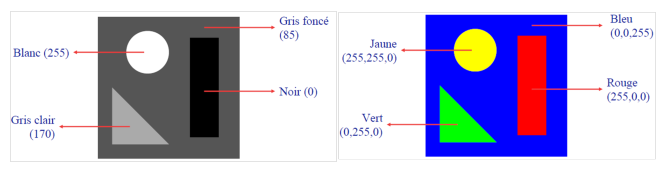
\includegraphics[width=0.6\textwidth]{Figures/grayvscol} 
	\caption{Image à niveaux de gris VS Image couleur.}
\end{figure}

Le triplet (0, 0, 0) correspond au noir, (255, 0, 0) au rouge, (255, 255, 0) au jaune et (255, 255, 255) au blanc.  Dans ce cas, le pixel est codé sur trois octets. Une image couleur RVB ou (RGB) possède trois composantes tandis qu'une image en niveaux de gris n’en possède qu’une seule. En d'autre termes, Une image couleur correspond à la synthèse additive de 3 images, rouge, vert et bleu. Chaque pixel est donc codé sur $3 \times n = 24 $ bits.

\begin{figure}[H]
	\centering
	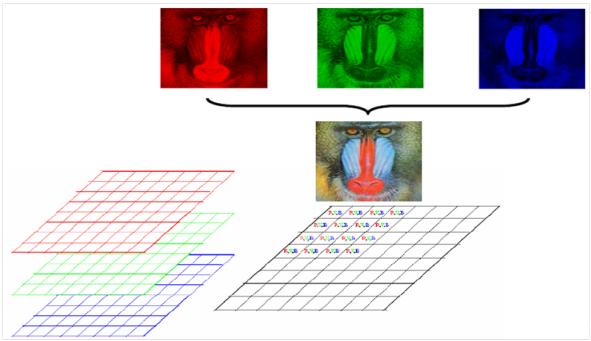
\includegraphics[width=0.6\textwidth]{Figures/rgb} 
	\caption{Image couleur dans l’espace RGB.}
\end{figure}

\subsection{Images vectorielles}
Les images vectorielles, contrairement aux images matricielles, contiennent les primitives de dessin (formes, position, couleurs...) des objets géométriques qu’elles représentent (segments de droite, polygones, arcs de cercles...). Ces images sont essentiellement utilisées pour réaliser des schémas ou des plans. Leur codage dépend directement du logiciel qui a permis de les créer. Ces images présentent deux avantages: elles occupent peu de place en mémoire et peuvent être facilement redimensionnées sans perte d'information (peuvent être agrandies à volonté sans perte de qualité).

\begin{figure}[H]
	\centering
	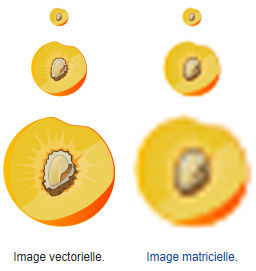
\includegraphics[width=0.3\textwidth]{Figures/vecteur} 
	\caption{Une image vectorielle: redimensionnable sans perte de qualité, contrairement à une image matricielle.}
\end{figure}



%-----------------------------------
%	SECTION 2
%-----------------------------------
\section{Formats d'images numériques}
Un format d'image est une représentation informatique, associée à des informations sur la façon dont l'image est codée et fournissant éventuellement des indications sur la manière de la décoder et de la manipuler. La plupart des formats sont composés d'un en-tête contenant des attributs (dimensions de l'image, type de codage, etc.), suivi des données de l'image. La structuration des attributs et des données diffère pour chaque format d'image [MM11].

\begin{table}[H]
	\centering
	\caption{Les différents formats des images matricielles.}
	\begin{tabular}{|l|l|l|l|}
		
		\hline
		\textbf{Format} & \textbf{Avantages} &
		\textbf{Inconvénients} & \textbf{Caractéristiques} \\
		\hline
		\makecell{JPEG : Joint\\
			Photographic\\
			Experts Group\\
			(extension
			.jpg)}
		& \makecell{Excellente\\
			compression\\
			avec la\\
			possibilité de\\
			sélectionner le\\
			taux} 
		& \makecell{Compression\\
			détruit la qualité.}
		&  \makecell{Le format le plus\\
			courant.\\
			Il ne supporte pas\\
			un fond transparent.\\
			Spécialement conçu\\
			pour les\\
			photographies.}   \\
		\hline
		
		\hline
		\makecell{GIF :
			Graphics\\
			Interchange\\
			Format\\
			(extension .gif)}
		& \makecell{Supporte\\
			l'animation et la\\
			transparence.\\
			Taux de\\
			compression\\
			élevé.} 
		& \makecell{Les couleurs\\
			sont définies sur\\
			une palette de\\
			256 couleurs.}
		&  \makecell{Utilisé généralement\\
			pour des photos de\\
			type dessin. Occupe\\
			peu d'espace disque.\\
			Presque tous les\\
			navigateurs peuvent\\
			le soutenir.}   \\
		\hline
		
		\hline
		\makecell{PNG : Portable\\
			Network\\
			Graphics\\
			(extension
			.png)}
		& \makecell{Emploie la\\
			compression\\
			sans perte de\\
			données,\\
			possibilité de\\
			transparence.} 
		& \makecell{Un peu plus\\
			lourd qu’un jpg\\
			donc il n’est pas\\
			très efficace pour\\
			les larges\\
			photographies.}
		&  \makecell{Format destiné à\\
			améliorer la\\
			limitation du\\
			format GIF. Appelé à\\
			devenir le futur\\
			standard internet.}   \\
		\hline
		
%	
%		\makecell{TIFF : Tagged\\
%			Image File\\
%			Format\\
%			(extension .tif)}
%		& \makecell{Il permet\\
%			d'obtenir une\\
%			image de très\\
%			bonne qualité,\\
%			possible\\
%			d’ajouter une\\
%			couche de\\
%			transparence.} 
%		& \makecell{Taille\\
%			volumineuse. Un\\
%			choix à éviter\\
%			pour le Web\\
%			puisqu'aucun\\
%			navigateur Web\\
%			ne le lit\\
%			directement.}
%		&  \makecell{le format le plus\\
%			couramment utilisé\\
%			pour stocker des\\
%			images.\\
%			Dédié pour les\\
%			professionnels\\
%			et pour l’impression\\
%			commerciale.}   \\
%		\hline
%		
%		\makecell{BMP : BitMaP\\
%			(extension
%			.bmp)}
%		& \makecell{Format natif de\\
%			windows. Pas de\\
%			perte de qualité.} 
%		& \makecell{Utilisable\\
%			uniquement sur\\
%			la plateforme\\ de
%			Microsoft. Taille\\
%			volumineuse.}
%		&  \makecell{Peu utilisé sur\\
%			le web.\\
%			Gère les palettes\\
%			pour les couleurs en\\
%			mode indexées.}   \\
%		\hline
	\end{tabular}
\end{table}


\begin{table}[H]
	\centering
	\caption{Les différents formats des images vectorielles.}
	\begin{tabular}{|l|l|l|l|}
		
		\hline
		\textbf{Format} & \textbf{Avantages} &
		\textbf{Inconvénients} & \textbf{Caractéristiques} \\
		\hline
		\makecell{AI : Adobe\\
			Illustrator \\(extension .ai)}
		 & \makecell{Reconnu par\\
			tous\\
			les logiciels\\
			graphiques.} & \makecell{Format propres\\ a
		Adobe Illustrator.}
		&  \makecell{Format développé\\
			par Adobe Systems.\\
			L'un des plus\\
			repandu pour la\\
			création de logotypes.}   \\
		\hline
		
		\makecell{EPS :
			Encapsulated\\
			Postscript\\
			(extension
			.eps)}
		& \makecell{Peut être\\
			visualisé et\\
			importé dans\\
			bon nombre de\\
			logiciels de\\
			dessins.} 
		& \makecell{Destinés qu'à\\
			l'impression.\\
			Fichier très\\
			lourd.}
		&  \makecell{EPS est un fichier PS\\
			qui comporte\\
			quelques restrictions\\
			supplémentaires. Le\\
			plus utilisé pour\\
			transférer une image\\
			ou une illustration.}   \\
		\hline
	
		\makecell{SVG : Scalable\\
			Vector\\
			Graphics\\
			(extension\\
			.svg)}
		& \makecell{Extensible car il\\
			est basé sur\\
			XML. Permet les\\
			animations et la\\
			transparence.} 
		& \makecell{Manque\\
			d'implémentation\\
			au sein de\\
			navigateurs\\
			(besoin d'un\\
			plugin).\\
			Production de\\
			code\\
			volumineux.}
		&  \makecell{Il est utilisé sur les\\
			mobiles, et souvent\\
			pour la création de\\
			"schémas,\\
			diagrammes ou\\
			cartes".}   \\
		\hline
%		
%		\hline
%		\makecell{SWF : Small\\
%			Web Format\\
%			(extension\\
%			.swf)}
%		& \makecell{Il est idéal pour\\
%			la publication\\
%			sur le web. Peut\\
%			contenir des\\
%			animations, mp3\\
%			et des JPEG.} 
%		& \makecell{Format\\
%			propriétaire.}
%		&  \makecell{Format spécifique à\\
%			Flash et accepté par\\
%			la majorité\\
%			des configurations\\
%			actuelles. Contrôler\\
%			par Adobe.}   \\
%		\hline
%		
%		\hline
%		\makecell{PICT : Picture\\
%			(extension\\
%			.pict)}
%		& \makecell{Créé par Apple\\
%			comme standard\\
%			pour ses\\
%			premiers\\
%			Macintosh.} 
%		& \makecell{Disponible\\
%			uniquement sur\\
%			les équipements\\
%			d'Apple.}
%		&  \makecell{Remplacé par d'autre\\
%			format en tant que\\
%			métaformat natif.}   \\
%		\hline
	\end{tabular}
	
\end{table}

%-----------------------------------
%	SECTION 3
%-----------------------------------
\section{Les caractéristiques d’une image numérique}
Les images numériques sont également définies par des propriétés appelées les caractéristiques globales, permettant généralement de mieux rendre compte de certaines propriétés visuelles de l'image, elles sont utilisées pour des traitements ultérieurs entrant dans le cadre d'applications telles que la détection d'objets ou la recherche d'images par le contenu par exemple.
Les caractéristiques globales d’une image numérique :

\subsection{Le Pixel}
Le pixel provient d’une abréviation de l’expression anglaise PICture Element (souvent abrégé px). C’est l'unité de base permettant de mesurer la
définition d'une image numérique matricielle.
L'ensemble de ces pixels est contenu dans un tableau à deux dimensions
constituant l'image finalement obtenue avec une couleur associée à chaque
pixel. Un pixel est si petit qu'on le voit à peine à l'œil nu, cela permet d'en
afficher beaucoup et d'avoir une image nette.

\subsection{La dimension}
La dimension ou la définition d’une image numérique, est le nombre total de pixels composant cette image. Il suffit de calculer le produit : largeur [px] * hauteur [px] pour déterminer la dimension. Par exemple : une image
avec une largeur = une hauteur = 8 pixels, La dimension = 8 * 8 = 64 pixels.

\begin{figure}[H]
	\centering
	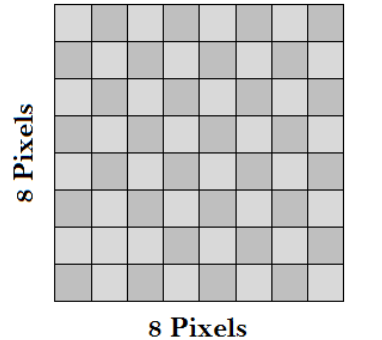
\includegraphics[width=0.3\textwidth]{Figures/dim} 
	\caption{La dimension d’une image.}
\end{figure}

\subsection{La résolution}
La résolution est la densité de l’image en pixels une fois reproduite,
mesurée en « ppi » (pixels per inch) ou en français « ppp » (pixels par pouce).
Elle décrit la clarté ou la finesse des détails d’une image matricielle. Plus le nombre de pixels par pouce est grand, plus la résolution est élevée.
Généralement, une image haute résolution produit une impression de
meilleure qualité.

\subsection{La couleur}
La couleur est la perception visuelle que nous avons des différentes
longueurs d’onde qui constituent la lumière visible. Cette partie du spectre
de la lumière s'étend du violet (4000 angströms) au rouge (7000 angströms),
les autres ne sont pas perçues.
Dans les systèmes de recherche d’image par le contenu, la couleur est
l'information visuelle la plus utilisée en raison de son invariance par rapport à l'échelle. 

Une couleur est généralement représentée par trois composantes. Ces composantes définissent un espace de couleurs. Il existe plusieurs espaces colorimétriques qui ont chacun certaines caractéristiques
intéressantes, le plus couramment utilisé est le système RGB.
\subsubsection{Espace des couleurs}
Une couleur est généralement représentée par trois composantes. Ces composantes définissent un espace des couleurs. On peut citer l'espace RVB, l'espace CIE (Commission Internationale de l'Eclairage) XYZ ou Yxy, ou encore l'espace Lab. Selon l'espace de couleurs choisi pour représenter une image couleur, le nuage des couleurs (c'est à dire l'ensemble des couleurs de l'image) n'aura pas la même répartition dans l'espace 3D.


\begin{figure}[H]
	\label{fig:espaceRVB}
	\centering
	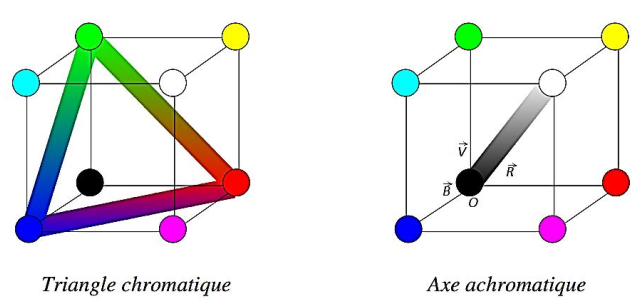
\includegraphics[width=0.65\textwidth]{Figures/espaceRVB} % Include the image .png
	\caption{Espace de couleur RVB.}
\end{figure}

Les espaces de couleurs classiques, tels que le RVB, CIE XYZ, ...etc, sont issus d'une approche purement physique, sans la prise en compte de données psychophysiques. Dans d'autre espaces de couleur, tels que l'espace Lab, l'approche physique est corrigée selon des données de la vision humaine.\\

De nombreuses méthodes de descriptions d'images proposent de caractériser la couleur dans certains espaces couleurs pour profiter des propriétés de ces derniers. La figure 1.9 montre les principaux espaces couleurs utilisés en indexation d’images [Ouhda19].
\begin{figure}[H]
	\label{fig:espaceCouleur}
	\centering
	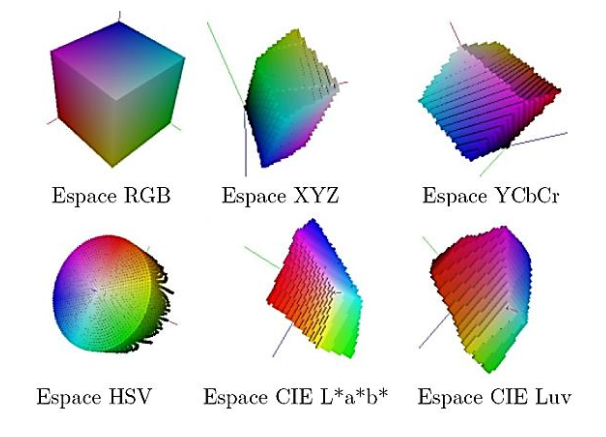
\includegraphics[width=0.45\textwidth]{Figures/espaceCouleur} % Include the image .png
	\caption{Les principaux espaces couleurs utilisés en indexation d'images.}
	
\end{figure}

On peut principalement citer :
\begin{itemize}
	\item \textbf{RGB} (Rouge, Vert, Bleu): est le plus utilisé car la plupart des images originelles sont codées dans cet espace couleur, ce qui ne nécessite pas de transformation inter espace couleur, donc facilement applicable.
	
	\item \textbf{HSV}: chaque composante représente respectivement la teinte, la saturation et la luminance.
	
	\item \textbf{YCbCr}: est utilisé dans les normes MPEG 1, 2 et 4, ses composantes sont décorrélées et de faibles dynamiques, ce qui permet de bons taux de compression.
	
	\item \textbf{L*a*b*} ou \textbf{CIE Luv}: sont des espaces couleurs perceptuellement uniformes. Ces espaces ont été créés dans le but de rendre plus homogène l’espace des couleurs et de
	permettre de mesurer uniformément les distances entre couleurs en tout point de l'espace. Deux couleurs proches dans ces espaces couleurs sont proches perceptuellement. Ces espaces sont grandement utilisés dans les systèmes de comparaison d'images.
\end{itemize}

\subsection{Contours et Textures}
Les contours représentent la frontière entre les objets de l’image, ou la
limite entre deux pixels dont les niveaux de gris représentent une différence significative [ZZ18]. Une texture se caractérise par la répétition d’un motif ou de quelques éléments. Plus précisément, la texture peut être vue comme un ensemble de pixels (niveaux de gris) spatialement agencés selon un certain nombre de relations spatiales, ainsi créant une région homogène [ZZ18]. On peut ainsi grâce à la texture faire la différence entre un coucher du soleil et une orange. Elle traduit donc l’aspect homogène d’une zone et peut être décrite selon ses propriétés spatiales et fréquentielles.\\

Dans le deuxième chapitre nous allons étudier la textures avec plus de détails.

\subsection{Luminance et Contraste}

\begin{itemize}
	\item \textbf{Luminance :}
	C’est le degré de luminosité des points de l’image. Elle est définie aussi comme étant le quotient de l’intensité lumineuse d’une surface par l’aire apparente de cette surface. Pour un observateur lointain, le mot luminance est substitué au mot brillance, qui correspond à l’éclat d’un objet.
	Dans le système international d'unités, la luminance s'exprime en candela par mètre carré, symbole ($cd/m^2$) [ZZ18].
	
	\item \textbf{Contraste :}
	C’est l’opposition marquée entre deux régions d’une image, plus
	précisément entre les régions sombres et les régions claires de cette image.
	Le contraste est défini en fonction des luminances de deux zones d’images (elle différencie les couleurs claires des couleurs foncées).
	Si $ L_1 $ et $ L_2 $ sont les degrés de luminosité respectivement de deux zones voisines $ A_1 $ et $ A_2 $ d’une image, le contraste $ C $ est défini par le rapport [ZZ18]:
	\begin{equation}
		 C = \frac{L_1 - L_2}{L_1 + L_2} 
	\end{equation}
\end{itemize}
 

 

\subsection{Le bruit}
Un bruit dans une image est considéré comme un phénomène de brusque
variation de l’intensité d’un pixel par rapport à ses voisins, il provient de l’éclairage des dispositifs optiques et électroniques du capteur.
Le bruit peut provenir de différentes causes :
\begin{itemize}
	\item Environnement lors de l'acquisition,
	\item Qualité du capteur,
	\item Qualité de l'échantillonnage.
	\item Ajouter par des techniques de traitement d'image numérique.
\end{itemize}


 
%-----------------------------------
%	SECTION 4
%-----------------------------------
\section{Traitement d'image numérique}
Le traitement d'image est l’ensemble d’opérations qui permettent
l’amélioration (filtrage, ...), la modification (rotation, symétrie) et l’extraction de l’information à partir des images numériques.
D'autre étapes sont nécessaires avant de commencer le traitement d’image
tel que :
\begin{itemize}
	\item L’acquisition et la numérisation de l’image par des dispositifs comme les scanners, les appareils photo qui permettent d’effectuer l’échantillonnage et la quantification d’une image.
	
	\item Il est facile d’effectuer les différentes opérations de traitement d’images grâce à des outils informatiques qui sont installés sur une unité centrale.
	
	\item Le stockage de l’image numérisée sur un support informatique (disque dur, CD-ROM, Clé USB, etc).
	
	\item L’affichage grâce à des dispositifs de visualisation qui permet l’affichage des images traités.
\end{itemize}

\begin{figure}[H]
	\centering
	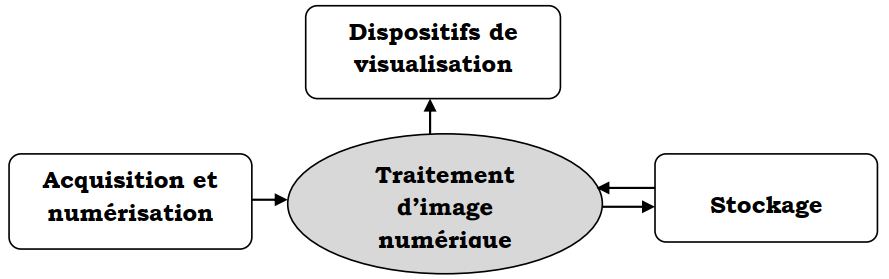
\includegraphics[width=0.6\textwidth]{Figures/tin} 
	\caption{Architecture d'un système de traitement d’image.}
\end{figure}

\subsection{Filtrage}
Les images numériques telles qu'elles sont acquises, sont très souvent
inexploitables pour le traitement d'images. Elles contiennent des signaux
bruités. Il est donc souvent nécessaire d'améliorer sa qualité. Deux types
d’améliorations des images sont possibles :

\begin{itemize}
	\item \textbf{Amélioration du rapport signal sur bruit :} La méthode la plus simple pour augmenter le rapport signal/bruit consiste à appliquer le principe des analyseurs multicanaux, c'est-à-dire effectuer plusieurs acquisitions de l’image (n par exemple) : ce qui revient à effectuer plusieurs sommations du signal. Le bruit n’apparaissant statistiquement jamais au même endroit, sera uniformément réparti, alors que le signal, apparaissant toujours au même endroit, sera amplifié d’un facteur racine carrée de n [ZZ18].
	
	Généralement, l'amélioration du rapport signal/bruit n’est pas suffisante pour obtenir une très bonne qualité, ce qui nécessite d’ajouter une deuxième amélioration que l’on appelle une opération de filtrage (ou lissage).
	
	\item \textbf{Amélioration par filtrage :}
	L'objectif avoué du filtrage est de réduire les variations d'intensité au sein de chaque région de l'image tout en respectant l'intégrité des scènes :
	les transitions entre régions homogènes, les éléments significatifs de l'image	doivent être préservés au mieux. Différentes méthodes de filtrage ont été développées suivant le type et l’intensité du bruit, ou les applications auxquelles on destine l'image.\\
	
\end{itemize}

Deux approches sont possibles dans la conception d’un filtre d’image.
La première consiste à construire un opérateur qui fonctionne de manière
linéaire et invariante dans le décalage. Ces filtres, au sens propre du terme, sont appelés filtres linéaires. L'alternative consiste à ne plus imposer au filtre de procéder de façon linéaire ou de façon invariante dans le décalage. On peut construire dans cette hypothèse un très grand nombre d’opérateurs que nous regroupons sous le terme de filtres non linéaires.

\subsubsection{Filtres linéaires}
Un filtre linéaire transforme un ensemble de données d'entrée en un
ensemble de données de sortie selon une opération mathématique appelée
convolution. Lorsqu'il s'agit de données numérisées comme dans le cas du
traitement d'image, la relation entre les valeurs des pixels de sortie et celle des pixels d'entrée est décrite par un tableau de nombres, généralement carré, appelé matrice de convolution. Le filtre local est dit linéaire si la valeur du nouveau pixel est une combinaison linéaire des valeurs des pixels du voisinage.

Un exemple des filtres linéaires est :
\paragraph{ $\bullet$ Filtre gaussien :}
L’expression gaussienne en deux dimensions est donnée par :
\begin{equation}
  G(x, y) = \frac{1}{2\pi \sigma^2} \exp(-\frac{(x-\mu)^2+(y-\mu)^2}{2 \sigma^2})
\end{equation}
Où x et y représentent les distances sur les deux axes, $\sigma$ et $\mu $ sont respectivement la moyenne et l’écart-type de la distribution gaussienne. L’intérêt de ce filtre est que l’on contrôle facilement le degré de filtrage à travers le paramètre $\sigma$. En numérique, le filtre est représenté mathématiquement par une matrice. La convolution qui permet de traiter l'image s'effectue de manière très simple.

Le pixel à traiter étant placé sur le centre du filtre, on multiplie les
coefficients du filtre par les valeurs des pixels correspondants et on calcule la moyenne qui est éventuellement pondérée. La discrétisation de ce filtre de la moyenne $\mu = 0$  et d’écart-type $\sigma = 0.6$. donne le masque suivant :

\begin{figure}[H]
	\centering
	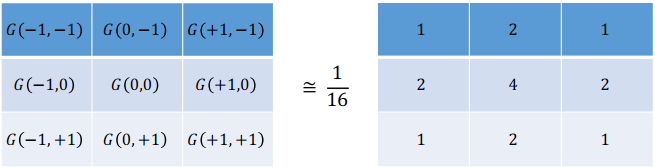
\includegraphics[width=0.5\textwidth]{Figures/gaussien} 
	\caption{Approximations discrètes de la distribution gaussienne de
		moyenne $\mu = 0$  et d’écart-type $\sigma = 0.6$.}
\end{figure}

\subsubsection{Filtres non linéaires}
Ils ont été développés pour régler l’insuffisance des filtres linéaires
surtout la mauvaise conservation des contours mais ils ont le défaut
d’imposer des déformations irréversibles à l’image. Leur principe est le même
que celui des filtres linéaires, il s’agit toujours d’utiliser des opérateurs
recherchant des valeurs de pixels extrémales au sein d’un voisinage.
Un exemple des filtres non linéaires est :

\paragraph{ $\bullet$ Filtre médian:}
Il appartient à la famille des filtres d’ordre. Le principe de ce filtre est de remplacer chaque valeur de pixel central par la valeur de pixel médiane observée dans leur voisinage. Cette valeur médiane permet d’éviter de procéder à des moyennes de valeurs de pixels de natures différentes. Son objectif est de réduire le bruit impulsionnel et préserver les contours.
\begin{figure}[H]
	\centering
	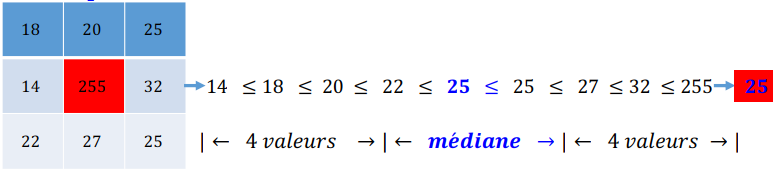
\includegraphics[width=0.6\textwidth]{Figures/median} 
	\caption{Principe du filtre médian.}
\end{figure}

\subsection{Détection de contour}
La détection de contour est une étape préliminaire à de nombreuses
applications de l'analyse d'images dans le but de repérer les points d’une
image numérique qui correspondent à un changement brutal de l’intensité
lumineuse. La détection des contours réduit de manière importante la
quantité de données et élimine les informations qu'on peut juger moins
pertinentes, tout en gardant les attributs importants de l'image.
Un contour se matérialise par une rupture d'intensité dans l'image
suivant une direction donnée. Ces changements d’intensités permettent de
décrire des variations importantes qui se traduisent par des discontinuités
dans la profondeur, dans l'orientation d'une surface, dans les propriétés
d'un matériau et dans l'éclairage d'une scène.\\

Il existe de nombreux filtres pour trouver les contours des objets. Ces filtres transforment l'image d'entrée en une image noire sauf aux points où un contour est détecté qui est marqué en blanc. Voici quelques exemples des filtres utilisés pour la détection de contour.

\begin{itemize}
	\item \textbf{Filtre de Prewitt :}
	Le filtre de Prewitt introduit un flou, chacune des deux matrices étant le produit du filtre dérivation dans la direction considérée par un filtre de flou	rectangulaire selon l'autre direction.
	
	\item \textbf{Filtre de Sobel :}
	La technique précédente est améliorée en remplaçant le filtre rectangulaire par un filtre triangulaire.
	
	\item \textbf{Filtre de Canny :}
	C’est un filtre de Sobel précédé par un lissage gaussien et suivi par un seuillage. 
	
\end{itemize}
\begin{figure}[H]
	\centering
	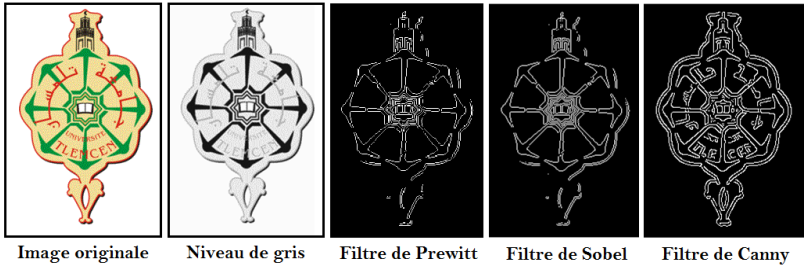
\includegraphics[width=0.5\textwidth]{Figures/conrour} 
	\caption{Détection de contour par les différents filtres.}
\end{figure}

\subsection{Segmentation}
La segmentation est une étape importante dans le traitement d'image numérique.
Elle consiste de partitionner l’ensemble des pixels de l'image entre eux selon des critères prédéfinis en différents régions connexes, qui constituent un pavage ou une partition de l'image, chaque région est supposée correspondre à un objet.
Lorsqu’un homme regarde une image, il peut séparer et reconnaitre les
objets situés dans cette image grâce à ces connaissances de haut niveau
(compréhension des objets et de la scène). Par exemple, si on travaille sur
une image d’un bureau, nous allons reconnaître facilement les ordinateurs,
les tables et les chaises. Contrairement, les machines informatiques ont
besoin des algorithmes bien développés pour faire la segmentation.
En effet, de nombreuses techniques ont été trouvées selon le type d’image
sur laquelle on travaille, et selon la nature des outils de segmentation
utilisés, certain sont plus performantes que d’autres, mais comme nous
allons le voir, les plus souvent sont destinées à un domaine particulier.
On considère principalement de nombreux types de segmentation, que l'on
peut regrouper en quatre classes principales [ZZ18] :
\begin{itemize}
	\item \textbf{Segmentation par régions : }consiste à caractériser les régions d’une image
	présentant un ensemble de pixels ayant des propriétés identiques
	différentes de celles des autres régions. On utilise généralement la
	méthode de "segmentation par croissance de régions" ou la méthode de
	"segmentation par division et rassemblement ".
	\item \textbf{Segmentation par détection de contour :} permet de borner les différentes
	régions par leurs frontières tout en utilisant la détection de discontinuité
	de ces trois composants : les points, les lignes et les contours.
	\item \textbf{Segmentation par seuillage :} cette opération utilise l’histogramme pour
	séparer et extraire les différentes régions de l’image (segmenter une image
	en plusieurs classes), à chaque pic de l’histogramme est associée une
	classe qui se caractérise par un intervalle de niveaux de gris.
	\item Segmentation fondée sur la combinaison entre les trois premières
	segmentations.
\end{itemize}
\begin{figure}[H]
	\centering
	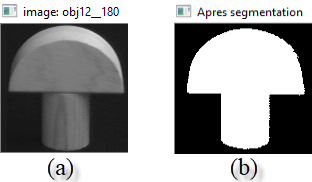
\includegraphics[width=0.5\textwidth]{Figures/segmentation.png} 
	\caption{Segmentation par seuillage de notre système.}
\end{figure}
%-----------------------------------
%	SECTION 5
%-----------------------------------
\section{Systèmes de recherche d'image par contenu (CBIR)}
Les chercheurs dans le domaine de la vision par ordinateur se posent le problème de l'indexation automatique des images par leur contenu, qui permet la recherche d'images par le
contenu (CBIR).\\

CBIR (Content Based Image Retrieval) est un système qui utilise des contenus{\tiny } visuels pour récupérer des images à partir d'une base de données d'images. Ce système est devenu indispensable parce qu'il peut effectivement surmonter les problèmes d'un TBIR (Text Based Image Retrieval). Dans le CBIR, le contenu visuel est extrait par plusieurs techniques:
histogramme, segmentation... Il est également décrit par le vecteur de caractéristiques multidimensionnel. En effet, Le CBIR diffère de la recherche d’information textuelle essentiellement par le fait que les bases de données d’images sont non-structurées, les images numériques n'étant que des matrices d'intensités de pixels, sans signification inhérente les unes par rapport aux autres. Donc avant même de commencer à faire des hypothèses sur le contenu de l'image, une des questions clé dans tout type de traitement d’image est l’extraction de l’information utile à partir de ces matrices de pixels car la performance du système de recherche d'images basées sur le contenu est principalement influencée par la qualité et la pertinence du vecteur de caractéristiques. \\

\subsection{Principe de la recherche d’images par contenu}
Les premiers moteurs de recherche d’images sont basés sur des textes et des mots-clés attribués à chaque image pour l'identifier, mais cette méthode a comme inconvénient que le résultat de recherche contient beaucoup des images qui ne sont pas nécessaires. Pour cela, les spécialistes ont travaillé sur une autre méthode, des systèmes adaptés pour l'approche « basé sur le contenu » (content-based, en Anglais) qui se propose de représenter les images en fonction de leur contenu.\\

Le principe général de la recherche d'image par le contenu comporte deux étapes:
\begin{itemize}
	\item  \textbf{Etape d'indexation (offline):} L'indexation est un ensemble de processus aboutissant à la
	construction d’un vecteur numérique appelé descripteur visuel de l’image.
	Dans cette étape hors ligne, le système commence	par le pré-traitement de l'image, c’est-à-dire l'extraction automatique des	attributs physique à partir des images de la base pour qu'ils doivent être compréhensible par la machine, cette opération peut être nommée "calcul de signature". Après la gestion et l'organisation de ces informations, le système stocke les signatures calculées dans une nouvelle base d'images appelée "base d'index" ou "base de signatures".
	
	\item \textbf{Etape de recherche (online):} La seconde phase, dite de recherche se déroule en ligne. L'utilisateur soumet une image comme requête. Le système calcule le vecteur descripteur (signature)  selon le même mode que lors de la première phase d'indexation. Ainsi, cette signature est comparé à l'ensemble des signatures préalablement stockés dans la base d'index pour en ramener les images les plus semblables à la requête ordonnées en fonction de la similarité à l’aide d’une mesure de distance..
\end{itemize}

\begin{figure}[H]
	    \label{fig:cbir_principe}
		\centering
		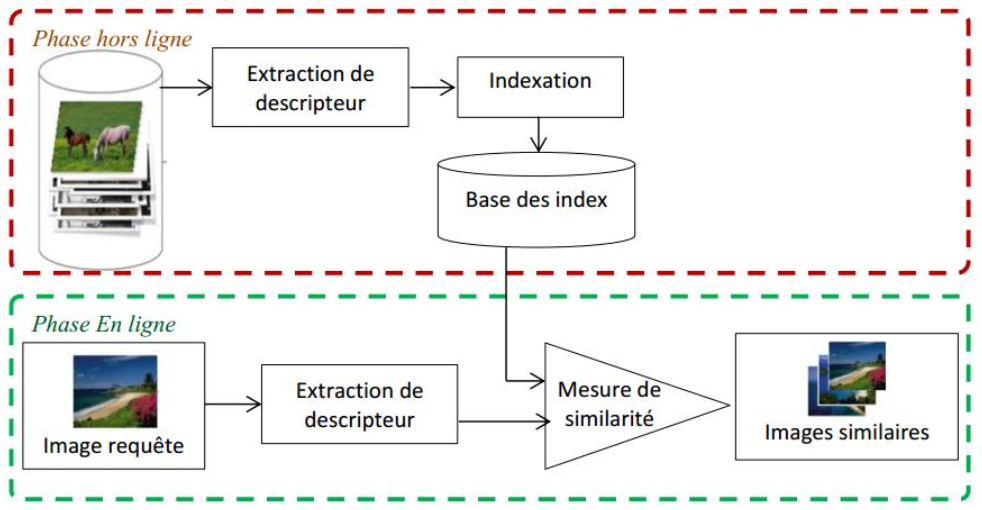
\includegraphics[width=0.7\textwidth]{Figures/cbir_principe} % Include the image .png
		\caption{ Architecture d'un système d'indexation et de recherche d'images.}
\end{figure}

Lors de la phase d'indexation, le calcul de descripteur consiste en l'extraction de caractéristiques visuelles des images telles que:
\begin{itemize}
	\item la texture (filtre de Gabor, transformée en ondelettes discrète…)
	\item la couleur (la segmentation, les points d’intérêts, les régions d’intérêts,
	histogramme de couleurs, histogrammes dans l'espace RGB ou dans TSV, …),
	\item les formes (descripteurs de Fourier, Les moments de Zernike, …),
	\item une combinaison de plusieurs de ces caractéristiques.
\end{itemize}

Ces caractéristiques sont dites de bas-niveau, car elles sont très proches du contenu signal (pixel), et ne véhiculent pas de sémantique particulière sur l'image.\\


\subsection{La base d’images}
La gestion de bases de données désigne la branche de l’informatique qui étudie le stockage et l’interrogation des données numériques. Une base de données informatique est donc un ensemble d’informations numériques stockées selon un modèle dans le but de les conserver, de les enrichir et de les interroger avec la garantie de l’intégrité de ces données [Jerome05]. Généralement, les systèmes de recherche d’images incluent deux bases différentes, la première collecte les images brutes, c’est-à-dire les images non traitées, et la deuxième gère les signatures des images indexées.\\

Ils existent plusieurs bases d’images sur Internet dont la plupart sont librement utilisées. Différentes par leur contenu, chaque base possède des images groupées en plusieurs classes bien définies où chaque image  n’appartient qu’à une seule classe. Généralement, les développeurs utilisent ces bases pour tester les algorithmes de recherche d’images mis en œuvre afin d’évaluer et valider leurs systèmes.\\

Cette section présente les bases d’images les plus utilisées dans le domaine de recherche d’image par le contenu :


\textbf{Columbia Object Image Library (COIL-100):}
C’est une Bibliothèque d’images de l’université de Columbia, elle a été créée en 1996. Cette base d’images est très connue pour la reconnaissance des objets. Il y a deux bases d’images COIL : COIL-20 qui contient des images en niveaux de gris prises à partir de 20 objets différents et COIL-100 qui contient des images en couleurs prises à partir de 100 objets différents. Les deux bases d’images consistent en des images prises à partir des objets 3D avec des positions différentes. La base COIL-100 a 7200 images en couleurs (100 objets x72 images/objet). Chaque image a une taille de 128x128 pixels. La base de Wang est disponible à l’adresse : \href{https://www1.cs.columbia.edu/CAVE/software/softlib/coil-100.php}{COIL-100}.

\begin{figure}[H]
	\centering
	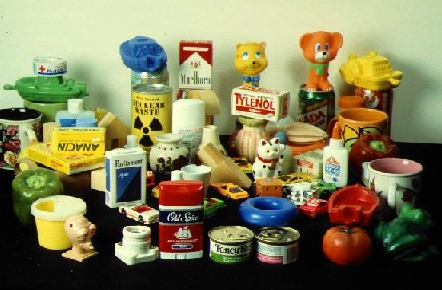
\includegraphics[width=0.5\textwidth]{coil} 
	\caption{Objets utilisés dans COIL-100.}
\end{figure}

\textbf{Corel-1000 - Wang:}
La base d’images de Wang est un sous-ensemble de la base d’images
Corel. Elle a été créée par le groupe du professeur Wang de l'université d'état de Pennsylvanie dans le but de faire des expériences de classification.
Cette base d’images contient 1000 images en couleurs. Ces images ont été divisées en 10 classes de 100 images. Les thèmes représentés par les 10 classes sont : monuments, plage, autobus, dinosaures, aliments, éléphants, fleurs, chevaux, montagnes et l’Afrique.
La base de Wang est disponible à l’adresse : \href{http://wang.ist.psu.edu/}{WANG}.
\begin{figure}[H]
	\centering
	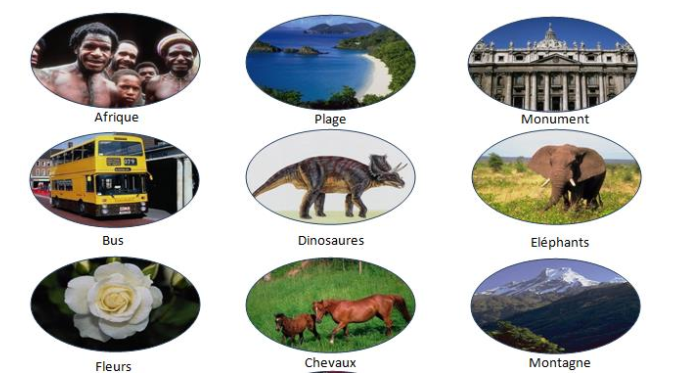
\includegraphics[width=0.6\textwidth]{wang} 
	\caption{Quelques images de la base d’image WANG.}
\end{figure}

\textbf{La base INRIA:}
Est un ensemble d’images photos personnelles de vacances. Cette base contient aussi des versions d’images changées à travers la rotation, le point de vue et d’illumination, flou, ...etc.

L’ensemble de données contient 500 groupes d’images, qui représentent une scène ou un objet distinct. La première image de chaque groupe est l’image de requête et les résultats corrects de récupération sont les autres images du groupe. La taille totale du corpus est : 1491 images au total : 500 questions et le reste ce sont les images de l’index. 

\begin{figure}[H]
	\centering
	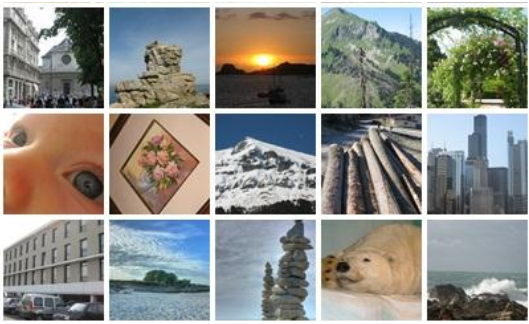
\includegraphics[width=0.6\textwidth]{inria} 
	\caption{Quelques images de la base d’image INRIA.}
\end{figure}


\subsection{Les requêtes}
La plupart des systèmes de recherche d’images disposent d'une interface graphique permettant aux utilisateurs d'effectuer une recherche par le biais d'une requête. L’utilisateur peut spécifier directement les attributs de bas niveau de l'image cible dans sa requête, interroger le système en esquissant un croquis, ou bien en présentant au système une image exemple de ce qu'il recherche.

Voici les quatre façons (types) pour faire une requête dans un système de recherche d'images :

\begin{enumerate}
	\item \textbf{Requête par description :}
	Dans cette méthode, l’utilisateur indique ce qu’il veut en termes de descripteur visuel, il décrit l’image qu’il souhaite obtenir en fonction de ces caractéristiques visuelles comme la couleur et la texture (par exemple, chercher une image contenant $40\%$ de bleu en haut, $20\%$ de vert en bas).
	Ces caractéristiques sont classées dans un répertoire dépend de moteur de
	recherche.
	
	\item \textbf{Requête par mots clés :}
	L’utilisateur exprime ses besoins en fournissant un ou plusieurs mots clés, qui peuvent être combinés à l'aide de connecteurs logiques tels que et, ou et non. Dans cette méthode, les systèmes se basent, en plus d'indexation par contenu, sur l’indexation textuelle manuelle d'image pour filtrer le résultat. Plusieurs moteurs de recherche d’images en ligne utilisent cette approche telle que Google et Yahoo, mais elle reste une façon de recherche fatigante surtout avec des bases d'images volumineuses [ZZ18].
	\begin{figure}[H]
		\centering
		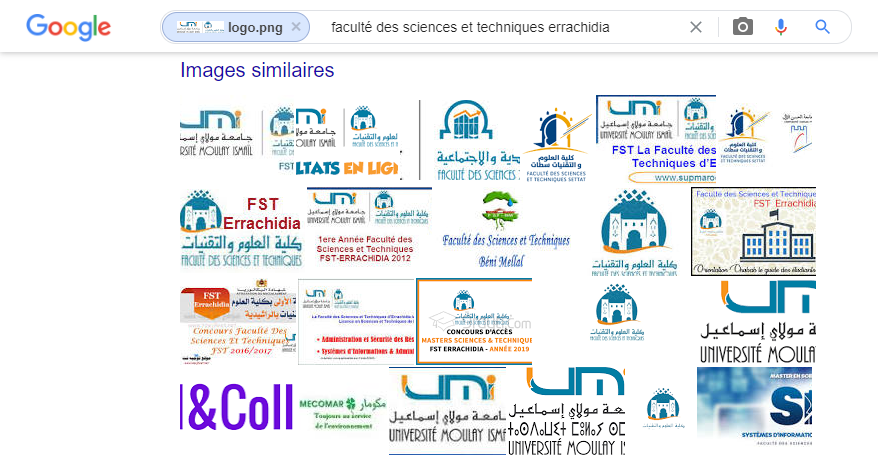
\includegraphics[width=0.6\textwidth]{fstelook} 
		\caption{Capture d’écran d’une recherche effectuée sur Google avec des mot-clés et une image, réalisée le 27/06/2020.}
	\end{figure}

	\item \textbf{Requête par esquisse :} Puisque les deux méthodes précédentes ont des désavantages, les chercheurs développent d'autres approches pour renforcer les moteurs
	de recherche d’images tel que la requête par esquisse ou bien par crayonnage. Dans cette approche, le système propose à l’utilisateur un ensemble d'outils de dessin et une palette de couleurs qui lui permet de spécifier sa requête en forme d’un sketch. Après, le système calcule les ressemblances entre le dessin et les images de sa base.
		\begin{figure}[H]
			\centering
			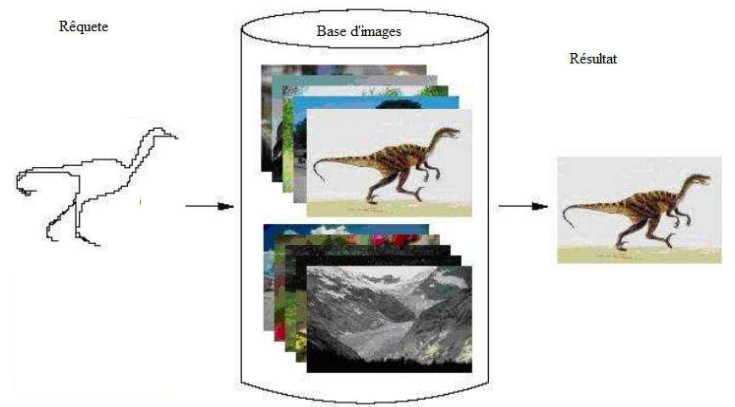
\includegraphics[width=0.6\textwidth]{croquis} 
			\caption{Exemple de requête par esquisse.}
		\end{figure}
	
	\item \textbf{Requête par image exemple :}
	Dans ce type de requête, il y a deux façons de commencer la
	recherche. La première consiste que l’utilisateur dispose d’une image de référence de ce qu’il cherche et la fournit au système comme un exemple.
	Dans la deuxième façon, le système montre à l’utilisateur quelques classes d’images, l’utilisateur sélectionne une classe et parcourt la liste d’images affichées par le système, puis il choisit une image de la liste comme étant une requête.
	Donc le système a besoin de comparer un exemple de même type (image) avec la base pour produire les items similaires. Cette méthode est simple, naturelle et ne nécessite pas de connaissances approfondies pour manipuler le système. Elle est donc bien adaptée à un utilisateur non spécialiste. C'est le type intégrer par notre système.
	
\end{enumerate}

\subsection{Mesures d’évaluation d’un système CBIR}
Une évaluation qui permet de mesurer la qualité d’un système de
recherche d’images est une étape nécessaire avant l’exécution de ce système. D’une façon générale, la recherche d’images par le contenu est une branche de la recherche d’informations, les objectives et les mesures d’évaluation du système qui ont été faits pour la recherche d’informations sont les mêmes
pour la recherche d’images. Par ailleurs, pour mesurer la performance d’un système, il faut qu'on dispose d'un ensemble d’images de test et d'une vérité terraine  (ground truth),
c'est-à-dire que nous savons préalablement quelles sont les images
appropriées à l'image requête dans la base d'images. Pour une évaluation significative il est important d'avoir un ensemble représentatif d'images requêtes. Ceci veut dire que l'ensemble des images requêtes doit être choisi d’une manière minutieuse [Khouloud09].
Dans l’exploitation de ces systèmes, les utilisateurs s’intéressent à deux objectifs principaux, un temps de réponse court et des résultats pertinents  du système, c'est-à-dire qu’il peut retrouver tous les images pertinentes et éliminer les images non pertinentes.


Dans cette section nous allons d’écrire les mesures les plus utilisées.

\subsubsection{Rappel et précision (en anglais : Recall and Precision)}

Dans les systèmes de recherche d’informations, afin de définir si une
information est pertinente ou non, on a besoin d’experts dans le domaine.
Dans les systèmes de recherche d’images, une image est pertinente pour une
requête si les deux images sont dans la même classe. C’est pourquoi dans
l’étape de préparation de la base d’images pour évaluer, on doit faire des
annotations. L’annotation est un processus qui permet aux utilisateurs de
choisir des mots clés correspondants à chaque image. Après l’annotation, on va classifier les images en classes appropriées. Si des images ne contiennent pas beaucoup d’objets, c’est facile de les classifier dans ces classes. Mais si les images contiennent beaucoup d’objets, la tâche de classification devient de plus en plus difficile. Dans ce cas-là, chaque image appartient à plusieurs classes .

\begin{itemize}
	\item \textbf{Le rappel :}
	Le rappel représente le rapport entre le nombre d’images pertinentes à la requête dans l’ensemble des images trouvées par le système et le nombre d’images pertinentes dans la base d’images.
	\begin{equation}
		R = \frac{| A \cap B|}{| A |} = \frac{\text{Nombre d'images pértinentes retrouvées}}{\text{Nombre total d'images pértinentes}}
	\end{equation}
	Où A l’ensemble des images résultat pertinentes pour une requête donnée et B l’ensemble des images résultat retournées par le système.
	
	\item \textbf{La précision :}
	La précision représente le rapport entre le nombre d’images pertinentes à la requête dans l’ensemble des images trouvées et le nombre d’images trouvées.
	
	\begin{equation}
	P = \frac{| A \cap B|}{| B |} = \frac{\text{Nombre d'images pértinentes retrouvées}}{\text{Nombre total d'images retrouvées}}
	\end{equation}
\end{itemize}

\begin{figure}[H]
	\centering
	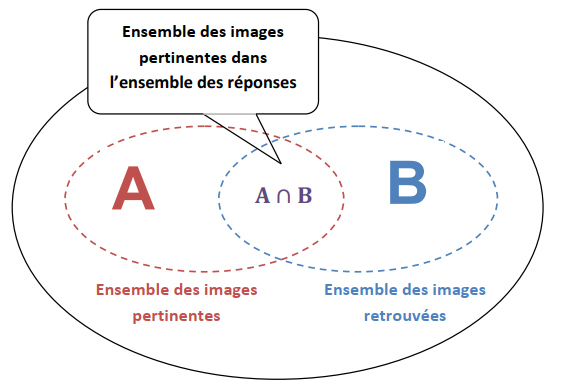
\includegraphics[width=0.4\textwidth]{recall} 
	\caption{ Le rappel et la précision pour une requête.}
\end{figure}

La précision et le rappel sont compris entre 0 et 1. Par exemple, si on utilise la base d’images de Wang qui contient 100 images par la classe " fleurs ", et le moteur de recherche retourne 8 images appropriées parmi 10 images trouvées, le rappel et la précision seront :
Le rappel = 8/100 = 0.08 ; la précision = 8/10 = 0.8.
Les deux métriques "rappel et précision" s’utilisent conjointement pour
l’évaluation des performances des systèmes de recherche. Les valeurs de ces deux métriques reflètent le point de vue de l’utilisateur (si le rappel est faible, une partie de l’information pertinente ne lui sera pas accessible, et si la précision est faible, l’utilisateur ne sera pas satisfait à cause de la forte concentration des informations non-pertinentes fournies dans les résultats).
Dans les deux cas, le système ne répond pas aux attentes des utilisateurs à retourner l’information utile et pertinente, et par la suite, il est nonperformant. Le cas idéal est d’avoir la valeur de précision et rappel
respectivement égale à un [Imane12].

\subsubsection{La courbe rappel/précision}
En pratique, le calcul d’une paire de valeurs (rappel et précision) ne
peut pas indiquer la performance du système. Donc il est nécessaire
d’utiliser plusieurs requêtes afin de donner une distribution de
rappel/précision sous forme d’une courbe, où chaque point de cette courbe
représente la précision moyenne calculée pour toutes les images
correspondant à ce niveau de rappel. Ce calcul statistique permet de suivre
la qualité du résultat en fonction du nombre d’images affichées par le
système en réponse à une requête.
La figure 1.22 donne un exemple de courbe de rappel et précision.
\begin{figure}[H]
	\centering
	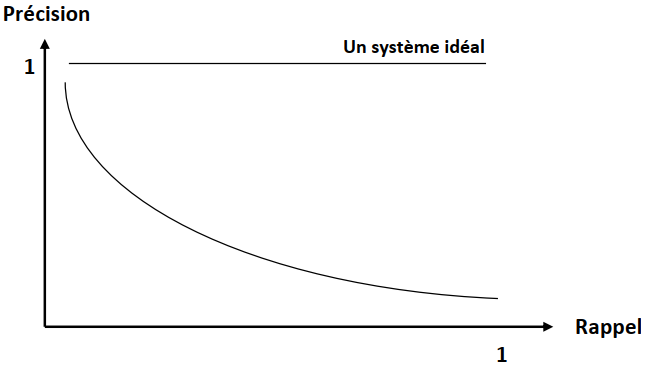
\includegraphics[width=0.4\textwidth]{courve} 
	\caption{Une courbe de rappel/précision.}
\end{figure}

Le rappel et la précision sont très utiles parce qu’ils nous permettent
d’évaluer quantitativement la qualité de la réponse globale. Mais ils ont ces quatre désavantages.
\begin{itemize}
	\item L’estimation de la valeur maximum de rappel exige de savoir toutes les connaissances de la base d’images. Quand la base d’images devient de plus en plus grande, ces connaissances ne sont pas disponibles, ce qui veut dire que l’évaluation n’est pas bien estimée.
	\item Le rappel et la précision sont reliés. Donc dans quelques cas, les deux mesures ne sont pas suffisantes. L’utilisation d’autres mesures qui combinent le rappel et précision pourrait être plus appropriée.
	%\item Ces mesures travaillent bien sur un ensemble de requêtes par lots. Cependant, les systèmes modernes ne travaillent pas dans ce mode.
	%\item Le rappel et la précision sont faciles à définir quand l’ordre des images est linéaire. Ces mesures ne sont pas appropriées pour les systèmes qui ont un ordre faible.
\end{itemize}

A cause de ces désavantages, d’autres mesures qui sont plus appropriées
doivent être utilisées comme :

\begin{itemize}
	\item \textbf{La moyenne harmonique ou F-mesure:} Mathématiquement, la moyenne 
	harmonique H est utilisée lorsqu'on
	veut déterminer un rapport moyen,
	dans un domaine où il existe des 
	liens de proportionnalité inverses.
	Dans notre cas, la moyenne harmonique
	combine le rappel et la précision en un
	nombre\\ réel compris entre 0 et 1 
	\begin{equation}
	    F = \frac{2}{\frac{1}{R}+\frac{1}{P}} = \frac{2\times R \times P}{R+P}
	\end{equation}
	Où :\\
	R : la valeur du rappel.  \space\space	P : la valeur de la précision.
	
	
	Si cette valeur vaut 0 ça veut dire
	qu’aucune image pertinente n’a été
	retrouvée. Si la valeur vaut 1, toutes
	les images pertinentes ont été
	retrouvées. De plus, cette mesure a 
	une valeur élevée quand le rappel et la
	précision sont élevés.
	
	\item\textbf{ La mesure E :}

	\begin{equation}
			 E = \frac{1+b^2}{\frac{b^2}{R}+\frac{1}{P}}
	\end{equation}
	
	Elle permet à l’utilisateur d’indiquer 
	s’il est intéressé par le rappel ou la précision.
	Si l’utilisateur choisit b > 1, ça veut dire qu’il s’intéresse plus à la précision.
	Et s’il choisit b < 1, ça veut dire qu’il donne la priorité au rappel plus qu’à la précision.    
\end{itemize}
		
		
%
%
%
%Une fois ces caractéristiques extraites, la comparaison consiste généralement à définir diverses distances entre ces caractéristiques, et de définir une mesure de similarité globale
%entre deux images. Au moyen de cette mesure de similarité et d'une image requête, on peut alors calculer l'ensemble des mesures de similarités entre cette image requête et l'ensemble des images de la base d'images. On peut alors ordonner les images de la base suivant leur score, et présenter le résultat à l'utilisateur, les images de plus grand score étant considérées comme les plus similaires.\\
%
%Ce genre de système ne nécessite pas forcément une image requête pour rechercher d'autres images. Par exemple, il est possible de rechercher des images plutôt bleues, ou alors de dessiner une forme et demander de chercher toutes les images qui possèdent un objet de forme similaire.
%
%
%
%Une des étapes essentielles en analyse d'images par le contenu est l'extraction d'une description de bas niveau de l’image. Cette description est une représentation numérique (analyse statistique, analyse quantitative, ...) des caractéristiques visuelles de l'image, généralement sous la forme d’un vecteur ou d’un ensemble de vecteurs.
%Cette description doit avoir deux caractéristiques importantes :
%\begin{itemize}
%	\item elle doit conserver suffisamment d’information pour être discriminante, c’est-à-dire différencier deux images avec un contenu visuel différent;
%	\item elle doit être la plus invariante possible (aux bruits; aux variations d’échelle; aux variations de contraste; aux déformations; etc) pour pouvoir généraliser le contenu visuel d’une image à une autre image qui n’est pas identique.
%\end{itemize}
%
%
%Nous présentons dans la suite les différentes familles de descripteurs.
%
%
%\subsection{Descripteur globaux et descripteurs locaux}
%On peut résumer l’ensemble des informations visuelles de l’image en un unique descripteur
%global, ou plusieurs descripteurs locaux caractérisant chacun une partie de l’image. Les
%techniques modernes en imagerie tendent à privilégier les descripteurs locaux aux globaux car
%les descripteurs locaux sont plus efficaces et ils permettent une recherche plus fine et
%absorbent mieux certaines variations.
%
%\subsubsection{Descripteurs globaux}
%Dans le cas de descripteurs globaux, un seule descripteur décrit la totalité de l’image, cela
%les rend robustes au bruit qui peut affecter le signal, les histogrammes de couleur et des
%niveaux de gris en sont des exemples classiques [Stricker 94]. De nombreux descripteurs
%globaux sont également basés sur la texture et la couleur. La couleur aussi fait partie des
%premières primitives visuelles utilisées. Le plus simple des descripteurs globaux basés sur la
%couleur consiste à construire l’histogramme des couleurs.
%L’inconvénient de ces descripteurs est qu’ils ne permettent pas de distinguer des parties de
%l’image, ils ne distinguent pas, par exemple, les objets dans l’image, sauf dans le cas où
%l’image ne contient qu’un seule objet sur un fond uni.
%
%\subsubsection{Descripteurs locaux}
%Les descripteurs locaux s’associent à une partie/région de l’image qu’on commence par
%détecter avant de calculer le descripteur, cette partie peut concerner un objet par exemple, la
%détection se fait indépendamment de la position dans l’image, ce qui assure l’invariance par
%translation, rotation, etc .
%
%Les descripteurs locaux sont de nos jours les caractéristiques visuelles les plus couramment
%utilisées en analyse d’image par le contenu. Ils permettent de décrire l’ensemble des
%informations visuelles d’une région de l’image en un descripteur (vecteur). La région
%d’extraction est appelée région d’intérêt et elle est généralement centrée sur un point d’intérêt
%Les descripteurs locaux ont une très bonne capacité de discrimination pour déterminer si
%deux régions sont similaires ou dissimilaires. Cela les rends particulièrement utiles en vision
%par ordinateur, notamment pour de la mise en correspondance de points d’intérêts. Ils sont
%utilisés en : odométrie visuelle [Nistér 04] ; reconstruction 3D [Mouragnon 06] ; détection
%d’objets [Lowe 99] ; recherche d’images par le contenu [Perronnin 10], [Negrel 14] ; etc.
%Dans le chapitre suivant, nous présentons un descripteur local basé sur la segmentation par
%k-means.
%
%\subsection{Combinaison des descripteurs}
%
%Les attributs: couleur, texture, forme décrivent les images par leur contenu visuel. La
%combinaison de ces attributs peut être mieux caractérisée le contenu. Il est donc intéressant de
%combiner ces différents attributs pour une recherche plus efficace et plus discriminante. Les
%problèmes qui se posent lors de la combinaison de ces différents attributs pour la recherche et
%l’indexation sont au moins de trois ordres :
%\begin{itemize}
%	\item L'espace de description : Le choix de l'espace de description consiste à rechercher les
%	attributs visuels significatifs de la base de données d'images, l'ensemble de ces
%	attributs étant représenté par un nuage de points dans un espace dimensionnel haut,
%	alors les vecteurs contiennent plusieurs attributs, un problème qui se pose est celui de
%	la dimension de l'espace de description. Ce problème est connu dans la communauté
%	des bases de données par la malédiction de la dimension, lorsque le nombre de
%	dimensions augmente, le volume de l'espace croît rapidement si bien que les données
%	se retrouvent « isolées » et deviennent éparses.
%	\item La mesure de la similarité : Il s'agit d'une étape essentielle dans tout système de
%	recherche. Dans le cas où les images sont décrites par différents attributs, une solution
%	classique pour mesurer la similarité est de calculer séparément les mesures de
%	similarité pour chaque attribut et de déduire ensuite une mesure composite de la
%	similarité globale entre les images. Cela suppose évidemment que les différents
%	attributs sont indexés séparément (avec des structures d'index séparées). Dans la base de données, il y a peu de méthodes qui utilisent plusieurs index pour structurer les
%	données. Une autre difficulté liée à la similitude est de déterminer comment combiner
%	plusieurs mesures souvent définies sur des domaines différents, avec des dynamiques
%	différentes, des degrés d'importance différents, surtout pour l'utilisateur, mais aussi de
%	natures différentes.
%	\item Structuration : la phase de construction d'une structure d'index est une étape utile dans
%	le cas où les données sont volumineuses et appartiennent à un grand espace de
%	description. Il s'agit de structurer les nuages de points relatifs aux descripteurs des
%	images et de les stocker efficacement dans une machine. Cette tâche de structuration
%	peut s'avérer difficile dans le cas où les données à structurer sont de nature hétérogène.
%	La difficulté réside dans le choix de la distance à utiliser pour structurer (mise en place
%	d'un index) et dans la standardisation des différents types de données.
%\end{itemize}
%
%

%----------------------------------------------------------------------------------------
%	SECTION 2
%----------------------------------------------------------------------------------------


\section{Conclusion}
Ce chapitre a fait l’état de l’art sans exhaustivité des différentes notions de base qui décrivent le domaine de traitement de l'image numérique et les systèmes de  recherche d'images par le contenu ainsi que les approches correspondantes. Nous avons abordé premièrement une brève définition sur l’image numérique et ces caractéristiques. Ensuite, nous avons étudié le principe de traitement d’image avec ces étapes tel que le filtrage et la segmentation. Aussi, nous avons défini brièvement le principe d’un système de recherche d’images par le contenu (CBIR) ainsi que l’architecture de fonctionnement. Ensuite, nous avons présenté les différentes bases d’images les plus utilisées, les types de requête et la représentation des images dans ces systèmes. A la fin de ce chapitre, nous avons aussi montré les mesures utilisées pour évaluer un CBIR comme le rappel et la précision.\\

Le chapitre suivant sera consacré à deux étapes fondamentales dans la
recherche d’images par le contenu. L’extraction d’attributs pour la création des vecteurs descripteurs (signatures) et la mesure de similarité entre une image requête et les images de la base d'index.


% Chapter Template

\chapter{Descripteurs d'Images \&  Mesures de Similarité} % Main chapter title

\label{Chapter2} % Change X to a consecutive number; for referencing this chapter elsewhere, use \ref{ChapterX}

%----------------------------------------------------------------------------------------
%	SECTION 1
%----------------------------------------------------------------------------------------

\section{Introduction}
Aujourd’hui avec le développement des systèmes multimédias, nous utilisons de plus en plus le contenu visuel comme support de communication dans différents domaines. En effet l’image et la vidéo numérique sont partie intégrante de tels systèmes par la densité et la richesse de leur contenu. La même image peut présenter plusieurs significations à différents niveaux : analyse, description, reconnaissance et interprétation. Dans notre domaine, le premier but de n’importe quel système de recherche d’images est de fournir des résultats totalement satisfaits pour l'utilisateur, ce qui nécessite d’utiliser les meilleures méthodes d’extraction de caractéristiques (Descripteurs) et les représenter d’une manière réduite afin d’atteindre un temps de réponse acceptable pour un système de recherche d'images. L'information obtenue dans cette étape d'extraction est une sorte de résumé des images de la base. La transformation est généralement gourmande en temps de calcul.\\

Dans ce chapitre, nous présentons les différents descripteurs utilisés dans les systèmes de recherche d'image par contenu et ensuite les mesures de similarité entre les images après la définition de leurs vecteurs descripteurs (signatures ou attributs).




%----------------------------------------------------------------------------------------
%	SECTION 2
%----------------------------------------------------------------------------------------

\section{Descripteurs d'image}
Le CBIR diffère de la recherche d’information textuelle essentiellement par le fait que les bases de données d’images sont non-structurées, les images numériques n’étant que des matrices d’intensités de pixels, sans signification inhérente les unes par rapport aux autres. Donc avant même de commencer à faire des hypothèses sur le contenu de l’image, une des questions clé dans tout type de traitement d’image est l’extraction de l'information utile à partir de ces matrices de pixels.\\

Une grande partie du choix des descripteurs employés et des techniques associées à leur extraction permet d’avoir des systèmes de recherche d’images performants et robustes.
\paragraph{Définition:}
Un descripteur est défini comme la connaissance utilisée pour caractériser l'information contenue dans les images
[Nguy09]. 

De nombreux descripteurs sont développés et utilisés dans les systèmes de recherche pour décrire les images. Ceux-ci peuvent être différenciés selon deux niveaux :

\begin{table}[H]
	\begin{center}
		\caption{Classification des descripteurs.}
		\begin{tabular}{|l|l|}
			\hline
			\multicolumn{1}{|c|}{\textbf{Les descripteurs bas niveau}}                                                                                       & \multicolumn{1}{c|}{\textbf{Les descripteurs haut niveau}}                                                                                                                                                                                                   \\ \hline
			\begin{tabular}[c]{@{}l@{}}Décrivent le contenu bas niveau de \\ l'image, principalement en termes \\ de couleur, texture et forme.\end{tabular} & \begin{tabular}[c]{@{}l@{}}Décrivent le contenu sémantique \\ de l'image, et sont principalement\\ des mots clès fournis par l'utilisateur \\ lors de l'indexation, car l'extraction\\  automatique est un problème non \\ résolu actuellement.\end{tabular} \\ \hline
		\end{tabular}
		
	\end{center}
\end{table}

Les études que nous allons réaliser portent principalement sur des descripteurs bas-niveau, par la mise en place des descripteurs couleur, texture et forme.\\  

L'extraction de descripteurs peut avoir deux méthodes différentes, les descripteurs globaux qui sont extraits à partir de l’image entière et les descripteurs locaux qui sont calculés d'une partie de l'image. Les descripteurs calculés sur toute l’image permettent de minimiser le temps de calculs, la taille de données nécessaires ainsi que le coût. Au contraire, les descripteurs locaux sont bien adaptés aux images manipulées, mais l’utilisation de cette méthode reste longue et coûteuse.

 
%----------------------------------------------------------------------------------------
%	SUBSECTION 1
%----------------------------------------------------------------------------------------
\subsection{Les descripteur de la couleur}
La couleur est l’information visuelle la plus utilisée dans les systèmes de recherche par le contenu. Ces valeurs tridimensionnelles font que son potentiel discriminatoire soit supérieur à la valeur en niveaux de gris des images. Mais la caractérisation de la couleur dans une image est une opération extrêmement complexe. En effet, cette donnée varie considérablement avec l’orientation des surfaces, le point de vue de la caméra et l’illumination (positions et longueur d'onde des sources lumineuses). En outre, la perception de la couleur par l'être humain est un processus complexe et subjectif [Ouhda19].

\begin{figure}[H]
	\label{fig:imageRVB}
	\centering
	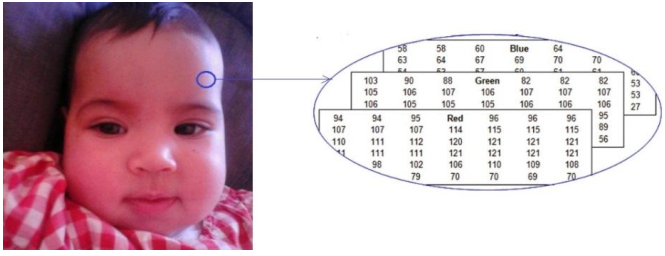
\includegraphics[width=0.65\textwidth]{Figures/imageRVB} % Include the image .png
	
	\caption{Image couleur dans l’espace RVB.}
	
\end{figure}

La couleur est devenue un attribut largement utilisé dans les systèmes opérationnels de recherche d'images par le contenu. Elle facilite l'identification et l'extraction d'un objet dans une scène [Zavi01]. Il semble que son efficacité à ce stade soit liée au fait que l'être humain peut distinguer des milliers de couleurs et seulement 24 niveaux de gris [Gonz02].\\

Généralement, la couleur est représentée par un espace colorimétrique de trois composantes. De nombreux travaux ont vu le jour quant à l’utilisation de la couleur pour la recherche d’images par le contenu. L’approche la plus courante dans la littérature est l’histogramme couleur.

\subsubsection{L'histogramme}
La plus grande majorité des systèmes de recherche d'images par le contenu se base sur la description des couleurs composant les images. L'histogramme des couleurs exprime la distribution statistique de celles-ci dans l'image.

Ce type d'histogramme est calculé typiquement sur un espace caractéristique quantifié. Chaque valeur de caractère dans l'histogramme représente donc un rang de couleur dans la palette. 

L'histogramme a été introduit pour la première fois en RIC (Recherche d'iformation par le contenu) par [Swain 91], depuis il est très utilisé à cause de sa simplicité de calcul, son invariante aux changements d'échelle et aux transformations géométriques.\\

\begin{figure}[H]
	\label{fig:hist}
	\centering
	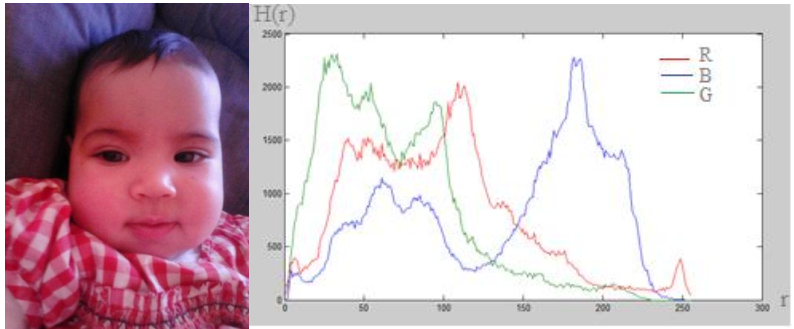
\includegraphics[width=0.65\textwidth]{Figures/hist} % Include the image .png
	\caption{Exemple d’histogramme d’une image couleur.}
\end{figure}

Les inconvénients majeurs de l'histogramme sont:
\begin{itemize}
	\item La perte de toute information spatiale dont la texture ou la forme. Par exemple un histogramme d'un tapis rouge peut être très proche de celui d'une porte rouge ou d'une voiture rouge.
	
	\item Ils sont de grandes tailles, donc par conséquent il est difficile de créer une indexation rapide et efficace en les utilisant tels qu'ils sont. 
	
	\item Ils sont sensibles à de petits changements de luminosité, ce qui est problématique pour comparer des images similaires, mais acquises dans des conditions différentes. 
	
	\item Ils sont inutilisables pour la comparaison partielle des images (objet particulier dans une image), puisque calculés globalement sur toute l’image.
	
\end{itemize}

\begin{figure}[H]
	\label{fig:samehist}
	\centering
	
\includegraphics[width=0.45\textwidth]{Figures/sameHist} % Include the image .png
	\caption{Deux images différentes de même histogramme.}
\end{figure}

Des méthodes alternatives ont été proposées pour augmenter l'efficacité de l'histogramme. Nous citons quelques-unes : 
\begin{itemize}
	\item les moments de la couleur [Stricker94], 
	\item les constantes de couleur [Flickner95],
	\item la signature couleur [Kender98], 
	\item les blobs [Chang97] et le vecteur cohérent de couleur [Pass97].
\end{itemize}


%----------------------------------------------------------------------------------------
%	subsubSECTION 2
%----------------------------------------------------------------------------------------
\subsubsection{Les moments de couleur}
Les moments de couleur on été utilisés dans plusieurs systèmes de recherche d’images par le contenu tel que QBIC (IBM's Query By Image Content). Mathématiquement, cette approche consiste à calculer l’espérance, l’équivalent d’une moyenne pondérée de tous les couleurs, puis la variance et les moments d’ordre 3 pour chaque composante couleur par les formules suivantes :

\begin{equation}
	\mu_i = \frac{1}{N} \sum_{j=1}^{N} p_{ij}
\end{equation}

\begin{equation}
	\sigma_i = \sqrt{\frac{1}{N} \sum_{j=1}^{N} (p_{ij}-\mu_i)^2}
\end{equation}

\begin{equation}
	s_i = \sqrt[3]{\frac{1}{N} \sum_{j=1}^{N} (p_{ij}-\mu_i)^3}
\end{equation}

Où $p_{ij}$ représente la valeur du pixel, $N$ représente le nombre total des pixels dans cette image.\\


La méthode d'histogramme utilise la distribution complète de la couleur. On doit stocker de nombreuses données. Au contraire, Les moments de couleur est une représentation compacte comparée aux autres descripteurs de couleur. Car seulement 9 valeurs (3 pour chaque composante chromatique) sont utilisées pour représenter le contenu d'une image. Dans [Stricker95], les auteurs ont prouvé que les méthodes des moments statistiques utilisées marchent plus vite et donnent des résultats meilleurs que les méthodes d’histogrammes.\\


%
%\subsubsection{Conclusion}
%L'information relative aux couleurs est particulièrement importante dans la caractérisation d’une image. Plusieurs études ont été menées pour trouver un critère de choix des descripteurs de couleurs pour l'indexation des images, mais aucune n'est pas suffisamment efficace. Ceci peut s’expliquer par le manque de subjectivité de cette information, les descripteurs couleur ne suffisent pas à indexer efficacement une image, ni à la chercher.
%
%Dans plusieurs domaines d’application, l’utilisation de descripteurs résumant l’information globale d’images couleurs n’offre pas toujours des résultats satisfaisants. Globalement, l’histogramme couleur reste le descripteur le plus utilisé vue qu'il garde un fort pouvoir de description. Bien qu’il ne contienne qu’une information partielle en raison de l’absence d’indication sur les caractéristiques spatiales.

%----------------------------------------------------------------------------------------
%	SUBSECTION 2
%----------------------------------------------------------------------------------------
\subsection{Descripteur de la texture}
Au même titre que la couleur, la texture est un  attribut visuel largement utilisé dans la recherche d’images par le contenu. Elle est également importante pour caractériser les motifs présents dans l’image. Elle permet de combler un vide que la couleur est incapable de faire, notamment lorsque les distributions de couleurs sont très proches. L'identification de la texture est une partie importante du système visuel humain, c'est un arrangement spatial de pixels, habituellement dans des modèles visuels homogènes que la couleur ne décrivent suffisamment. La modélisation et la description des textures sont un problème difficile. La texture est une caractéristique intuitive facile à reconnaître mais difficile à définir.

%-------------------------------------
%            SUBSUBSECTION
%-----------------------------------------
\subsubsection{Définitions}

D'après [Bimbo99], une définition formelle de la texture est quasiment impossible. De nombreuses définitions ont été proposées, mais aucune ne convient parfaitement aux différents types de textures rencontrées. Dans une définition couramment citée [Policarpo98], la texture est présentée comme une structure disposant de certaines propriétés spatiales homogènes et invariantes par translation. Cette définition stipule que la texture donne la même impression à l'observateur quelle que soit la position spatiale de la fenêtre à travers laquelle il observe cette texture. Par contre l'échelle d’observation doit être précisée. On peut le faire par exemple en précisant la taille de la fenêtre d’observation.\\

En générale, la notion de texture est liée à trois concepts principaux:
\begin{enumerate}
	\item Un certain ordre local qui se répète dans une région de taille assez grande,
	
	\item Cet ordre est défini par un arrangement structuré de ses constituants élémentaires,
	
	\item Ces constituants élémentaires représentent des entités uniformes qui se caractérisent par des dimensions semblables dans toute la région considérée.\\ 
	
\end{enumerate}

\begin{figure}[H]
	\label{fig:textures}
	\centering
	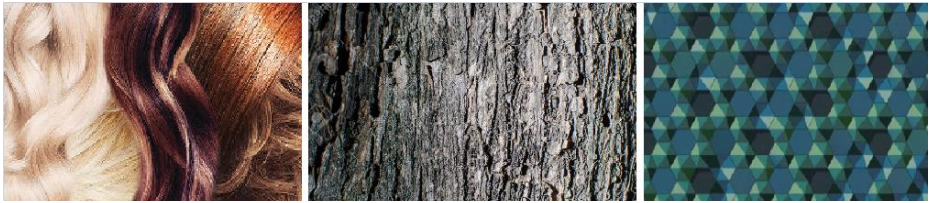
\includegraphics[width=0.65\textwidth]{Figures/textures} % Include the image .png
	\caption{Exemple des textures différentes.}
\end{figure}

\begin{description}
	\item[Définition 1:] 	
	D'une manière générale, la texture dans une image peut être définie comme un arrangement spatial de couleurs ou d'intensités dans une région de cette image [Linda01]. Elles peuvent consister en un placement structuré d’éléments mais peuvent aussi n’avoir aucun élément répétitif.
\end{description}

\begin{description}
	\item[Définition 2:] 	
	La texture peut être vue comme un ensemble de pixels (niveaux de gris) spatialement agencés selon un certain nombre de relations spatiales, ainsi créant une région homogène.
\end{description}

%-------------------------------------
%            SUBSUBSECTION
%-----------------------------------------
\subsubsection{Classifications de textures}
Il existe un grand nombre de textures. On peut les séparer en deux classes:
\begin{itemize}
	\item \textbf{Les textures structurées (macrotextures):} constituées par la répétition d’une primitive à intervalle régulier. On peut différencier dans cette classe les textures parfaitement périodiques (carrelage, damier, ...etc.), les textures dont la primitives subit des déformations ou des changements d'orientation (mur de briques, grains de café, ...etc.).
	
	\item \textbf{Les textures aléatoires (microtextures):} se distinguent en général par un aspect plus fin (sable, herbe, ...etc.). Contrairement aux textures de type structurel, les textures aléatoires ne comportent ni primitive isolable, ni fréquence de répétition. On ne peut donc pas extraire de ces textures une primitive qui se répète dans l’image mais plutôt un vecteur de paramètres statistiques homogènes à chaque texture.
\end{itemize}

Dans tous les cas, il est nécessaire d'extraire l'un ou plusieurs paramètres caractéristiques de cette texture. Nous désignerons ces paramètres sous le terme d’attributs texturaux (textural features).\\

Certains de ces paramètres correspondent à une propriété visuelle de la texture (comme la directionnalité ou la rugosité). D'autres correspondent à des propriétés purement mathématiques auxquelles il est difficile d'associer une qualification perceptive.
Un recensement ainsi qu'une classification des termes de description des textures employés par les principaux auteurs pourront être trouvés dans [Rao93] et [Lohse93].\\

De ces définitions et classifications, les recherches sur la modélisation des textures se sont portées sur la caractérisation de ces relations spatiales [Gueg07]. Quatre types d’approches se distinguent [Tuce98] [Zhan02] : 
les approches statistiques, les méthodes géométriques, les méthodes à base de modèles probabilistes et les méthodes fréquentielles. Ainsi, les attributs texturaux peuvent être obtenus à partir d’un ensemble assez vaste de différentes théories mathématiques, nous citons notamment :

\begin{table}[H]
	\begin{center}
		\caption{Classification des méthodes d’extraction de texture.}
		\begin{tabular}{ll}
			\hline
			\multicolumn{1}{|c|}{\textit{\textbf{Approche}}} & \multicolumn{1}{c|}{\textit{\textbf{Descripteur}}}  \\                             \hline 
			
			\multicolumn{1}{|c|}{\textbf{Statistiques}}      & \multicolumn{1}{l|}{\begin{tabular}[c]{@{}l@{}}- Matrice de longueur de plage\\ - Matrice de co-occurrence\\ - Méthode de différence de niveaux de gris\\ - Caractéristique de Tamura\\ - Méthode de dépendance spatiale des niveaux de gris\end{tabular}}  \\ \hline
			
			\multicolumn{1}{|c|}{\textbf{Fréquentielles}}    & \multicolumn{1}{l|}{\begin{tabular}[c]{@{}l@{}}- Transformée de Fourier discrète\\ - Filtre de Gabor\\ - Les ondelettes\end{tabular}}  \\ \hline
			
			\multicolumn{1}{|c|}{\textbf{\makecell{Méthodes à base\\ de modèle}}}    & \multicolumn{1}{l|}{\begin{tabular}[c]{@{}l@{}}- Décomposition de Wold\\ - Modèles Fractals\\ - Modèles AR (Autoregressive Models)\end{tabular}}  	\\ \hline
			
		\end{tabular}
		
	\end{center}
\end{table}


\subsubsection{Les matrices de co-occurrences (Mesures de Haralick)}
 En 1973, Haralick a proposé une méthode en se basant sur la matrice de co-occurrence de niveaux de gris [Haralick73], elle est probablement une méthode classiques et la plus célèbre pour l'analyser de la texture.
 
 La texture d'une image peut être interprétée comme la régularité d'apparition de couples de niveaux de gris selon une distance (pas $k=1, 2, 3, ...etc$) donnée dans l’image. La matrice de co-occurrences contient les fréquences spatiales relatives d’apparition des niveaux
 de gris selon quatre directions: $\theta = 0◦$,  $\theta =  \frac{\pi}{4} = 45◦$,  $\theta =  \frac{\pi}{2} = 90◦$,  $\theta =  3 \times \frac{\pi}{4} = 135◦$. Une matrice de co-occurrences est définie au moyen d’une relation entre deux pixels .\\

\begin{description}
	\item[Définition] La matrice de coocurrence $P_{d,\theta}=(P_{d,\theta}(i, j))_{1\leq i,j \leq Ng}$ est une matrice carrée de taille $Ng \times Ng$. Avec:
	\begin{itemize}
		\item Ng étant le nombre de niveaux de gris de l'image (256x256). Les indices de la matrice de co-occurrences sont
		donc les niveaux de gris de la texture étudiée.
		\item On réduit souvent a des tailles 8x8, 16x16 ou 32x32.
		\item L’élément $P_{d,\theta}(i, j)$de la matrice de cooccurrence définit la fréquence d'apparition des couples de niveaux de gris $i$ et $j$ pour les couples de pixels séparés par une distance $d$ dans la direction $\theta$.
		
		\begin{equation}
			P_{d,\theta}(i, j) = \sum_{x,y} 1_{ [I(x, y) = i \space \&\& \space  I(i + d, j + d) = v ]}
		\end{equation}
		Où: $ 1_{ [bool]} = 1 $ si $ bool = vrai $ sinon 0.
	\end{itemize} 
Pour obtenir de véritables fréquences relatives, il faut normaliser les éléments de la matrice en les divisant par le nombre total de paires de points élémentaires séparés par la distance d dans la direction dans toute l’image.
\end{description}

Alors on peut calculer plusieurs matrices, pour chaque distance (pas) et direction, mais avec un temps de calcul de ces matrices est assez long.

Soit l’image I définie par:

\begin{figure}[H]
	\label{fig:cooc}
	\centering
	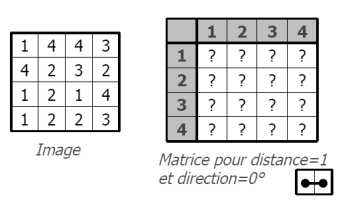
\includegraphics[width=0.65\textwidth]{Figures/cooc} % Include the image .png
	\caption{Matrice de co-occurrence.}
\end{figure}

On parcours l'image et pour chaque couple de pixels formé avec la distance et la direction données, on incrémente la matrice des co-occurrences de 1. Alors la matrice de co-occurrence (non normalisée) est:

\begin{figure}[H]
	\label{fig:cooc_nn}
	\centering
	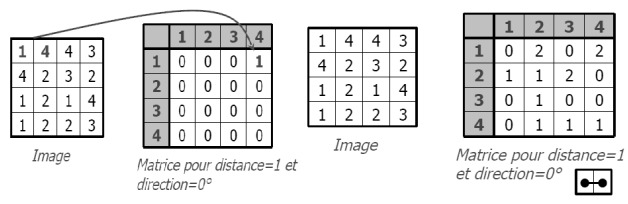
\includegraphics[width=0.8\textwidth]{Figures/cooc_non_norm} % Include the image .png
	\caption{Principe d'une atrice de co-occurrence:
	(a) et (c): image originale, (b): debut de calcul et (d): matrice de co-occurrence finale}
\end{figure}

Le 2 de la matrice de co-occurrence (ligne 1 et colonne 4) signifie que l’on trouve deux fois un pixel de valeur 1 de distance 1 et de direction
0 d’un pixel de valeur 4.\\


A partir de cette matrice de co-occurrence, il est possible de définir plusieurs descripteurs (Mesures de Haralick), tels que ceux répertoriés dans cette table:

\begin{table}[H]
	\centering
	\caption{Mesures de Haralick}
	\begin{tabular}{|c|c|c|}
		
		\hline
		\textbf{ Mesure} & \textbf{  Formulation} \\
		\hline
		Uniformité/Energie & \makecell{$E = \sum_{i=0}^{n}\sum_{j=0}^{n} P_{d,\theta}(i, j) $ }    \\
		\hline
		Entropie & \makecell{$En = -\sum_{i=0}^{n}\sum_{j=0}^{n} P_{d,\theta}(i, j) \log_2 (P_{d,\theta}(i, j)) $}    \\
		\hline
		Contraste & \makecell{$ C = \sum_{i=0}^{n}\sum_{j=0}^{n} P_{d,\theta}(i, j) (i-j)^2 $} \\
		\hline
	Moment inverse de différence & \makecell{$ M = \frac{1}{1+(i-j)^2} \sum_{i=0}^{n}\sum_{j=0}^{n} P_{d,\theta}(i, j)  $}\\
	     \hline
	\end{tabular}

\end{table}
 
 
\subsubsection{Transformée en ondelettes}
 Le terme " ondelette " en anglais (wavelet) a été utilisé pour la première fois en 1984 par J. Morlet et A. Grossmann pour résoudre des problèmes de traitement des signaux pour la prospection pétrolière. La transformée en ondelettes est à la base de nombreuses analyses de texture, telles que les filtres de Haar [Ganesan07].
 
 Une ondelette est une fonction à la base de la décomposition en ondelettes, décomposition similaire à la transformée de Fourier à court terme. La transformée en ondelettes consiste à décomposer un signal par une cascade de filtres pour générer une famille d'ondelettes appelées les ondelettes filles, obtenues par la translation et la dilatation d’une fonction mère. Chaque ondelette à une certaine fréquence pendant un temps limité, de la même façon que les notes de musique. La formule suivante présente une ondelette fille :
\begin{equation}
	\psi_{a,b}(t) = \frac{1}{\sqrt{a}}\psi(\frac{t-b}{a})
\end{equation}

Le paramètre $a$ est le facteur d’échelle, il détermine la dilatation de l'atome de base (ondelette fille). Le paramètre b est le facteur de translation, il permet de translater l'atome de base à gauche ou à droite. Le paramètre $ \frac{1}{\sqrt{a}} $ est un facteur de normalisation à travers les différentes échelles.\\

La transformée en ondelettes est un outil mathématique récent qui décompose un signal en fréquences en conservant une localisation spatiale. Le signal de départ est projeté sur un ensemble de fonctions de base qui varient en fréquence et en espace. Ces fonctions de base s’adaptent aux fréquences du signal à analyser. Cette transformation permet donc d’avoir une localisation en temps et en fréquence du signal analysé. La transformation en ondelettes continue est définie par :

\begin{equation}
	 F(a,b) = {\int }f\left(t\right) \psi_{a,b}^*(t) dt  
\end{equation}

Où, $ \psi_{a,b}^*(t) $ est la fonction de base d’ondelette. L’étoile «*» représente le complexe conjugué.

À partir de la transformée en ondelettes on peut extraire des attributs de différents types et à différents niveaux de résolution. L'image d'approximation donne des informations sur les régions qui composent l'image, d'une résolution fine à une résolution grossière. Les images de
détails donnent des informations horizontales, verticales et diagonales sur l'image [Jerome05]. Donc les ondelettes permettent de caractériser la texture en décrivant les primitives et les règles d'arrangement qui les relient.\\

L’approche continue des ondelettes pour un signal 2D est trop complexe pour être applicable
rapidement sur des images. Pour résoudre ce problème, Mallat considère l'analyse en ondelettes comme une décomposition du signal par une cascade de filtres, en utilisant une
paire de filtres pour chaque niveau de résolution (un filtre passe-haut et un filtre passe-bas) [Mallat89]. Il propose ainsi la DWT (Discrete Wavelet Transform) qui permet d'obtenir une transformée rapide. Le choix de l'ondelette mère est alors remplacé par le choix du filtre. Pour calculer une transformée en ondelettes, on n'a alors besoin que des deux filtres : au lieu de calculer le produit scalaire de l'ondelette avec le signal, on réalise un produit de convolution du signal avec ces filtres.\\

Une des transformées en ondelettes les plus couramment employées en analyse d'images est la
transformée de Haar, mais d'autres ondelettes sont aussi largement exploitées [Vailaya01]. Les filtres de Haar sont fréquemment employés en apprentissage pour obtenir la description d'un objet (comme un visage ou une personne). Pour avoir plus d'information sur les fondements mathématiques de la transformée en ondelettes, le lecteur peut se référer au livre [Vailaya01]. Comme pour la transformée de Fourier, une présentation plus pédagogique et plus historique des ondelettes peut également être trouvée
dans [Hubbard95].

\subsubsection{Transformée de Fourier discrète}
Extraire des informations fréquentielles d’une image est l’un des buts de l’utilisation de la
transformée de Fourier. Ainsi, nous pouvons extraire des attributs de texture à l’aide de la
transformée de Fourier comme par exemple l’énergie calculée dans une couronne ou bien en
fonction de certaines directions.\\

La transformée de Fourier discrète permet d’appliquer la transformée de Fourier aux signaux
numériques. Pour toute série numérique $s(n)$ à $N$ éléments, sa transformée de Fourier discrète
$S(k)$ est définie par :

\begin{equation}
	S(k) =  \sum_{n=0}^{N-1} s(n) \exp(-2i\pi k\frac{n}{N})
\end{equation}

En deux dimensions, cette équation devient :

\begin{equation}
S(k, l) =  \sum_{n=0}^{N-1} \sum_{m=0}^{M-1} s(n, m) \exp(-2i\pi k\frac{n}{N}) \exp(-2i\pi l\frac{m}{M})
\end{equation}

Le domaine des fréquences est alors divisé en : Anneaux, ou en secteurs angulaires et l’énergie calculée dans ces régions définit alors une caractérisation de la texture. Toutefois le principal problème de la transformée de Fourier est son manque de résolution spatiale. Cela signifie simplement que si nous sommes effectivement capables de détecter toutes les fréquences qui apparaissent dans un signal, nous sommes en revanche incapables de déterminer à quel moment elles se produisent dans le signal. Car si nous sommes en mesure d’interpréter le module de la transformée, il en est tout autrement de la phase qui est difficile à analyser. Ainsi il existe une transformée de Fourier plus locale donnant des informations mieux localisées appelée « Transformée de Fourier à fenêtre glissante » [Jerome05].

\subsubsection{Les filtres de Gabor}

Les filtres de Gabor sont largement utilisés en indexation, pour la description de la texture.
Introduit par Gabor [Gabor46], ces filtres ont été largement utilisés [Chawki16] à la fois comme fonctions de décomposition en ondelettes et comme outils d'analyse texturale [Andaloussi10]. Ces filtres peuvent prendre en compte l'orientation, l'échelle et la localisation des frontières, qui peuvent être utilisés pour caractériser la texture. Les filtres de Gabor sont des filtres passe bande, leur forme générale résulte de la multiplication d’une fonction de forme d'enveloppe gaussienne avec une fonction sinusoïdale complexe [ElAsnaoui17].\\

Les filtres de Gabor sont largement utilisés aujourd’hui pour modéliser la réponse du système visuel humain. En effet, ce dernier décompose les images texturées en un nombre important d'images filtrées dont chacune contient les variations d'intensité à travers une bande de fréquence et une orientation bien déterminées [Partio02]. En effet, Marcelaje [Marcelaje80] a montré que les cellules du cortex humain pouvaient être modélisées par des fonctions de Gabor à une dimension. Cette décomposition a été utilisée par Manjunath [Manjunathi96] pour des indexations par les textures.\\

Les filtres de Gabor permettent une bonne résolution spatiale à haute fréquence et une bonne résolution harmonique sans grande précision spatiale à basse fréquence [Mercier01]. Sommairement, les paramètres de texture sont déterminés en calculant la moyenne et l’écart type des niveaux de gris de l’image filtrée par le filtre de Gabor. En fait, ce n’est pas une seule valeur de moyenne et d’écart type qui sera calculée, mais plutôt un ensemble de valeurs égal au nombre d’échelles multiplié par le nombre d’orientations utilisées. Nous aurons donc ce qui est parfois appelé la banque de filtre de Gabor. Mathématiquement, toutes les valeurs des moyennes et d’écarts type calculées seront regroupées dans un seul vecteur descripteur. \\

Un filtre de Gabor 2D est le produit d'une gaussienne elliptique dans toute rotation et un exponentiel complexe représentant une onde plane sinusoïdale. Nous rappelons que, dans le domaine spatial, la fonction de Gabor bidimensionnelle est une somme de deux fonctions sinusoïdales, l'une paire et réelle, l'autre impaire et imaginaire, modulée par une enveloppe gaussienne. Une fonction Gabor 2D $g(x, y)$ et sa transformée de Fourier $G(u, v)$ s'écrivent comme suit [Manjunathi96]:



\begin{equation}
	g(x, y) = \frac{1}{2\pi \sigma_x \sigma_y} \exp\left[-\frac{1}{2} (\frac{x^2}{\sigma_x^2} + \frac{y^2}{\sigma_y^2}) + 2\pi j W_x\right]
\end{equation}

\begin{equation}
	g_{mn}(x, y) = a^{-m} \exp\left[-\frac{1}{2} (\frac{(u-W)^2}{\sigma_u^2} + \frac{v^2}{\sigma_v^2})\right] 
\end{equation}


 avec : $\sigma_u = \frac{1}{2\pi \sigma_x } $ et  $ \sigma_v = \frac{1}{2\pi  \sigma_y} $. \\
 
 Un ensemble de fonctions similaires peut être générées à partir de la dilatation et la rotation de la fonction Gabor $g(x, y)$ :
 

\begin{equation}
 	G(u, v) = a^{-m} g(x', y')
\end{equation}


 où : $a \ge 1 $, $x' = a^{-m} ( x \cos(\theta) + y \sin(\theta) )$,  $y' = a^{-m} ( -x \cos(\theta) + y \sin(\theta) )$ , $\theta = \frac{n\pi}{K}$ et $m,n$ sont des entiers et indiquent l'échelle et l’orientation des ondelettes respectivement avec $m = 0,1,..., M-1 $,  $n=0,1,..., N-1$, et $K$ est le nombre d'orientations. Le facteur d’échelle $ a^{-m} $ vise à assurer que l'énergie est indépendante de $m$. Les paramètres $W$ et $\theta$ représentent la fréquence et l'orientation du signal sinusoïdal et constituent le paramètre de l'espace du filtre de Gabor.\\

\begin{figure}[H]
	\label{fig:gaborFig}
	\centering
	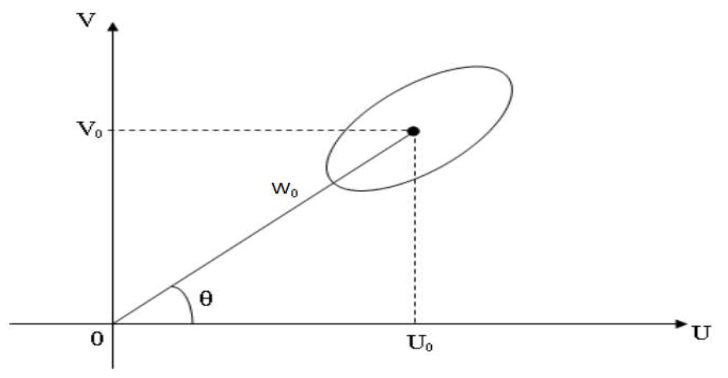
\includegraphics[width=0.65\textwidth]{Figures/gaborFig} % Include the image .png
	
	\caption{Contour à mi-niveau de la réponse en fréquence d’un filtre de Gabor 2D de fréquence centrale $W_0$ et d’orientation $\theta$.}
\end{figure}

L'utilisation des filtres de Gabor permet d'extraire de l'image considérée des informations pertinentes, à la fois en espace et en fréquence. Ils peuvent capturer le spectre de fréquence d'une image, en amplitude zt en phase. Ces filtres sont toujours utilisés par bancs dans lesquels chacun des filtres est réglé à une orientation et une fréquence précise. Les recherches conduites dans la littérature montrent que les fonctions de Gabor simulent de manière convenable le système visuel humain en reconnaissance des textures; le système visuel étant considéré comme un ensemble de canaux de filtrage dans le domaine fréquentiel.
 \begin{figure}[H]
 	\label{fig:gabor49}
 	\centering
 	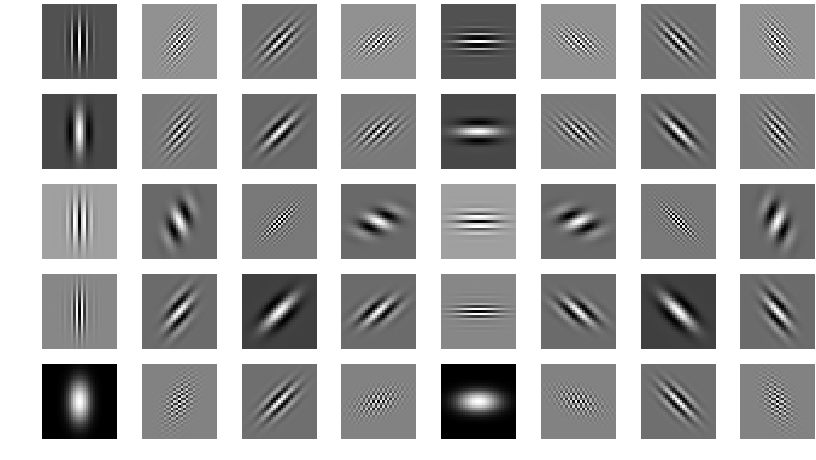
\includegraphics[width=0.65\textwidth]{Figures/gabor49} % Include the image .png
 	
 	\caption{Exemple du module des filtres de Gabor dans le domaine spatial.}
 	
 \end{figure}
 
 
%\subsubsection{Conclusion}
%
%Au même titre que l'information relative aux couleurs, Les attributs texturaux sont des attributs très importants pour la description de l'image et la reconnaissance de ses objets, cependant elles ne suffisent pas pour une bonne représentation du contenu de l'image, un inconvénient qui nécessite un autre attribut essentiel qui est celui de la forme.\\
%
%Dans la suite nous allons introduire cet attribut et les différentes approches utilisées pour
%l'extraire.

\subsection{Descripteur de forme}
Comme c'était le cas pour la texture, l'information de la forme est complémentaire de celle de la couleur pour la description de l'image.  Si l'être humain est particulièrement sensible à l'attribut de couleur pour distinguer les objets, pour certains types d'ambiguïté cela n'est pas suffisant et l'on a besoin de l'attribut de forme. La forme est généralement une description très riche d’un objet. Elle permet de détecter un objet sur une image plutôt que l’image elle-même. L’extraction d’attribut géométrique a été l’objet de la recherche d’images par le contenu ces dernières années.\\

La forme est un descripteur très important dans l'indexation des images. Elle est utilisée pour décrire la structure géométrique générique du contenu visuel. Généralement, les descripteurs de formes se divisent en deux catégories: 
\begin{itemize}
	\item les méthodes régions s'appuient sur la forme entière (règion). 
	\item les méthodes régions s'appuient sur le contour.
\end{itemize}
On peut ensuite distinguer deux familles pour chacune de ces catégories, une famille qui considère les objets comme une seule partie, et celle qui décrit les objets en les considérant comme un assemblage de sous parties. Une segmentation des objets est généralement utilisée avant l'extraction des attributs.\\

Les techniques d’extraction de forme par régions font référence aux moments invariants et sont utilisés pour caractériser l’intégralité de la forme d’une région. Ces attributs sont robustes aux transformations géométriques comme la translation, la rotation et le changement d’échelle [ElAsnaoui17]. La seconde approche fait classiquement référence aux descripteurs de Fourier et porte sur une caractérisation des contours de la forme. Ils ne peuvent pas détecter la structure interne de la forme puisqu’ils sont basés sur les contours uniquement. En outre, ces méthodes ne sont pas adaptées aux formes disjointes ou creuses, qui est le cas des symboles graphiques, car l’information sur le contour n’est pas disponible. Par conséquent, elles sont limitées à un certains types d’applications [Tabb06].

\begin{figure}[H]
	\label{fig:forme}
	\centering
	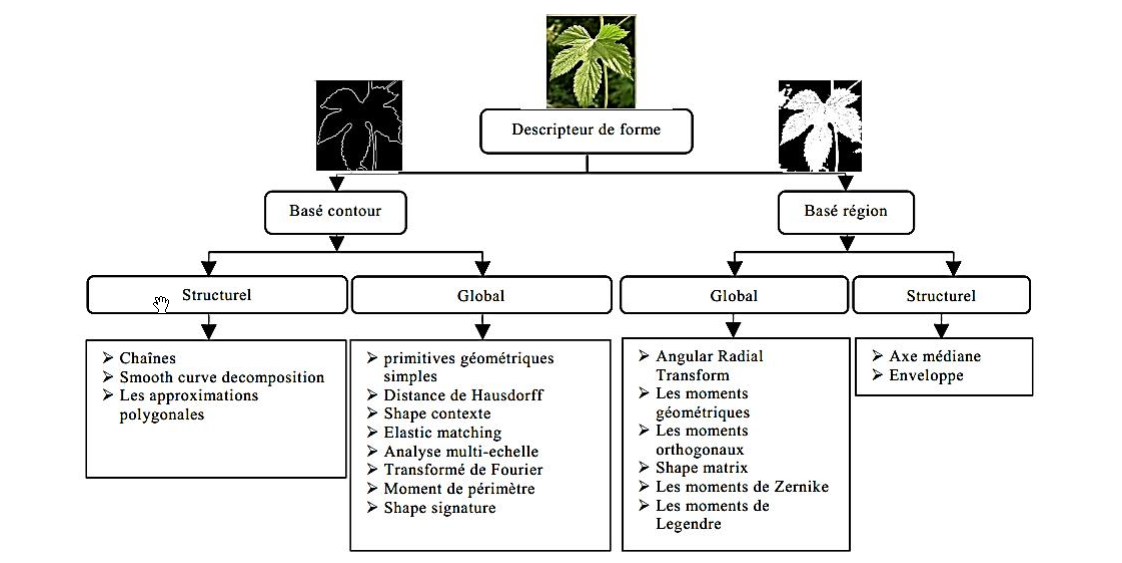
\includegraphics[width=1\textwidth]{Figures/forme} % Include the image .png
	
	\caption{Classification des méthodes d'extraction de forme.}
	
\end{figure}

Le problème fondamental est de déterminer si deux objets sont similaires, indépendamment de leur position dans l’image. C’est-à-dire l’invariance aux similitudes planes (Translation suivie d'une rotation et d’une homothétie). Il est bien connu que les descripteurs de forme invariants doivent satisfaire certains critères parmi lesquels : la robustesse vis à vis des faibles variations de formes et des approximations numériques, et la simplicité pour le calcul en « temps réel ».\\

Dans la suite nous présentons quelques-unes de ces méthodes.

\subsubsection{Descripteurs de Fourier}
Les descripteurs de Fourier (DFs) font partie des descripteurs les plus populaires pour les applications de reconnaissance de forme et de recherche d'images. Transformée de Fourier est une représentation fréquentielle d’une image, elle consiste de remplacer chaque région par des différentes fréquences spatiales. Les descripteurs de Fourier font partie des descripteurs basés sur les contours, ils ont souvent été utilisés par leur simplicité et leurs bonnes performances en terme de reconnaissance [Zhang05] et facilitent l'étape d’appariement. De plus, ils permettent de décrire la forme de l’objet à différents niveaux de détails.\\

Les DFs sont calculés à partir du contour des objets. Leur principe est de représenter le contour de l'objet par un signal 1D, puis de le décomposer en séries de Fourier. Les DFs sont généralement connus comme une famille de descripteurs car ils dépendent de la façon dont sont représentés les objets sous forme de signaux.

\subsubsection{Moments géométriques}
Les moments géométriques [Sonka99] permettent de décrire une forme à l’aide de propriétés
statistiques. Ils représentent les propriétés spatiales de la distribution des pixels dans l’image. La formule générale des moments géométriques est donnée par la relation suivante :

\begin{equation}
	M_{p,q} = \sum_{x=0}^{M-1}\sum_{y=0}^{N-1} x^p y^q f(x, y)
\end{equation}

avec $p+q$ est l'ordre du moment. Le moment d’ordre 0 $(M_{0,0})$  représente l’aire de la forme de l'objet, $f(x, y)$ : luminance du pixel $(x, y)$, c’est-à-dire noir ou blanc en binaire.

Les deux moments d'ordre $1 (M_{1,0})$ et $(M_{0,1})$, associés au moment d’ordre $0 (M_{0,0})$ permettent de calculer le centre de gravité de l'objet. Les coordonnées de ce
centre sont:

\begin{equation}
		\begin{tabular}{cc}
		$\bar{x} = \frac{M_{1,0}}{M_{0,0}}$ & $\bar{y} = \frac{M_{0,1}}{M_{0,0}}$
		\end{tabular}
\end{equation}
Il est possible de calculer à partir de ces moments l’ellipse équivalente à l’objet. Afin de calculer les axes de l’ellipse, il faut ramener les moments d’ordre 2 au centre de gravité :

\begin{equation}
\begin{tabular}{ccc}
$m_{2, 0}^g = M_{2,0} - M_{0,0} \bar{x}^2$ & $m_{1,1}^g = M_{1,1} - M_{0,0} \bar{x}\bar{y}$ 
& $m_{0,2}^g = M_{0,2} - M_{0,0} \bar{y}^2$ 
\end{tabular}
\end{equation}

Puis on détermine l’angle d’inclinaison de l’ellipse $\alpha$:
\begin{equation}
    \alpha = \frac{1}{2} \arctan(\frac{2m_{1,1}^g}{m_{2, 0}^g-m_{0,2}^g})
\end{equation}

Les moments géométriques sont très robustes et peu sensibles au bruit, préservation de l’information, facilement calculés et implémentés. Par contre, cette approche a des inconvénients comme la difficulté à corréler les moments avec la forme en elle-même, très sensible aux déformations et le temps de calcul de ces moments est très long.

\subsubsection{Les  moments de Hu}
À partir des moments géométriques, Hu [Hu62] a proposé en 1962 un ensemble de sept moments appelés moments de Hu. Ils sont invariants aux translations, rotation et changement d’échelle pour décrire une image. Par contre, ils sont très sensibles au bruit ce qui peut être un gros inconvénient dans un système de recherche d’images.\\

Nous les présenterons dans le chapitre 4.


\subsubsection{Moments orthogonaux}
Par opposition aux moments géométriques qui sont définis par rapport à une base quelconque $(x^p, y^q)$, les moments orthogonaux, comme leur nom l’indique, sont définis dans une base orthogonale, ce qui évite la redondance des informations portées par chacun des moments. Les deux types de moments orthogonaux les plus utilisés sont : les moments de Legendre et les moments de Zernike. (Les moments de Zernike a voir dans le chapitre 4) .

\subsubsection{Transformation ART}
Angular Radial Transform (ART) est un descripteur de forme robuste au changement d’échelle, à la translation et à la rotation et utilisé dans plusieurs travaux [Chawki16] et [AlAsnaoui17]. Ce descripteur consiste à projeter l’objet à étudier sur une série de fonctions de base [Kim99].

ART est un descripteur de formes par approche région qui caractérise la distribution des pixels dans un objet ou une région 2D. Il est basé sur l’étude des frontières et des pixels internes de la région à décrire. Il s’applique à un grand nombre d’objets, comme des objets complexes constitués de multiples régions discontinues ou des objets simples avec ou sans trou. Le descripteur de formes par approche régions se calcule en décomposant la forme sur plusieurs fonctions de base 2D orthogonales, définies par la transformation ART. Les coefficients ainsi obtenus sont utilisés après normalisation et quantification pour décrire la forme. ART donne un moyen compact et efficace pour exprimer la distribution de pixels dans une région de l’objet 2D [AlAsnaoui17]. Il peut décrire les deux formes de la région connectés et déconnectés.\\

L’ART [Kim99] décrit une forme à travers la distribution de ses pixels de façon invariante aux transformations affines. La transformation ART est utilisée comme descripteur par approche
région dans le standard MPEG-7. Elle est définie par la formule suivante :

\begin{equation}
    F_{nm} = {\int }_0^{2\pi} {\int }_0^{1} V_{nm}(\rho, \theta) f(\rho, \theta) \rho d\rho  d\theta
\end{equation}

Dans cette formule, $ F_{nm} $ est un coefficient d’ART d’ordre $ n $ et $ m $ , $ f(\rho, \theta) \longrightarrow {0,1} $ est une fonction image binaire définie en coordonnées polaires, et$  V_{nm}(\rho, \theta) $ st une fonction de base d’ART qui est séparable dans la direction angulaire et radiale :
\begin{equation}
	V_{nm}(\rho, \theta)= A_m(\theta) R_n(\rho) 
\end{equation}
où
\begin{equation}
\begin{tabular}{cc}
 $ A_m(\theta) =\frac{1}{2\pi}\exp(jm\theta) $ 
    & $ R_n(\rho) = \left\{
    \begin{array}{cc} 
    1 & n=0 \\ 2\cos( n \pi \rho) 
    & n \neq 0  \end{array} \right. $ 
\end{tabular}
\end{equation}

Le descripteur ART est alors défini comme l’ensemble des coefficients $ F_{nm} $ où $ m $ et $ n $ désignent les nombres de coefficients considérés.

 \begin{figure}[H]
	\label{fig:art}
	\centering
	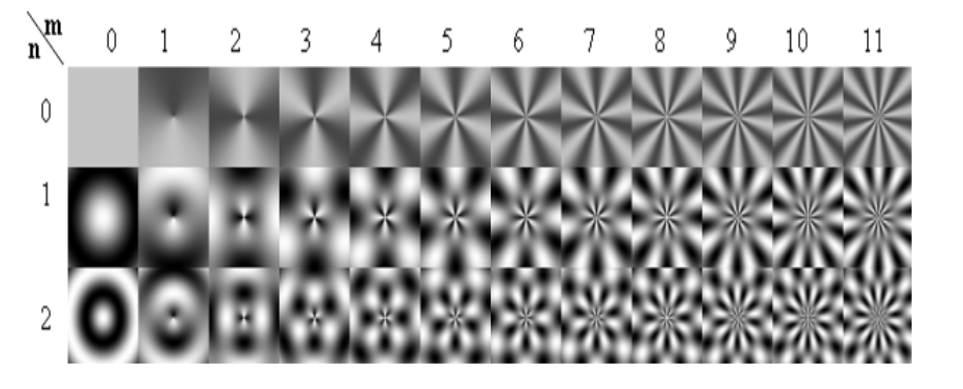
\includegraphics[width=0.65\textwidth]{Figures/art} % Include the image .png
	
	\caption{Parties réelles des fonctions de base d’ART.}
	
\end{figure}

La fonction de base d’ART $ V_{nm} $ est une fonction complexe. Sur la figure ci-dessus (Figure 2.10), les parties imaginaires sont identiques aux parties réelles, avec une différence de phase. La partie réelle de chaque fonction de base est présentée sous forme d’images.\\

Pour chaque image donnée, il y aura $ n \times m $  coefficients ART. Ces coefficients sont utilisés pour mettre en correspondance deux images. Le problème est de savoir combien de coefficient est nécessaire pour la description d’une image. Pour déterminer le nombre de coefficients, il faut analyser les covariances entre les fonctions de base. Par définition, le comité MPEG-7 [Jean01] maintient le nombre des valeurs de n plus petit que celui de m. Il propose de fixer n à 3 et m à 12. Ce sont les valeurs que nous utilisons dans notre étude.\\


Les méthodes d’indexation et de recherche doivent posséder les propriétés d’invariance aux
transformations géométriques subies par un objet à l’intérieur d’une image. ART présente certains avantages tels que :
\begin{itemize}
	\item  Robustesse aux changements d’échelle et aux translations.
	\item Invariance aux rotations.
	\item  Robustesse à la présence de bruit.
\end{itemize}

%\subsubsection{Conclusion}
%L'information relative à la forme est particulièrement importante dans la description d'une image. Plusieurs études ont été menées pour trouver un critère de choix des descripteurs de la forme pour l'indexation des images pour combler les manques des descripteurs couleur et texture.\\
%
%Pour rechercher des formes similaires, des mesures de similarité entre des descripteurs sont définies pour déterminer la distance entre eux. Cependant, la comparaison n’est pas toujours simple et elle exige parfois des transformations. De plus, la dimension du descripteur est souvent élevée, ce qui augmente la complexité quand on cherche des objets similaires dans une grande collection.\\
%
%Dans ce qui suit, nous présenterons quelques mesures de similarités utilisé en recherche d'images par contenu.

%
% Les descripteurs basés sur le contour incluent les descripteurs de Fourier [Rui 98], [Zhang 05], et les chaînes de Freeman, qui ont été largement utilisés.
% 
%  Les descripteurs basés sur la région prennent en compte tous les pixels de la forme et les méthodes les plus courantes sont basées, sur la théorie des moments [Prokop 92], [Hu 62], [Jiang 91], [Taubin 92].
%   
%   Les moments invariants offrent une description robuste aux transformations affines, propriété appréciable pour les systèmes CBIR.
%
%Quelle que soit la méthode utilisée, il demeure important que certaines propriétés d'invariance soient vérifiées, notamment pour la translation, le changement d’échelle et la rotation, du fait que l’être humain corrige instinctivement les effets de ces transformations lors de la recherche d’un objet. Dans certaines applications, la robustesse à l’occultation peut également être souhaitée.
%


\section{Les mesures de similarité entre attributs}
L'étape de la recherche dans les systèmes CBIR est la raison d'être d'un tel système et nécessite des techniques de comparaison entres attributs d'image (signatures). La mesure de similarité est alors une étape fondamentale dans la recherche d'images par le contenu. Elle compte sur la mesure de la ressemblance visuelle entre une image requête et les images de la base.\\

Les performances d'un CBIR dépendent largement de la mesure de similarité utilisée pour la comparaison des descripteurs des images.  de la recherche mais également de la représentation des caractéristiques.\\

La mesure de similarité quantifie la proximité des images dans l'espace des caractéristiques. Elle est souvent métrique, les images sont considérées ressemblantes si la distance est faible. La complexité de calcul d'une distance doit être raisonnable par ce que dans un système CBIR cette tâche s'exécute en temps réel ou pseudo réel. D'autres paramètres entrent en jeu telle la dimension de l'espace caractéristique, la taille de la base... La méthode naïve de recherche calcule la distance entre la requête et toutes les images de la base puis les ordonne selon leur score. Ceci par conséquent rend le temps de réponse proportionnel au nombre d'images $ (O(N)) $. Les méthodes d'indexation du contenu permettent par ailleurs de réduire cette complexité comparée à la recherche séquentielle (Exemple de M-Tree que nous présenterons dans le chapitre qui suit). 

Pour résumer, la mesure de similarité vérifie généralement les propriétés [Houari10]:

\begin{itemize}
	\item  \textbf{La perception} : Une faible distance dans l'espace de caractéristique indique deux images semblables.
	
	\item \textbf{Le calcul} : La mesure de distance se calcule rapidement pour une faible latence.
	
	\item \textbf{La scalabilité }: Le calcul de distance ne doit pas être affecté par une modification de taille de la base.
	
	\item \textbf{La robustesse} : La mesure devra être robuste aux changements des conditions d'acquisition d'image.
\end{itemize}

En mathématiques, on appelle distance sur un ensemble $E$ une application $d$ définie sur le produit $E^2 = E \times E$ et à valeurs dans l'ensemble $R^+$ des réels positifs:

\begin{equation}
	d: E \times E \rightarrow R^+
\end{equation}

vérifiant les propriétés suivantes :
\begin{table}[H]
	\caption{Les propriétés d'une distance.}
\begin{figure}[H]
	\centering
	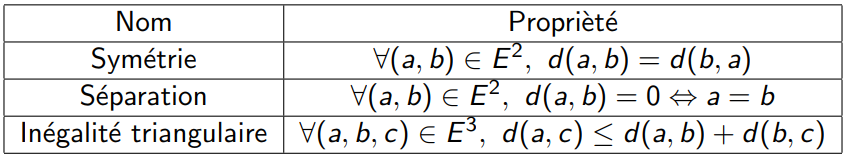
\includegraphics[width=0.8\textwidth]{Figures/distanceProp.png} % Include the image .png
\end{figure}
\end{table}

Un ensemble muni d'une distance est un espace métrique.\\

Au lieu d'un appariement exact, la recherche d’images par le contenu calcule des similarités visuelles entre une image requête et les images de la base d'images. En conséquent, le résultat d'une recherche n'est pas une seule image mais une liste d'images ordonnées selon leur degré de similitude avec l'image requête. Plusieurs mesures de similarités ont été proposées dans la littérature. Les différentes mesures de similarité influencent les performances de recherche des systèmes de recherche par le contenu.\\

Le choix de la mesure de similarité la plus appropriée dépend du niveau d'abstraction de la
représentation de l'image : images brutes (pixels) ou attributs (vecteurs descripteurs).
\begin{itemize}
	\item \textbf{Images brutes (pixels): }Au plus bas niveau d'abstraction, les images sont tout simplement des agrégations de pixels. La comparaison entre les images, est réalisée pixel par pixel, et les mesures de similarité couramment utilisées comprennent : le coefficient de corrélation, la somme des valeurs absolue des différences (SVAD), la distance des moindres carrés, et l’information mutuelle.
	La comparaison au niveau des pixels est très spécifique et, par conséquent, n'est utilisée que lorsque des appariements relativement précis sont nécessaires.
	
	\item \textbf{Attributs:} Les attributs ou vecteurs descripteurs sont des valeurs numériques de données extraites des images ou des objets dans les images, tels que la couleur, la forme et la texture. Plusieurs mesures de similarité sont couramment utilisées pour la comparaison d’attributs: la distance euclidienne, la distance de Minkowsky et la distance d’intersection  [Khouloud09].
\end{itemize}

Julien Fauqueur à classifier les distances pour les distributions de couleurs [Fauqueurs03] comme suite:
\begin{table}[H]
	\centering
	\caption{Les classe de distances.}
	\begin{tabular}{|l|l|l|}
		\hline
		\textbf{\makecell{Distances cellule-à-cellule ou “daltoniennes”}
} & \textbf{Distances inter-cellules}\\
		\hline
		\makecell{- Les distances de Minkowski\\
		- Intersection d’histogrammes\\
	    - Test du $ \chi^2 $  \\
        - Divergence de Kullback Leibler\\
        - “Jensen Difference Divergence”} 
		& \makecell{- Histogramme cumulé\\
			- Histogramme flou \\ 
			- Distance Quadratique\\
			- Earth Mover Distance\\
			- “Weighted Correlation”
		 }   \\
		\hline 
	\end{tabular}
	
\end{table}

Ci-après les distances les plus utilisées pour comparer des images considérées comme vecteurs ou comme distributions statistiques. 

\subsection{Distances de Minkowski}
La distance de Minkowski est une famille de distances vectorielles. Soit $I_1$ , $I_2$ deux vecteurs de caractéristiques, elle s'exprime par :

\begin{equation}
        d_p(I_1, I_2) =  \sqrt[p]{\sum_{i=1}^{N} \left|{I}_{1}(i)-{I}_{2}(i)\right|^p} 
\end{equation}

Où $p\geq 1$ est le facteur de Minkowski et $N$ la dimension de l’espace caractéristique. Les métriques de Minkowski sont simples d’utilisation, rapides à calculer, simples à implémenter, et représentent un bon compromis entre efficacité et performance, par contre leur calcul est réalisé en considérant que chaque composante du vecteur apporte la même contribution à la distance. Pour cette famille de distances, plus le paramètre $p$ augmente, plus la distance $d_p$ aura tendance à favoriser les grandes différences entre coordonnées.

On distingue:
\begin{table}[H]
	\caption{Les distances de Minkowski}
	\begin{tabular}{|c|c|c|}
		\hline
		\textbf{Distance} & \textbf{Caractéristiques}\\
		\hline
		\makecell{Manhatttan : \\ $  d_1(I_1, I_2) = \sum_{i=1}^{N} \left|{I}_{1}(i)-{I}_{2}(i)\right|  $ } 
		& \makecell{Cette distance est plus convenable pour mesurer\\
			  la similarité entre les données  multivariées,\\ 
			 elle est moins sensible au  bruit\\
			 coloré que la distance euclidienne. }   \\
		\hline
		
		
		\makecell{Euclidienne :\\ $ d_2(I_1, I_2) =  \sqrt{\sum_{i=1}^{N} \left|{I}_{1}(i)-{I}_{2}(i)\right|^2} $}  
		& \makecell{C’est la distance la plus fréquemment \\
			utilisée grâce à ses propriétés géométriques \\
			intéressantes. Cette distance à tendance à \\
			donner plus d’importance aux plus grandes \\
			différences sur une variable simple. Le contour\\
			 de la même distance (Euclidienne) à partir d’un \\
			 point donnée à  une forme sphérique \\(cercle en deux dimensions).}   \\
		\hline
		
		\makecell{Chebychev :\\ 
			$d_{\infty}(I_1, I_2)=\max_{i=1}^N \left|{I}_{1}(i)-{I}_{2}(i)\right|$  
		} 
		 & \makecell{La distance de Chebychev est adaptée \\
		 	aux données de grande dimension, elle est \\
		 	souvent employée dans les applications où la\\
		 	 vitesse d’exécution est importante.\\ 
		 	 Cette distance examine la différence absolue\\
		 	  entre les différents pairs des vecteurs, elle\\
		 	   est considérée comme une approximation\\ 
		 	   de la distance Euclidienne mais\\
		 	    avec moins de calcul.} \\   
		\hline
		
	
	\end{tabular}
	
\end{table}

\subsection{Distance quadratique}
La distance de Minkowski traite les éléments du vecteur de caractéristique d’une manière équitable. La distance quadratique en revanche favorise les éléments les plus ressemblants. Les propriétés de cette distance la rendraient proche de la perception humaine de la couleur, ce qui en fait une métrique attractive pour les systèmes de Recherche d’images couleur par le contenu. Proposée dans [Hafner95], la distance couleur quadratique compare toutes les valeurs
de cellules des deux histogrammes qu’elle pondère par leur similarité couleur, Sa formule générale est donnée par :

	\begin{equation}
	d_q(I_1, I_2) = \sqrt{(I_1 - I_2)^T A (I_1 - I_2)} 
	\end{equation}



Ou $A = (a_{ij}) $est la matrice de similarité. $a_{ij}$ représente la distance entre deux éléments des vecteurs $I_1$ et $I_2$, elle est définie par :


\begin{equation}
	a_{ij} = 1 - \frac{d_{ij}}{ d_{max}} 
\end{equation}

Où $ d_{ij} $ est la distance dans l’espace couleur considéré et $ d_{max} $ le maximum global
de cette distance. Notons que si l’on remplace $  A $ par la matrice identité, nous retrouvons la distance euclidienne.
\subsection{Distance de Swain}
Cette mesure est l'une des premières distances utilisée dans la recherche d'image par le contenu, si les images d’une base des images sont indexées par des histogrammes, les distances géométriques s’appliquent. Cependant, il est possible de définir des mesures de similarité propres à cette représentation. Ainsi, l’intersection d’histogrammes est l’une des premières distances utilisée dans les systèmes CBIR [Swain91]. Elle permet de comparer deux histogrammes normalisés $H_1$ et $H_2$ . La distance de Swain s’exprime ainsi :

	\begin{equation}
	 d_2(H_1, H_2) = 1- \frac{\sum_{i=1}^{N} \min(H_1(i),  H_2(i))}{\sum_{i=1}^{N}  H_2(i)}  
	\end{equation}

\subsection{Distance de Canberra}
Elle est introduite par G. N. Lance et W. T. Williams [Lance67]. C'est une version
pondérée de la distance Manhattan. La distance de Canberra entre les vecteurs et dans un espace vectoriel réel à N dimensions est la suivante:

\begin{equation}
	d_c(I_1, I_2) = 1- \sum_{i=1}^{N}   \frac{\left|{I}_{1}(i)-{I}_{2}(i)\right|}{\left|{I}_{1}(i)\right| + \left|{I}_{2}(i)\right|}
\end{equation}


Il existe d’autres distances dans la littérature qui ne sont pas abordées dans ce mémoire.


\subsection{Conclusion}
Le choix des descripteurs ou mesures de similarité pour un système de recherche d'images par contenu est important, dans le sens où, ce choix influe sur les résultats attendus. Cependant, d'une part il n'y a pas d'attributs universels, et d'autre part le choix des descripteurs dépend fortement de la base d'image à utiliser et des connaissances à priori qu'on peut avoir sur la base.\\

Ce chapitre a fait l’état de l’art sans exhaustivité des différents descripteurs des attributs visuels pouvant être utilisés pour la recherche d’images par le contenu ainsi que les approches correspondantes. Aussi, nous avons dressé une liste des types de descripteurs et les mesures de similarités avec leurs avantages et leurs inconvénients. Le chapitre suivant se focalisera sur les méthodes d'indexation pour accélérer la recherche et leurs importance dans un systeme CBIR. 
% Chapter Template

\chapter{Apport de la structure d’index M-Tree dans un CBIR} % Main chapter title

\label{Chapter3} % Change X to a consecutive number; for referencing this chapter elsewhere, use \ref{ChapterX}

%----------------------------------------------------------------------------------------
%	SECTION 1
%----------------------------------------------------------------------------------------

\section{Introduction}
Dans les systèmes de recherche d'images par le contenu le temps d'exécution d'une requête est d'une importance primordiale. Pour répondre aux besoins d'un CBIR d'être robuste en temps du calcul lors de l'étape d'indexation et l'étapes de recherche de nombreuse méthodes d'indexation ont vu le jour. Parmi ces méthode ou structures on trouve la structure M-tree, une structure recherche par similarité dans les espaces métriques, que nous avons choisi pour la partie d'accélération de recherche dans notre sujet. \\
 
La discussion du sujet de recherche par similarité dans les espaces métriques soulève plusieurs questions. Tout d’abord, les premières questions qui se posent sont des questions sur les espaces métriques comme : quelles sont les propriétés et les caractéristiques des espaces
métriques ? Ensuite, quelles sont les fonctions de similarité qui répondent aux critères des distances métriques? Quels sont les types des requêtes souvent utilisées pour chercher dans les espaces métriques?\\

Enfin, la discussion de recherche par similarité dans les espaces métriques conduit forcément à poser des questions sur les méthodes métriques d’indexation et de recherche, quelles sont les méthodes principales de recherche par similarité dans les espaces métriques
qui sont proposées dans la littérature, et quels sont les avantages et les inconvénients de chaque méthode?

Ce chapitre vise à discuter ce sujet afin de surligner les déférents concepts y liés.
\section{L’espace métrique}
Etant donné un ensemble E des objets, chaque fonction $d: E\times E\rightarrow R^+$ qui satisfait les trois propriétés suivantes est appelée une distance:

\begin{equation}
	\begin{array}{cc}
	(p1) \textbf{La positivité} : & \forall (x,y)\in E^2, d(x,y) \ge 0 \\
	(p2) \textbf{La symétrie} : & \forall (x,y)\in E^2, d(x,y) = d(y,x) \\
	(p3) \textbf{Réflexivité} : & \forall (x,y)\in E^2, d(x,y) = 0 \Rightarrow x = y
	\end{array}
\end{equation}

Une distance métrique est une distance qui satisfait les trois propriétés ci-dessus plus une quatrième propriété. Cette propriété est connue sous le nom « l’inégalité triangulaire », elle est définie formellement comme le suivant :

\begin{equation}
\begin{array}{cc}
(p4)\textbf{ L’inégalité triangulaire :}  & \forall x,y,z\in E, d(x,y)+d(y,z) \geq d(x,z)
\end{array}
\end{equation}

\begin{description}
	\item[Définition 1:] Un espace Métrique $ (E,d) $ est un ensemble $ E $ muni d’une distance métrique $ d $.
\end{description}

Dans le paradigme de recherche par similarité, la distance entre les objets représente le degré de ressemblance entre ses objets, c.à.d si la distance entre deux objets est petite, cela signifie que ces deux objets sont fortement similaires, et par contre, si la distance est assez grande, les objets sont assez dissimilaires.

\subsection{Les requêtes de recherche par similarité dans les espaces métriques}
La recherche d’informations dans une base de données peut se faire par plusieurs manières. Dans la suite de cette partie nous présentons deux types intéressants de requêtes largement utilisées dans la recherche par similarité dans les espaces métriques, il s’agit de la requête intervalle et la requête des k plus proches voisins.

\subsubsection{La requête intervalle (Range Query R(q,r))}
Ce type consiste à sélectionner dans la base tous les objets dont la distance par rapport à l’objet de la requête $ q $ est inférieure au rayon de recherche $ r $. Formellement, on peut définir la requête intervalle de la manière suivante.\\

\textbf{Définition 2:} Soit $ (E,d ) $ un espace métrique, $ q $ un objet requête et $ r $ est un réel  positif. La requête par intervalle $ R(q,r) $ retourne l’ensemble défini par :
\begin{equation}
	R = \left\{ o\in E / d(o, q) \leq r \right\}
\end{equation}

\begin{figure}[H]
	\centering
	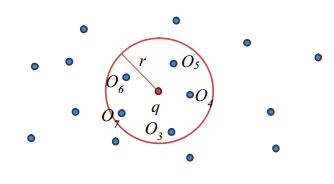
\includegraphics[width=0.65\textwidth]{Figures/rangeQ} % Include the image .png
	\caption{Exemple de la requête intervalle.}
\end{figure}
La Figure 3.1 représente un exemple d’une requête par intervalle dans un espace de
deux dimensions, l’exécution de la requête $ R(q,r) $ retourne le sous-ensemble qui contient les objets $ {O_3,O_4,O_5,O_6,O_7} $.

\subsubsection{La requête des k plus proches voisins kpp (k-NN R(q,k))}
Cette requête consiste à retourner les $ k $ objets les plus similaires à l’objet de la requête $ q $. Formellement, la recherche des $ k $ plus proches voisins est définie comme suite :

\textbf{Définition 3:} Soit $ (E,d ) $ un espace métrique, $ q $ un objet requête, et $ k \in \mathbb{N} $. Alors, la requête  $ R(q,k) $ des $ k $ plus proches voisins $ k $-ppv retourne un sous-ensemble R des objets telle que

\begin{equation}
R = \left\{ o_1,...,o_k \in E / \forall o \in E, d(o, q) \ge \max_{1\leq i \leq k}\left\{d(o_i, q)\right\}  \right\}
\end{equation}

\begin{figure}[H]
	\centering
	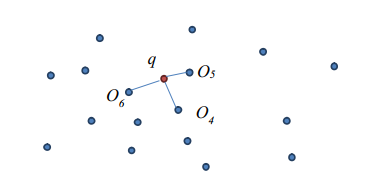
\includegraphics[width=0.65\textwidth]{Figures/knnQ} % Include the image .png
	\caption{Exemple de la requête des k plus proches voisins.}
\end{figure}
La Figure 3.2 représente un exemple d’une requête des k plus proches voisins, l’exécution d’une requête de trois plus proches voisins de la requête q retourne les trois objets $ O_4 $, $ O_5 $ et $ O_6 $.

Nous avons effectuer une expérience pour comparer entre la performance de recherche linéaire et de recherche des k-NN de M-Tree. Nous avons effectuer la recherche dans une liste triée allant de 0 à 2001 avec des valeurs différentes à chaque test; n = 10, 100, 200, ..., 2000. la recherche linéaire retourne une seul valeur contre k=6 valeurs retourné par k-NN. Par ce fait, nous observons l'intérêts des structures d'index dans la figure 3.3 qui montre que M-tree accélère la recherche.
\begin{figure}[H]
	\centering
	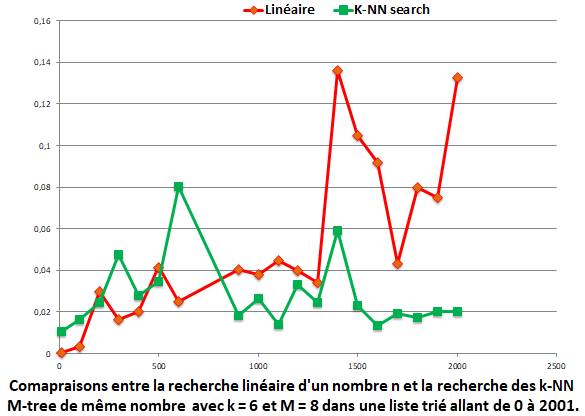
\includegraphics[width=0.65\textwidth]{Figures/mtreeVSlinear.png} % Include the image .png
	\caption{Comapraisons entre la recherche linéaire et la recherche des k-NN M-tree.
	}
\end{figure}


\subsection{Les fonctions métriques}
Les fonctions métriques sont des fonctions qui permettent de mesurer la distance entre les objets d’un espace métrique. Le choix de la distance métrique convenable de comparaison se fait selon le type des données traitées, en effet, chaque type d’espace métrique à des distances métriques appropriées qui sont spécifiées par les experts. Généralement, les distances métriques sont classifiées en deux catégories [Chávez01]: les distances discrètes et les distances continues. Le choix de distance influence directement sur l’efficacité de la structure utilisée, et le choix de type de distance adéquate, pour construire une telle structure, dépend fortement de la base traitée [Hanif18]. Dans ce qui suit, un aperçu général sur quelques exemples de fonctions métriques continues et des fonctions métriques discrètes.

\subsubsection{Distances Continues}
Les distances continues sont des fonctions métriques qui peuvent retourner un ensemble infini des valeurs. Généralement, elles sont calculées en se basant sur les coefficients des objets. Dans ce qui suit  on donne l'exemples le plus connue des distances continues, La famille des distances de Minkowski Lp est un ensemble des distances continues, elles sont définies formellement par:
\begin{equation}
L_p(I_1, I_2) = \sqrt[p]{\sum_{i=1}^{N}  \left|{I}_{1}(i)-{I}_{2}(i)\right|^p} 
\end{equation}

\begin{itemize}
	\item Manhatttan :  $  L_1(I_1, I_2) = \sum_{i=1}^{N} \left|{I}_{1}(i)-{I}_{2}(i)\right|  $ 
	
	\item Euclidienne : $ L_2(I_1, I_2) =  \sqrt{\sum_{i=1}^{N} \left|{I}_{1}(i)-{I}_{2}(i)\right|^2} $
	
	\item Chebychev : 
	$L_{\infty}(I_1, I_2)=\max_{i=1}^N \left|{I}_{1}(i)-{I}_{2}(i)\right|$  
\end{itemize}

\begin{figure}[H]
	\centering
	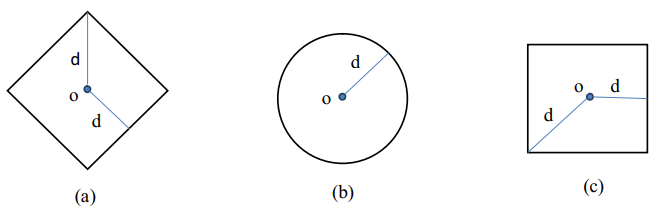
\includegraphics[width=0.5\textwidth]{Figures/mink} % Include the image .png
	\caption{Exemples des distances de la famille Lp:\\ (a) $ L_1 $ (b) $ L_2 $ (c) 	$L_{\infty}$}
\end{figure}

\subsubsection{Distances Discrètes}
Les distances discrètes sont des distances métriques qui ne retournent qu’un nombre limité des valeurs. Généralement, elles sont calculées en se basant sur la comparaison des coefficients des objets pour retourner le nombre des objets qui sont identiques ou le nombre des coefficients qui se diffèrent. Dans la suite de cette section, on présente deux exemples des distances discrètes.

\paragraph{La distance Edit:}
La fonction edit [Levenstein65] est une métrique pour mesurer la distance entre les chaines de caractère. Elle représente le nombre minimal des opérations suffisantes pour convertir une chaine en une autre. Par exemple, on considère deux chaines de caractère $x=x_1x_2...x_n$ et $y=y_1y_2...y_m$, la distance $edit(x,y)$ entre l’objet $x$ et $y$ c’est le nombre des opérations pour convertir la chaine $x$ à $y$. Les opérations qui peuvent être utilisées sur une chaine de caractère sont définies comme suit :
\begin{itemize}
	\item Insérer : pour insérer un caractère dans une position donnée de la chaine
	\item Supprimer : pour supprimer un caractère de la chaine
	\item Remplacer : pour remplacer un caractère d’une position donnée dans la chaine par un autre caractère
\end{itemize}
Edit distance est une distance discrète souvent utilisée pour mesurer la similarité des documents texte et pour manipuler des données scientifiques comme les ADN et les protéines.

\paragraph{La distance de Hamming:}
La distance de Hamming est une distance discrète proposée en 1950 [Hamming50], elle sert à calculer la distance entre les vecteurs. La distance Hamming entre les vecteurs A et B représente le nombre des coefficients qui se diffèrent, si la distance est égale à 0, ça signifie que les vecteurs A et B sont identiques. Formellement, on peut définir la distance de Hamming comme suite:

\begin{equation}
d_h((x_1,...,x_n), (y_1,...,y_n)) = card(\left\{ i: x_i \neq y_i, 1\leq i \leq n\right\})
\end{equation}
Par exemple, la distance de Hamming entre les deux vecteurs $ (1,2,1,3) $ et $ (0,2,3,1) $, et la distance de Hamming entre les deux chaines de caractères « BFEC » et « BFAC » sont calculées comme suit :

\begin{tabular}{cc}
	 $ d_h ((1,2,1,3), (0,2,3,1))= Card({1,3,4}) = 3 $ &  $d_h(BFEC , BFAC)= Card({3}) = 1 $ \\
	 \\
\end{tabular}

L’utilisation de la distance de Hamming est très large [Deza09], elle peut être utilisée pour mesurer de similarité de déférent type des donnés comme images, DNA, Protéine et Textes.

\section{Les données métriques}
La plupart des données acquises aujourd’hui peuvent être modélisées  des objets dans un espace métrique muni d’une distance métrique. Dans cette section, nous présentons des exemples des types bases de données qui peuvent utiliser des distances métriques pour faire la recherche par similarité.

\subsection{Les images 2D}
L’extraction automatique des caractéristiques d'images directement à partir de leur contenu numérique est une solution parmi les solutions possibles pour gérer efficacement les bases de données d'images. Chaque image est représentée par un ou plusieurs vecteurs qui représentent leurs contenus visuels. Par conséquence, la similarité entre deux images peut être mesurée par la comparaison entre leurs descripteurs. La génération d’une base de descripteurs des images représente une phase nécessaire dans les systèmes de recherche d’image par contenu. La description de contenu d’image est souvent faite par des descripteurs de bas niveau, appelés aussi vecteurs caractéristiques, tels que la couleur, la texture et la forme.

\begin{figure}[H]
	\centering
	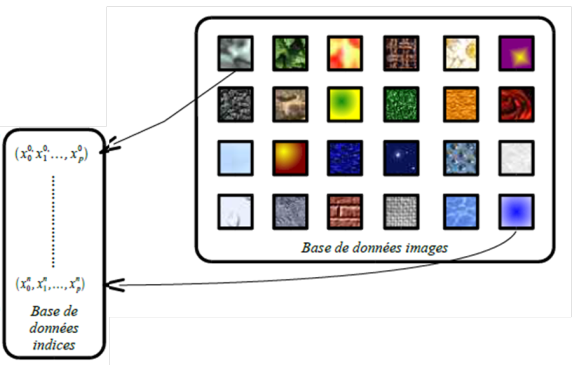
\includegraphics[width=0.55\textwidth]{Figures/horsligne.png} % Include the image .png
	\caption{Exemple de la représentation vectorielle d'une base d'image et d'une image requête.}
\end{figure}
La Figure 3.5 représente un exemple de l’extraction du contenu visuel des images sous forme des vecteurs ; A partir d’une base d’image on peut obtenir une base des vecteurs caractéristiques (indexes) qu’on peut comparer par des distances métriques.

Les distances de Monkowski sont beaucoup utilisées pour mesurer la similarité entre les descripteurs, notamment la distance Euclidienne. 

%\subsection{Séquences d’ADN}
%L'ADN contient les instructions pour toutes les fonctions d’une cellule d’un organisme, deux séquences d’ADN similaires de deux cellules signifient que les deux cellules ont des fonctions similaires. La compréhension de la relation entre une requête d’ADN avec des séquences génomiques, déjà traitées, analysées et stockées dans une base de données, sert à aider les biologistes de bien estimer les fonctionnements de la séquence requête avant de la traiter. La structure d’ADN consiste d’une chaine linéaire des quatre nucléotides qui sont souvent représentés par quatre Alphabets A, C, G et T. La Figure II-6 montre un exemple d’une
%représentation d’un gène humain [WilliamsZobel02].
%
%\begin{figure}[H]
%	\centering
%	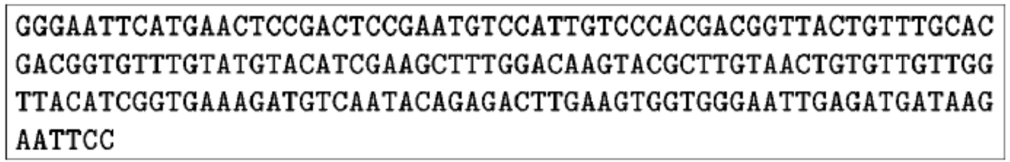
\includegraphics[width=0.55\textwidth]{Figures/ADN} % Include the image .png
%	\caption{Une partie de gène de croissance épidermique humain.}
%\end{figure}
%
%Les séquences génomiques peuvent se modéliser comme un espace métrique muni d’une distance métrique comme la distance Edit et la distance de Hamming.

\section{Les méthodes d’accès Métriques}
L'objectif principal des méthodes d’accès métrique (MAM) est la minimisation du temps de recherche. Le calcul de distance entre les objets métriques est souvent coûteux et consomme beaucoup du temps. Par exemple, le calcul des distances de Minkowski consomme un temps de complexité linéaire, le calcul de la distance Edit entre deux chaines de taille m et n est d’ordre $ O(n\times m) $. De même, la complexité de la distance de Hamming est d’ordre $ O(n\times m) $,certaines distances usuelles peuvent atteindre une complexité d’ordre $ O(n^4)  $ comme la distance Edit-tree [Zezula06]. Donc, la complexité de comparaison d’objets dans une base est un critère crucial qui influence directement sur la performance de la structure métrique utilisée. La mesure de performance se calcule en fonction du nombre de distances calculées lors du parcours de structure pour répondre à une requête parce que la complexité des autres parties des algorithmes de recherche est négligeable devant la complexité de calcul de distance [Chávez01].\\

Le but de MAMs vise à minimiser le nombre de distances calculées lors du stockage et lors de la recherche par l’exploitation des distances pré-calculées et en évitant le parcours des régions inutiles sans faire des calculs supplémentaires. La Figure 3.6 illustre un exemple de cette approche dans les bases de données d’images [Chávez01].\\


La technique la plus simple pour éviter le calcul des distances est l’exploitation directe de l’inégalité triangulaire. Supposons que, les distances entre objet pivot $ p $ des objets $ o_i $ sont pré-calculées, la distance entre une requête $ q $ et les objets $ o_i $ peut être estimée sans besoin du calcul direct des distances, il suffit de calculer la distance $ d(q,p) $ entre la requête et le pivot, ensuite, toutes les distances $ d(q,o_i) $ sont majorées par $ d(q,p)+d(p,o_i) $, et avec un simple effort de calcul nous pouvons déduire que la distance $ d(q,o_i) $ est minorée par $ |d(q,p)-d(p,o_i)| $. En effet, si $ q $ présente un objet requête, $ p $ un objet pivot et $ o $ un objet de la base. Si la distance $ d(q,p) $ entre la requête et le pivot est déjà calculée et la distance entre l’objet $ o $ et le pivot est pré-calculée. On peut estimer la distance entre la requête et l’objet par la formule suivante 
\begin{equation}
    d(q,p)+d(p,o) \geq d(q,o) \geq |d(q,p)-d(p,o)|
\end{equation}

\begin{figure}[H]
	\centering
	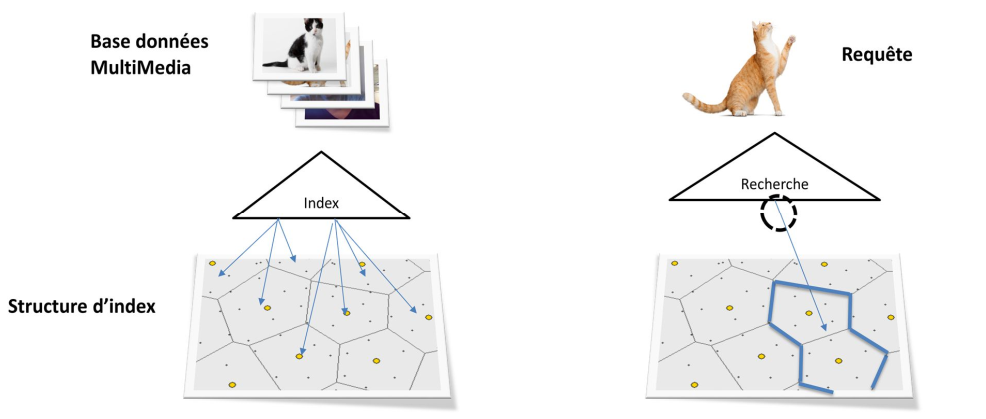
\includegraphics[width=0.6\textwidth]{Figures/similarity.png} % Include the image .png
	\caption{Modèle d'indexation métrique et la recherche par similarité.}
\end{figure}

Lors de la recherche par une requête intervalle $ R(q,r) $, les bornes supérieures et inférieures peuvent être utilisées pour accélérer la recherche. Trois situations sont possibles : si la borne supérieure est inférieure à $  r (d(q,p)+d(p,o) \leq r ) $ alors il est sûr que l’objet $ o $ est pertinent car il vérifie $ d(q,o) \leq r $, si la borne inferieure dépasse le rayon $ r ( |d(q,p)-d(p,o)| > r )  $ alors il est sûr que $ d(q,o) > r $ et par conséquence l’objet $ o $ ne peut être parmi les résultats de la requête. La dernière situation est le pire des cas, il correspond au cas où la borne supérieure est supérieure à $ r $ et la borne inférieure est inférieure à  $ r $  $  (d(q,p)+d(p,o) \geq d(q,o)\geq |d(q,p)-d(p,o)|) $, il est indispensable de calculer la distance $ d(q,o) $ pour déterminer si l’objet $ o_i $ est pertinent ou non.

\begin{figure}[H]
	\centering
	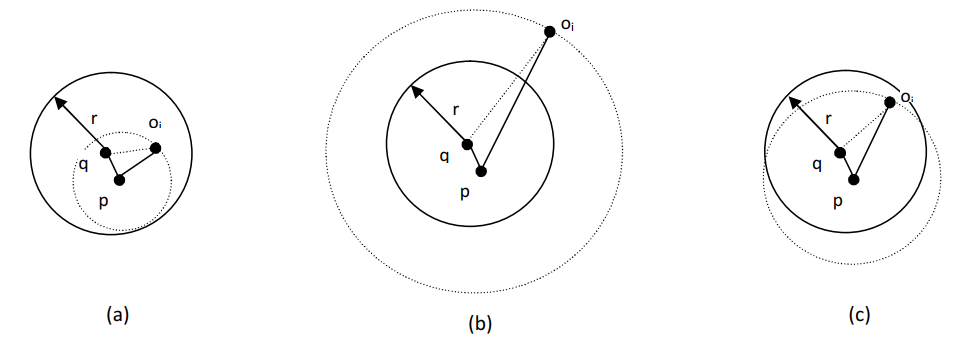
\includegraphics[width=0.6\textwidth]{Figures/pivot.png} % Include the image .png
	\caption{Filtrage par un pivot: (a) l'objet $  o_i $ fait partie du résultat (b) l'objet $ o_i $ sera éliminé (c) le calcul de la
		distance $ d(q,o_i) $ est obligatoire pour savoir si $ o_i $ est pertinent ou pas.}
\end{figure}

Les lignes solides représentent les distances connues, tandis que les lignes coupées représentent les distances non connues.\\

Pour une structure métrique qui utilise un groupe de pivots $ (p_1,p_2,…, p_n) $, les distances entre les objets $ o_i $ et les pivots sont calculées et stockées au préalable. Ainsi, lors d’une recherche par requête intervalle $ R(q,r) $, chaque objet de la base qui satisfait la condition $ \max_{i=1,..,n}{|d(q,pi)-d(o,pi)|} > r $ est certainement non pertinent et donc il sera écarté de la recherche sans aucun calcul de distance. Comme nous avons vu précédemment, le filtrage par n pivots est vu comme un « mapping » de l’espace métrique $ (E,d) $ vers un espace vectoriel $ (R^n, L_\infty) $ en lequel chaque élément $ o \in E $ est représenté par le vecteur $ (d(o,p_1), d(o,p_2),..., d(o,p_n)) $, tout objet $ o $ qui satisfait la condition $ L_\infty((d(o,p_1),..., d(o,p_n)),(d(q,p_1),..., d(q,p_n))) > r  $ sera ignoré durant la résolution d’une requête de rayon $ r $.

\begin{figure}[H]
	\centering
	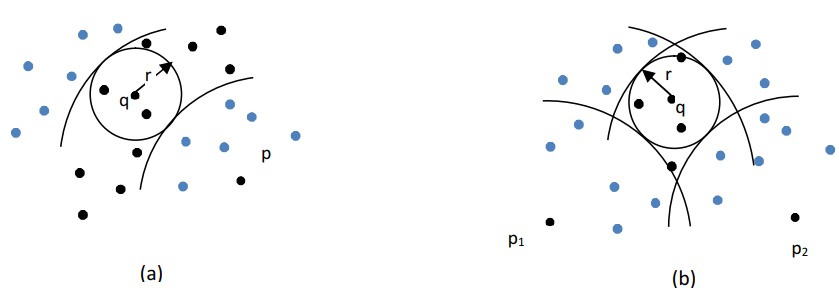
\includegraphics[width=0.6\textwidth]{Figures/npivot.png} % Include the image .png
	\caption{(a) exemple de filtrage par un pivot et (b) par deux pivots.}
\end{figure}

L’utilisation directe des pivots nécessite le stockage des distances entres les pivots et les objets dans la mémoire. Par conséquence, cette technique est coûteuse en termes de la mémoire de stockage. Pour cette raison, d'autres techniques ont été développées pour traiter ce problème comme la technique d’utilisation de double pivot et la technique de regroupement des objets dans des Clusters [Hanif18].


\begin{figure}[H]
	\centering
	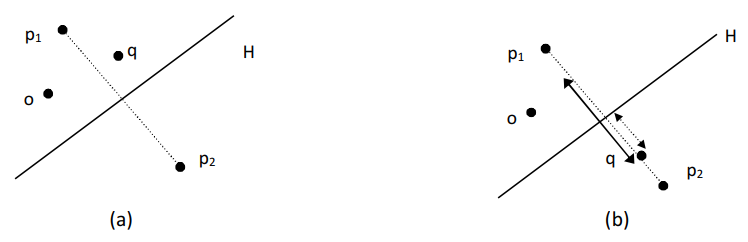
\includegraphics[width=0.6\textwidth]{Figures/2pivot.png} % Include the image .png
	\caption{L'utilisation de deux pivots pour partitionner les données, (a) représente le cas où l'objet et la requête sont dans la même partions, (b) représente le cas où l’objet est la requête situées dans des partitions différent.}
\end{figure}

La première technique est l’utilisation du double pivot qui sert à regrouper, en chaque niveau de la structure, les objets d’une manière récursive à partir de deux pivots $ p_1 $ et $ p_2 $. Les objets qui sont plus proche au pivot $ p_1 $ que le pivot $ p_2 $ seront regroupés dans la région $ S(p_1) $ du pivot $ p_1 $ et les autres objets seront regroupés ainsi dans la deuxième région $ S(p_2 $) du pivot $ p_1 $.\\

La deuxième technique sert à réduire le calcul des distances lors de stockage par l’utilisation des rayons de couverture d’un pivot au lieu de stocker les distances entre le pivot $ p $ et les objets d'une région, seulement deux valeurs $ r_{max} $ et $ r_{min} $, qui vérifie $  r_{min}  \le d(p,o) \le r_{max}  $, sont mémorisées (voir la Figure 3.10 qui suit comme un exemple). En remplaçant la distance $ d(p,o) $ par ses bornes et en utilisant la formule $ |d(q,p)-d(p,o)| \le d(q,o) \le d(q,p)+d(p,o) $, on peut facilement montrer que la distance $ d(q,o) $ est majorée par la valeur $ d(q,p) + r_{max} $ et qu’il est minorée par la valeur
$ \max \left\{d(q,p) - r_{max}, r_{min} - d(q,p), 0\right\} $,
avec:
\begin{center}
	$  ( \max \left\{ d(q,p) - r_{max} , r_{min} - d(q,p), 0\right\} \le d(q,o) \le d(q,p) + r_{max} ) $.
\end{center}
 Donc il est possible d’éviter le parcours des Clusters inutile lors de la recherche en se basant sur le pivot et les rayons de couvertures sans besoin de calcul de la distance $ d(q,o) $.
\begin{figure}[H]
	\centering
	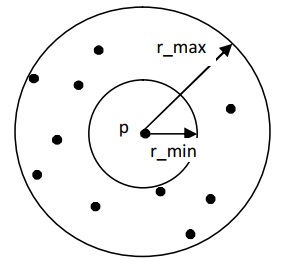
\includegraphics[width=0.25\textwidth]{Figures/radius.png} % Include the image .png
	\caption{Utilisation un pivot est de rayons de couvertures.}
\end{figure}

Dans la littérature, l’indexation de base de données par les méthodes d’accès métrique est conçue pour bénéficier d’une ou de plusieurs techniques discutées ci-dessus. On distinct entre deux approches : l’approche basée sur le partitionnement et l’approche basée sur les pivots (matrice des distances). Les méthodes basées sur les pivots construisent une matrice de distances entre les objets d’une région et les pivots afin de les utiliser pour filtrer les objets non pertinents lors de la recherche, tandis que, celle basées sur le partitionnement regroupent des objets similaires dans des régions, ce qui permet, lors de la recherche, d’éviter l’accès à des régions inutiles sans faire de calculs supplémentaires. Les taxonomie classiques souvent classifient les méthodes basées sur le partitionnent en deux catégories; le partitionnement par hyperplan et le partitionnement par boule [Chávez01]. Mais, plusieurs méthodes récentes ont dépassé cette classification soit par la proposition d’autres types de partitionnement ou par la combinaison de plusieurs types de partitionnement. \\

Plusieurs Méthodes d’accès métrique proposées en littérature sont basées sur l’idée de partitionnement des données. Elles peuvent se classifier sous quatre catégories; Les méthodes de partitionnement par boule, Les méthodes de partitionnement par hyperplan, Les méthodes de partitionnement par « Cut région » et les méthodes qui combinent plusieurs types de partitionnement [Hanif18].
\begin{figure}[H]
	\centering
	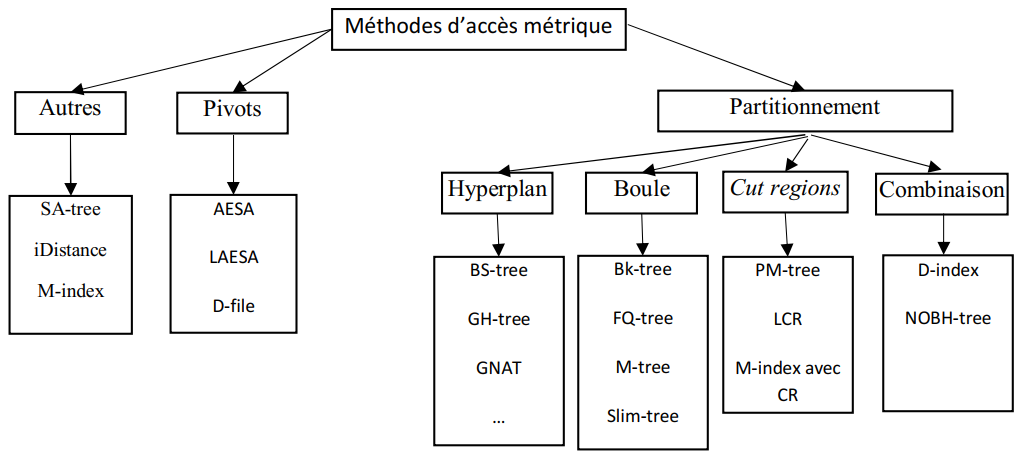
\includegraphics[width=0.55\textwidth]{Figures/class.png} % Include the image .png
	\caption{ Classification des méthodes d’accès métriques.}
\end{figure}
On s'intéresse principalement aux méthodes de partitionnement par boule.
Pour plus d'information sur les méthodes d'indexation, leurs avantages et inconvénients, le lecteur peut se référer à [Hanif18].
\section{La méthode partitionnement par boule M-tree}
Les méthodes de partitionnement en boule servent à partitionner l'espace des données sous formes des boules, elles utilisent des pivots et des rayons de couverture pour diviser les données. Le nombre des pivots utilisés, le choix du type de couverture des pivots font la différence entre les méthodes de partitionnement par boule, dans cette section nous présentons la méthodes de partitionnement par boules M-tree.

\subsection{La structuration de M-tree}
La méthode M-tree [CiPaZe97] est une structure efficace dans les environnements dynamiques caractérisés par un fréquent besoin de supprimer et d'ajouter des éléments. Le processus de construction de l'arbre M-tree consiste à partitionner l'espace métrique par des sphères région en se basant sur un pivot et un rayon de couverture. \\

M-Tree organise les objets en nœuds de taille fixe, qui correspondent aux régions de l'espace métrique. Les nœuds de l'arbre peuvent stocker jusqu'à \textbf{$ M $} entrées, c'est la capacité des nœuds. Les feuilles de l’arbre différent dans leur structure avec les nœuds internes:
\begin{itemize}
	\item Pour chaque objet indexé, une entrée au format 
	\begin{figure}[H]
		\centering
		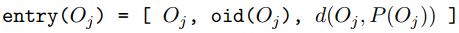
\includegraphics[width=0.6\textwidth]{entryleaf.png} % Include the image .png
	\end{figure} 
	est stockée dans un nœud feuille. Avec:
	\begin{itemize}
		\item \textbf{$ oid(O_j) $} est l'identifiant de l'objet qui réside dans un fichier de données séparé,
		\item \textbf{$ O_j $} sont les valeurs des caractéristiques de l'objet 
		\item et \textbf{$ d(O_j, P(O_j)) $} est la distance entre entre l’objet \textbf{$ O_j $} et l’objet  \textbf{$ P(O_j) $}, parent d'\textbf{$ O_j $}
	\end{itemize}

	\item Pour les nœuds internes, l'entrée stocké est au format
	\begin{figure}[H]
		\centering
		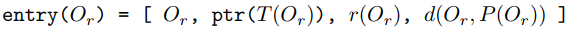
\includegraphics[width=0.7\textwidth]{entryInternal.png} % Include the image .png
	\end{figure} 
	Avec,
	\begin{itemize}
		\item \textbf{$ O_r $} est une valeur de caractéristique, également appelée un objet de routage,
		\item \textbf{$ r(O_r) $}$>0$ est un rayon de couverture, 
		\item \textbf{$ ptr(T( O_r)) $} est un pointeur à la racine du sous-arbre \textbf{$ T(O_r) $} - l'arbre couvrant d'\textbf{$ O_r $}, 
		\item et \textbf{$ d(O_r, P(O_r)) $} est la distance entre \textbf{$ O_j $} et \textbf{$ P(O_j) $}, l'objet parent d'\textbf{$ O_j $}\\
		
	\end{itemize}
\end{itemize}


La sémantique du rayon de recouvrement est exprimé par ce qui suit:
\begin{description}
	\item[Proprièté:] Le rayon de couverture d'un pivot (objet de routage), $ O_r $, satisfait l'inégalité $ d(O_j, O_r) \le r(O_r) $ pour chaque objet $ O_j $ stocké dans l'arbre de couverture de $ O_r $.
\end{description}

Un pivote définit donc une région dans l'espace métrique $ E $, centrée sur $ O_r $ et de rayon $ r(O_r) $, et $ O_r $ est le parent de chaque objet $ O_j $ stocké dans le nœud référencé par $ ptr(T(O_r)) $, c'est-à-dire $ O_r \equiv P(O_j)$ (voir figure 3.12 ).  Cela implique que le M-tree organise l'espace métrique en un ensemble de régions, qui peuvent se chevaucher, auxquelles le même principe est appliqué de manière récursive.

\begin{figure}[H]
	\centering
	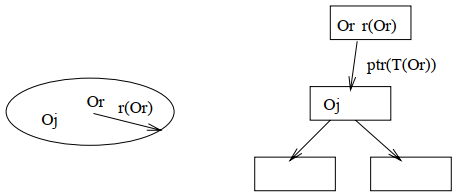
\includegraphics[width=0.55\textwidth]{Figures/mtree.png} % Include the image .png
	\caption{ Un pivot, $ O_r $, avec un rayon de couverture, $  r(O_r) $, qui référence le pivot suivant (sous arbre), $ T(O_r) $.}
\end{figure}

Les feuilles de l’arbre contiennent les identifiants des objets et leurs distances aux pivots associés, les nœuds internes mémorisent plusieurs paramètres comme le pointeur vers le pivot suivant, le rayon de couverture des régions de pivot concernés et un pointeur qui pointe vers le pivot fils. Chaque sous arbre contient les objets qui sont à une distance de pivot $ p $ inferieur au rayon de couverture.\\

\subsection{Comment M-tree grandit?}

Comme tout autre arbre dynamique équilibré (ou balancé), Le processus de construction de M-tree, qui se fait de bas en haut (un mode ascendant buttom-up), parcourt l'arbre à partir de la racine pour insérer le nouvel objet dans le sous arbre qui n'impose pas un changement de rayon de couverture. Si plusieurs sous arbre sont qualifiés, l'objet s'inséra dans le sous arbre de pivot le plus proche à l'objet inséré, sinon l'algorithme cherche le sous arbre qui peut avoir le minimum prolongement pour couvrir le nouvel objet.\\

M-tree est constitué d’un ensemble de nœuds de taille fixe $ M $, si l'insertion d'un objet produit un dépassement de capacité d'un nœud $ N $, le processus de construction fait appel à la fonction Split qui sert à créer un nouveau nœud $ N' $ de même niveau que le nœud saturé $ N  $ et d’appliquer un algorithme de redistribution de $ M+1 $ données entre l’ancien nœud et le nouveau nœud créer. Lorsque la racine se divise, une nouvelle racine est créée et l'arbre $ M $ grandit d'un niveau. La méthode Split est décrite de manière concise comme suit :\\

\begin{figure}[H]
	\centering
	\includegraphics[width=0.95\textwidth]{Figures/split.png} % Include the image .png
\end{figure}

La méthode \textbf{Promote} choisit, en fonction de certains critères spécifiques, deux pivots, $ O_{p1} $ et $  O_{p2} $, à insérer dans le nœud parent, $ N_p $. La partition divise les $ (M + 1) $ entrées du nœud surchargé $ Ne $ en deux sous-ensembles disjoints, $ N_1 $ et $ N_2 $, qui sont ensuite stockés dans les nœuds $ N $ et $ N' $, respectivement. Une mise en œuvre spécifique de \textbf{Promote} et \textbf{Partition} définit ce que nous appelons une stratégie de fractionnement. Contrairement à d'autres modèles d'arbres métriques (statiques), chacun d'entre eux repose sur un critère spécifique d'organisation des objets, M-tree offre la possibilité de mettre en œuvre des stratégies de fractionnement alternatives, qui peuvent être ajustées en fonction des besoins de l'application \textbf{(voir section 3.5.5).}\\

Toute stratégie de fractionnement doit respecter la sémantique du rayon de couverture. Si le nœud du fractionnement, $ N $, est une feuille, cela est garanti par le paramétrage :

\begin{equation}
	r(O_{p1}) = \max \left\{d(O_j, O_{p1}) | O_j \in N_1 \right\}
\end{equation}

En général, le rayon de couverture d'un pivot pointant vers une feuille est égal à la distance maximale entre le pivot lui-même et les objets dans la feuille.\\

Lorsque la division implique un nœud interne, $ N $, chaque entrée $ O_j $ dans $ N_1 $ a un rayon de couverture non nul, $ r(O_j) $. En définissant:

\begin{equation}
r(O_{p1}) = \max \left\{d(O_j, O_{p1}) + r(O_j) | O_j \in N_1 \right\}
\end{equation}

Il est garanti, par la propriété d'inégalité triangulaire, qu'aucun objet dans $ T(O_{p1}) $ ne peut être distant de $  O_{p1} $ plus que $ r(O_{p1}) $. La figure 3.13 le montre dans le cas $ E = ( \mathbb{R^2}, L_2) $, c'est-à-dire le plan réel avec la distance euclidienne.
\begin{figure}[H]
	\centering
	\includegraphics[width=.6 \textwidth]{Figures/splitexep.png} % Include the image .png
	\caption{Fractionnement d'un noeud interne dans l'espace  $ ( \mathbb{R^2}, L_2) $}
\end{figure} 

\subsection{Les requêtes de similarité}
Les algorithmes M-tree pour le traitement des requêtes de similarité visent à réduire le nombre de nœuds accessibles ainsi que le nombre de  de distances calculées. Cela est particulièrement important lorsque la recherche s'avère être orienté CPU, ce qui peut être le cas pour les fonctions de calcul de distance intensives. À cette fin, toutes les distances (pré-calculées) stockées dans les nœuds des M-trees, c'est-à-dire $ d(O_r, P(O_r)) $ et $ r(O_r) $, sont utilisées.

\subsubsection{Les requêtes intervalle (Range Queries)}
La requête $ range(Q, r(Q)) $ sélectionne tous les objets $ O_j $ de la base de données tels que $ d(O_j, Q) \le r(Q) $. L'algorithme \textbf{RangeSearch} part du nœud racine et parcourt récursivement tous les chemins qui ne peuvent pas être exclus pour aboutir à les objets qualifiants.
\begin{figure}[H]
	\centering
	\includegraphics[width=.9 \textwidth]{Figures/rangesearxh.png} % Include the image .png
\end{figure} 

Comme, lors de l'accès au nœud $ N $, la distance entre $ Q $ et $ O_p $, l'objet parent de $ N $, a été déjà calculée, il est possible de se débarrasser d'un sous-arbre sans devoir calculer aucune nouvelle distance. La condition appliquée pour l'élagage (action de débarrasser) est la suivante.
\begin{description}
	\item[Lemme 1 :] Si $ d(O_r, Q) > r(Q) + r(O_r) $, alors, pour chaque objet $ O_j  $ dans $ T (O_r) $, c'est $ d(O_j, Q) > r(Q) $. Ainsi, $ T (O_r) $ peut être éliminé de la recherche en toute sécurité.
\end{description}
En fait, puisque $ d(O_j, Q) \ge d(O_r, Q) - d(O_j, O_r) $ (par l'inégalité triangulaire) et $ d(O_j, O_r) \le r(O_r) $ (par déf. du rayon de couverture), il s'agit de $ d(O_j, Q) \ge d(O_r, Q)-r(O_r) $.
Puisque, par hypothèse, il est $ d(O_r, Q) - r(O_r) > r(Q) $, le résultat suit.
Pour appliquer le Lemme 1, il faut calculer la distance $ d(O_r, Q) $. Cela peut être évité en tirant parti du résultat suivant.
\begin{description}
	\item[Lemme 2 :]  Si $ | d(O_p, Q) - d(O_r, Op) |> r(Q) + r(O_r) $, alors $ d(O_r, Q) > r(Q) + r(O_r) $.
\end{description}

C'est une conséquence directe de l'inégalité triangulaire, qui garantit que $ d(O_r, Q) \ge d(O_p, Q)-d(O_r, O_p) $ et$  d(O_r, Q) \ge d(O_r, O_p)-d(O_p, Q) $ sont tous les deux vrais (voir figure 3.14 en dessous). Le même principe d'optimisation est appliqué aux nœuds feuilles. Les résultats expérimentaux montrent que cette technique permet d'économiser jusqu'à 40\% de calculs de distances [CiPaZe97]. Le seul cas où les distances doivent nécessairement être calculées est celui du nœud racine, pour lequel l'$ O_p $ est indéfini.

\begin{figure}[H]
	\centering
	\includegraphics[width=.6 \textwidth]{Figures/lemme.png} % Include the image .png
	\caption{La figure montre comment le Lemme 2 est utilisé pour éviter de calculer les distances. \\Cas a) : $ d(O_r, Q) \ge d(O_p, Q) - d(O_r, O_p) > r(Q) + r(O_r) $ ; \\
		Cas b) : $ d(O_r, Q) \ge d(O_r, O_p) - d(O_p, Q) > r(Q) + r(O_r) $.}
\end{figure} 

\subsubsection{Les requêtes du k plus proche voisins (k-NN)}

L'algorithme de recherche k-NN (K Nearest Neighbors) récupère les k plus proches voisins d'un objet requête $ Q $ - on suppose qu'au moins $ k $ objets sont indexés par l'arbre M-tree. Nous utilisons une technique de branchement et de liaison(branch-and-bound), assez similaire à celle conçue pour les arbres R-tree [RKV95], qui utilise deux structures globales : une file d'attente prioritaire, \textbf{PR}, et un tableau de k éléments, \textbf{NN}, qui, à la fin de l'exécution, contiendra le résultat.\\

$ PR $ est une file d'attente de pointeurs vers des sous-arbres actifs, c'est-à-dire des sous-arbres où l'on peut trouver des objets qualifiants. Avec le pointeur vers (la racine du) sous-arbre $ T (O_r) $, une limite inférieure, $ d_{min}(T (O_r)) $, sur la distance de tout objet dans $ T (O_r) $ par rapport à $ Q $ est également conservée. La limite inférieure est

\begin{equation}
    d_{\min}(T(O_r)) = \max \left\{d(O_r, Q), 0\right\}
\end{equation}
puisqu'aucun objet dans $ T(O_r) $ ne peut avoir une distance de $  Q  $ inférieure à $ d(O_r, Q)-r(O_r) $.
Ces limites sont utilisées par la fonction \textit{ChooseNode} pour extraire de $ PR $ le noeud suivant à examiner. Comme le critère d'élagage de la recherche k-NN est dynamique - le rayon de recherche est la distance entre $ Q $ et son k-ième voisin le plus proche actuel - l'ordre dans lequel les nœuds sont visités peut affecter les performances. Le critère heuristique mis en œuvre par la fonction \textit{ChooseNode} consiste à sélectionner le nœud pour lequel la limite inférieure de $ d_{min} $ est minimale.(D'après les observations expérimentales, d'autres critères ne conduisent pas à une meilleure performance [CiPaZe97].).
\begin{figure}[H]
	\centering
	\includegraphics[width=.9 \textwidth]{Figures/choosenode.png} % Include the image .png
\end{figure} 


À la fin de l'exécution, la i-ième entrée du tableau $ NN $ aura la valeur $ NN[i] = [oid(O_j),d(O_j, Q)] $, $ O_j $ étant le i-ième voisin le plus proche de $ Q $. La valeur de la distance dans la i-ième entrée est désignée par $ d_i $, de sorte que $ d_k $ est la plus grande valeur de distance dans $ NN $. Il est clair que $ d_k $ joue le rôle d'un rayon de recherche dynamique, puisque tout sous-arbre pour lequel $ d_{min}(T(O_r)) > d_k $ peut être \textbf{élagué} en toute sécurité.\\

Les entrées du tableau $ NN $ sont initialement fixées à $ NN[i] = [null ,\infty] (i= 1,..., k) $, c'est-à-dire que les $ oid $ sont indéfinis et $ d_i = \infty $. Lorsque la recherche commence et que l'on accède aux nœuds (internes), l'idée est de calculer, pour chaque sous-arbre $ T(O_r) $, une limite supérieure, $ d_{max}(T(O_r)) $, sur la distance de tout objet dans $ T(O_r) $ par rapport à $ Q $. La limite supérieure est fixée à

\begin{equation}
d_{\max}(T(O_r)) =  d(O_r, Q)+r(O_r)
\end{equation}

Considérons le cas le plus simple $ k = 1 $, deux sous-arbres, $ T(O_{r1}) $ et $ T(O_{r2}) $, et supposons que $ dmax(T(O_{r1})) = 5 $ et $ dmin(T(O_{r2})) = 7 $. Puisque $ d_{max}(T(O_{r1})) $ garantit qu'un objet dont la distance de $  Q $ est au plus égale à 5 existe dans $ T(O_{r1}) $, $ T(O_{r2}) $ peut être élagué de la recherche. Les limites $ d_{max} $ sont insérées à des positions appropriées dans le tableau $ NN $, laissant juste le champ $ oid $ non défini. L'algorithme de recherche $ k-NN $ est donné ci-dessous.
\begin{figure}[H]
	\centering
	\includegraphics[width=.9 \textwidth]{Figures/knnsearch.png} % Include the image .png
\end{figure} 

La méthode \textit{k-NN-NodeSearch} implémente la majorité de la logique de recherche. Sur un nœud interne, elle détermine d'abord les sous-arbres actifs et les insère dans la file d'attente $ PR $. Ensuite, si nécessaire, elle appelle la fonction \textit{NN-Update} pour effectuer une insertion ordonnée dans le tableau $ NN $ et reçoit en retour un (possiblement nouvelle) valeur de $ d_k $. Cette valeur est ensuite utilisée pour retirer de $ PR $ tous les sous-arbres pour lesquels la limite inférieure de $ d_{min} $ dépasse $ d_{k} $. Des actions similaires sont effectuées dans les nœuds feuilles. Dans les deux cas l'optimisation visant à réduire le nombre de calculs de distance, qui utilise les distances pré-calculées de l'objet parent, est appliquée.

\begin{figure}[H]
	\centering
	\includegraphics[width=.9 \textwidth]{Figures/knnnodesearch.png} % Include the image .png
\end{figure} 

\subsection{Insertion d'objets}
L'algorithme d'insertion descend récursivement l'arbre MT pour localiser le nœud feuille le plus approprié pour accueillir un nouvel objet, $ O_n $, déclenchant éventuellement une division si la feuille est pleine. Le raisonnement de base pour déterminer le nœud feuille "le plus approprié" est de descendre, à chaque niveau de l'arbre, le long d'un sous-arbre, $ T(O_r) $, pour lequel aucun élargissement du rayon de couverture n'est nécessaire, c'est-à-dire$  d(O_r, O_n) \le r(O_r) $. S'il existe plusieurs sous-arbres ayant cette propriété, on choisit celui pour lequel l'objet $ O_n $ est le plus proche de $ O_r $. Ce critère heuristique tente d'obtenir des sous-arbres bien regroupés, ce qui a un effet bénéfique sur les performances.\\

Si aucun pivot pour lequel $ d(O_r, O_n) \le r(O_r) $ existe - donc un rayon de couverture doit être élargi - notre choix est de minimiser l'augmentation du rayon de couverture, c'est-à-dire $ d(O_r, O_n)-r(O_r) $. Ceci est étroitement lié au critère heuristique qui suggère de minimiser le "volume" global couvert par les pivots dans le nœud actuel. L'algorithme Insert résume les arguments ci-dessus.
\begin{figure}[H]
	\centering
	\includegraphics[width=.9 \textwidth]{Figures/insert.png} % Include the image .png
\end{figure} 


\subsection{Stratégies de fractionnement}
La stratégie de fractionnement "idéale" devrait sélectionner les deux objets à promouvoir, $ O_{p1} $ et $ O_{p2} $, et répartir les entrées de telle sorte que les deux régions ainsi obtenues aient un "volume" minimum et un "chevauchement" minimum. Ces deux critères visent à améliorer l'efficacité des algorithmes de recherche, car le fait d'avoir des régions de petite taille (faible volume) conduit à des arbres bien groupés et réduit la quantité d'espace inactif indexé - espace où aucun objet n'est présent - et le fait que le chevauchement entre les régions soit faible (voire nul) réduit le nombre de chemins à parcourir pour répondre à une requête.\\

Le critère du volume minimum conduit à concevoir des stratégies de fractionnement qui tentent de minimiser les valeurs des rayons de couverture, tandis que l'exigence de chevauchement minimum suggère que, pour des valeurs fixes des rayons de couverture, la distance entre les deux objets de référence choisis devrait être maximisée.

\subsubsection{Choix des pivots}
La méthode Promote détermine, à partir d'un ensemble d'entrées, $ Ne $ , deux objets à promouvoir et à stocker dans le nœud parent (voir section 3.5.2). Les algorithmes spécifiques que nous considérons peuvent d'abord être classés selon qu'ils "confirment" ou non l'objet parent dans son rôle.

\begin{description}
	\item[Définition]  Une stratégie de fractionnement confirmée choisit l'un des deux objets à promouvoir, par exemple l'$ O_{p1} $, pour être l'objet parent lui-même, $ O_p $, du nœud de fractionnement.
\end{description}

En d'autres termes, une stratégie de fractionnement confirmée ne fait que "extraire" une région, centrée sur le deuxième Pivot, l'$ O_{p2} $, de la région qui restera centrée sur l'$ O_p $. En général, cela simplifie l'exécution du fractionnement et réduit le nombre de calculs de distance.\\

Les alternatives que nous décrivons pour la mise en œuvre de Promote ne sont qu'un sous-ensemble sélectionné de l'ensemble que Ciaccia, Patella, Rabitti et Zezula ont évalué expérimentalement. Les autres stratégies sont décrit dans [CiPaZe97].

\begin{itemize}
	\item \textbf{m\_RAD :} L'algorithme du "minimum (sum of) RADius" est le plus complexe en termes de calcul de la distance. Il prend en compte toutes les paires d'objets possibles et, après avoir partitionné l'ensemble des entrées, promeut la paire d'objets pour laquelle la somme des rayons de couverture, $ r(O_{p1}) + r(O_{p2}) $, est minimale.
	\item \textbf{RANDOM :} Cette variante sélectionne simplement de manière aléatoire le ou les objets de référence.
	Bien que cette stratégie ne semble pas "intelligente", elle est rapide et ses performances peuvent servir de référence pour d'autres stratégies.
	\item \textbf{SAMPLING :} C'est la stratégie RANDOM, mais elle a été répétée sur un échantillon d'objets de taille $ s > 1 $. Pour chacune des paires d'objets $ s(s - 1)/2 $ de l'échantillon, les entrées sont réparties et des rayons de couverture potentiels sont établis. La paire pour laquelle la somme résultante des rayons de couverture, $ r(O_{p1})+r(O_{p2}) $, est minimale est alors sélectionnée.
	En cas de promotion confirmée, seules $ s $ différentes distributions sont essayées. Dans les expériences de [CiPaZe97], la taille de l'échantillon a été fixée à $ 1/10 $-ème de la capacité des nœuds.
	\item \textbf{M\_LB\_DIST :} L'acronyme signifie "Maximum Lower Bound on DISTance".
	Cette stratégie diffère des précédentes en ce sens qu'elle n'utilise que les distances stockées pré-calculées. Dans la version confirmée, où $ O_{p1} \equiv O_p $, l'algorithme détermine que l'$ O_{p2} $ est l'objet le plus éloigné de l'$ O_p $, c'est-à-dire:
	\begin{equation}
		 d(O_{p2}, O_p) = \max_j{d(O_j, O_p)}
	\end{equation}
	Lorsque $ O_{p1} = O_p $, les deux objets promus sont choisis de manière à ce que:
	\begin{equation}
	\makecell{d(O_{p1}, O_p) = \min_j{d(O_j, O_p)} \\
		 d(O_{p2}, O_p) = \max_j{d(O_j, O_p)}}
	\end{equation}
	La distance entre les deux pivots est alors garantie d'être au moins\\ $ d(O_{p2}, O_p)-d(O_{p1}, O_p) $, et aucun autre choix ne peut conduire à une limite supérieure.
\end{itemize}
Dans notre système nous avons choisi la dernière mèthode qui est M\_LB\_DIST.

\subsubsection{Répartition des entrées}
Étant donné un ensemble d'entrées $ Ne $ et les deux pivots $ O_{p1} $ et $ O_{p2} $, le problème est de savoir comment partitionner efficacement $ Ne $ en deux sous-ensembles, $  N_1 $ et $ N_2 $. À cette fin, nous envisager deux stratégies de base. La première est basée sur l'idée de la décomposition généralisée de l'hyperplan [Uhl91] et conduit à des fractionnements déséquilibrés, alors que la second obtient une répartition équilibrée. Ils peuvent être brièvement décrits comme suit.
\begin{itemize}
	\item \textbf{Hyperplan généralisé (Generalized Hyperplane) :} Assignez chaque objet $ O_j \in Ne $ au  pivot le plus proche, c'est-à-dire si $ d(O_j, O_{p1}) \le d(O_j, O_{p2}) $ alors assignez $ O_j $ à $ N_1 $, sinon assignez $ O_j $ à $ N_2 $.
	
	\item \textbf{Équilibré (Balanced) :} Calculer $ d(O_j, O_{p1}) $ et $ d(O_j, O_{p2}) $ pour tous les $ O_j \in Ne $ Répéter jusqu'à ce que $ Ne $ soit vide :\\
	 - Affecter à $ N_1 $ le plus proche voisin de l'$ O_{p1} $ dans $ Ne $ et le retirer de $ Ne $ ;\\
	 - Attribuer à $ N_2 $ le plus proche voisin de l'$ O_{p2} $ dans $ Ne $ et le retirer de $ Ne $.
\end{itemize}
En fonction de la distribution des données et de la manière dont les objets de routage sont choisis, une stratégie de fractionnement déséquilibrée peut conduire à un meilleur partitionnement des objets, en raison du degré de liberté supplémentaire que l'on obtient. En particulier, il faut remarquer que, si l'obtention d'un fractionnement équilibré avec des méthodes d'accès spatiale oblige à n'élargir les régions que selon les dimensions nécessaires, dans un espace métrique, l'augmentation conséquente du rayon de couverture se propagerait à toutes les "dimensions".\\

Un comportement intermédiaire peut être obtenu en combinant les deux algorithmes ci-dessus et en fixant un seuil minimum d'utilisation des nœuds. Si au moins $ m \le M/2 $ entrées par nœud sont nécessaires, la distribution équilibrée peut être appliquée aux 2 premiers $ m $ objets, après quoi l'hyperplan généralisé pourrait être utilisé. 

Pour en savoir plus sur l'évaluation des pérformances de la structures M-tree avec ses différentes types de requêtes et stratégies de fractionnement (partitionnement) le lecture peut consulter l'article [CiPaZe97].

\section{Conclusion}
Dans ce chapitres nous avons fait une études non exhaustive des méthodes d'indexations et leurs classifications. Pricipalement, nous avons présenté la structure d'accès métrique M-Tree et comment elle est construite, ainsi que ses algorithmes d'insertion et de recherche.

Généralement, la structure M-tree présente des avantages suivants: coût de recherche diminuer, dynamique, et résistance à l’augmentation de
la dimension. Mais, il peut présenter des chevauchement des nœuds [Hanif18].\\


Dans ce qui suit nous présenterons notre systèmes de recherche d'images par le contenu.

%
%
%
%La recherche par la requête intervalle R(q,r) d’un objet requête q et de rayon r dans M-tree exploite les distances pré-calculer pour éviter le parcours des nœuds inutiles. En effet, le processus de recherche commence par la racine, et pour chaque nœud visité: si la condition
%$ |d(q,p^p) — d(pp,^p)| — r^c > r $ est vérifiée alors on peut éviter le parcours du nœud sans faire des calculs supplémentaires, tel que $ d(q,p^p) $ est la distance entre la requête et l’objet père du nœud , $ d(p^p,p) $ est la distance entre l’objet p et l’objet père du nœud et $ r^c $ le rayon de couverture de nœud.
%
%La complexité de la construction de M-tree est d’ordre$  O(n.m^2.log_m n) $ telle que n est lenombre des distances stockées dans les feuilles et m représente la taille maximale des nœuds.


%P. Ciaccia, M. Patella, F. Rabitti, P. Zezula Indexing Metric Spaces with M-tree
%% Chapter Template

\chapter{Implémentation et évaluation expérimentale} % Main chapter title

\label{Chapter4} % Change X to a consecutive number; for referencing this chapter elsewhere, use \ref{ChapterX}

%----------------------------------------------------------------------------------------
%	SECTION 1
%----------------------------------------------------------------------------------------

\section{Introduction}
Après avoir étudié le domaine de CBIR (les systèmes de recherche d’images par le contenu ) et leur principe de fonctionnement, l’implémentation d’une application ou d’un système de recherche d’images par le contenu devient une nécessité afin d’avoir une vue plus claire de ce que nous avons introduit dans les premiers chapitres. \\

Nous présenterons alors, dans ce chapitre, notre application,
les descripteurs utilisés et les bases d’images choisies afin de pouvoir évaluer le système, ainsi les différentes étapes par lesquelles nous sommes passés pour sa réalisation.

\section{L'outil d’implémentation}
Dans la conception de notre application, nous avons choisi Python
comme langage de programmation, ce choix est justifié par plusieurs
facteurs, parmi eux on cite:
\begin{itemize}
	\item Une librairie très riche, il est complété par de multiples boîtes à outils (le calcul numérique matriciel avec Numpy, vision par ordinateur avec OpenCV, ...etc).
	\item Une syntaxe simple permettant une souplesse durant l'implémentation.
	\item Possible d’exécuter le code en dehors du programme (Testes unitaires).
	\item Une aide très bien faite.
	\item Opensource contrairement à Matlab.
\end{itemize}

\begin{figure}[H]
	\centering
	\includegraphics[width=0.3\textwidth]{python}
	\caption{Exemple de librairies Python.}
\end{figure}

\section{Les descripteurs d’image utilisés}
La première étape de création d'un système CBIR est le choix d'un descripteur pour indexer les images. \\
Pour la création de notre vecteur descripteur (signature), nous avons utilisé des caractéristiques de bas niveau comme déjà spécifier dans le chapitre 2. L'extraction se fait selon l'attribut visuel choisi: couleur, texture ou forme.
\subsection{Les descripteurs de couleur}
\textbf{Les modèles de couleur: }
Dans notre système, nous avons intégré l'espace RGB et l'espace TSV (HSV):\\

\begin{itemize}
	\item Le modèle TSV (Teinte Saturation Valeur) : est une représentation physique de la couleur, cet espace présente l’avantage de simuler le comportement visuel humain.
	
	\item Le modèle RVB (Rouge, Vert, Bleu) : est l’espace de couleur le plus utilisé pour la représentation de la couleur. L’avantage d’utiliser ce modèle est que cette représentation est extrêmement basique, puisqu’aucun traitement n’est nécessaire.\\
	
\end{itemize}

Notre système présente à l'utilisateur les descripteurs suivants :
\begin{itemize}
	\item L'histogramme (RGB et HSV),
	\item Les moments statistiques.
\end{itemize}

\subsubsection{Histogramme}
\paragraph{RVB (RGB):}
Dans la création de l’application, nous avons choisi d’utiliser les histogrammes par bloc dans l’espace RVB comme une technique de base comme spécifier dans l'article [Abed15].
On a choisi de diviser l'histogramme en 17 blocs pour chaque composante; Rouge, Verte et Bleu. Le vecteur de caractéristiques $ V_{histRGB} $ est généralement de taille 17x17x17 = 4913.
\begin{table}[H]
	\centering
	\caption{Exemple d'histogramme par blocs}
	\begin{tabular}{|c|c|c|c|c|c|}
		\hline
		\textbf{Block} & \textbf{Fréquence} & \textbf{Block} & \textbf{Fréquence} & \textbf{Block} & \textbf{Fréquence}\\
		\hline
		
		\makecell{0-15 } & \makecell{454 } & \makecell{16-30 } & \makecell{2324 }   & \makecell{31-45 } & \makecell{345 }   \\
		\hline
		
		\makecell{46-60 } & \makecell{903 } & \makecell{61-75 } & \makecell{133 }   & \makecell{76-90 } & \makecell{563 }   \\
		\hline
		
		\makecell{91-105 } & \makecell{123} & \makecell{106-120 } & \makecell{67 }   & \makecell{121-135 } & \makecell{124 }   \\
		\hline
		
		\makecell{136-150 } & \makecell{856} & \makecell{151-165 } & \makecell{45 }   & \makecell{166-180 } & \makecell{454 }   \\
		\hline
		
		\makecell{181-195 } & \makecell{355} & \makecell{196-210} & \makecell{31}   & \makecell{211-215 } & \makecell{4546 }   \\
		\hline
		
		\makecell{216-230 } & \makecell{456} & \makecell{231-255} & \makecell{3456}   & \makecell{  } & \makecell{  }   \\
		\hline
	\end{tabular}
	
	
\end{table}
\paragraph{TSV (HSV):}
Pour notre moteur de recherche d'images, nous utiliserons un histogramme couleur 3D dans l'espace couleur HSV avec 8 blocs pour le canal teinte, 12 blocs pour le canal saturation et 3 blocs pour le canal valeur en divisant l'image en 5 régions, ce qui donne un vecteur de caractéristiques $ V_{histHSV} $ est de  dimension 8 x 12 x 3 x 5 = 288 x 5 = 1440.
\begin{figure}[H]
	\centering
	\includegraphics[width=0.3\textwidth]{5regions}
	\caption{Exemple de division d'une image en 5 régions différentes [Site01].}
\end{figure}
\subsubsection{Les moments de couleur}
Pour enrichir les index de la couleur, nous avons utilisé les moments de couleur au lieu de calculer la distribution complète comme pour les histogrammes. Dans cette étape, nous avons calculé les trois premiers moments de couleur (la moyenne, l’écart-type et le moment d'ordre 3) pour chaque canal (R,G,B) dans le but de garder seulement les neuf valeurs obtenues, ainsi le vecteur de caractéristiques $ V_{moments} $ est de tailles 9.

\subsection{Les descripteurs de texture}
Pour caractériser la texture, nous avons choisi l'un des descripteurs classiques à savoir les mesures de Haralick basé sur les matrices de co-occurrence. De plus, nous avons intégré les filtres de Gabor comme étant l'un des descripteurs fortement utilisés dans la littérature.
\subsubsection{Les mesures de Haralick}
Les mesures de Haralick sont calculées à partir de la matrice de co-occurrence de l'image. Haralick décrit 14 statistiques qui peuvent être calculées à partir de la matrice de co-occurrence dans le but de décrire la texture de l'image [Site02]. Nous adoptant l'implémentation de la librairie Mahotas [Site03] qui met en œuvre seulement les 13 premières mesures. La dernière (14ème) est normalement considérée comme instable. Alors, le vecteur de caractéristiques $ V_{Haralick} $ est de taille 13.

\subsubsection{Les filtres de Gabor}
Dans le but d'améliorer les performances lié à la recherche basé sur la texture, nous avons utilisé les filtres de Gabor vue leurs robustesse prouvé par de nombreuse travaux de recherche dans la littérature [ElHasnaoui17] et [ZZ18].\\

En traitement d'images, un filtre de Gabor, nommé d'après Dennis Gabor, est un filtre linéaire utilisé pour l'analyse de la texture:

\begin{equation}
g(x,y;\lambda,\theta,\psi,\sigma_x,\sigma_y) = \frac{1}{2\pi \sigma_x \sigma_y} \exp\left(\frac{-x'^2}{\sigma_x^2} + \frac{y'^2}{\sigma_y^2}\right)\exp\left(i\left(2\pi\frac{x'}{\lambda}+\psi\right)\right) 
\end{equation}
Où: $ x' = x \cos\theta + y \sin\theta\, $, $ y' = -x \sin\theta + y \cos\theta\, $, \\
$\psi$ : La phase, \\
$\theta$ : la direction, \\
et $ \lambda $: la fréquence.\\

Les filtres d'ondelettes de Gabor s'étendent sur 5 fréquences : 0.06, 0.09, 0.13, 0.18, 0.25 avec huit orientations $ \theta_0 = 0, \theta_n = \theta_{n-1} + \frac{\pi}{8} , n = 1,...,7$  et qui sont appliqués sur l'image. La moyenne et l'écart-type des coefficients d'ondelettes de Gabor des images résultante sont utilisés pour former un vecteur de caractéristiques $ V_{Gabor} $ de taille 5x8x2 = 240.

\subsection{Les descripteurs de forme}
Dans la partie basé sur la forme, nous avons intégré les moments de Hu comme descripteur classique et les moments de Zernike qui constitue une amélioration de performance comparant au moment de Hu.
\subsubsection{Moments de Hu}
Les moments de Hu sont basés sur les moments géométriques discutés dans le chapitre II section 2.2.3.\\
Si ƒ(x, y) est une image numérique, alors l'équation précédente devient:
\begin{equation}
\mu_{p,q} = \sum_{x=0}^{M-1}\sum_{y=0}^{N-1} (x- \bar{x})^p (y-\bar{y})^q f(x, y)
\end{equation}
D'où les moments géométriques (centraux):
\begin{figure}[H]
	\includegraphics[width=0.5\textwidth]{momentCent} \includegraphics[width=0.5\textwidth]{momentCent1}
\end{figure}
Où:
\begin{equation}
\begin{tabular}{cc}
$\bar{x} = \frac{M_{1,0}}{M_{0,0}}$ & $\bar{y} = \frac{M_{0,1}}{M_{0,0}}$
\end{tabular}
\end{equation}
Les moments $ \mu_{p,q} $ invariants en ce qui concerne à la fois la translation et l'échelle peuvent être construits à partir des moments géométriques en divisant par un moment central zéro-ième correctement mis à l'échelle :
\begin{equation}
\eta _{{ij}}={\frac  {\mu _{{ij}}}{\mu _{{00}}^{{\left(1+{\frac  {i+j}{2}}\right)}}}}\,\!
\end{equation}
où $ i + j \ge 2 $.
Comme le montre le travail de Hu, [Hu62] les invariants en matière de translation, d'échelle et de rotation peuvent être construits :
\begin{figure}[H]
	\centering
	\includegraphics[width=1\textwidth]{huMom}
	\caption{Les moments de Hu.}
\end{figure}

Le vecteur de caractéristiques $ V_{Hu} $ est alors de taille 7.
\subsubsection{Moments de Zernike}
En 1934, Zernike [Site05] [MYB07] a proposé un ensemble de polynômes orthogonaux définis sur le cercle unité, à savoir les polynômes orthogonaux de Zernike, leur formule de définition est la suivante :
\begin{equation}
V_{mn}(x, y)~=~V_{mn}(r,\theta)~=~R_{mn}(r)\exp(jn\theta)
\end{equation}
où:
\begin{displaymath}
R_{mn}(r) = \sum_{s=0}^{\frac{m-\mid n \mid}{2}}(-1)^{s}~~F(m,n,s,r)
\end{displaymath}
\begin{displaymath}
F(m,n,s,r) = \frac{(m-s)!}{s!(\frac{m+\mid n \mid}{2}~-s)!~(\frac{m-\mid n \mid}{2}~-s)! }~r^{m-2s}
\end{displaymath}
$ R_{mn}(r) $  est le polynôme radial orthogonal, $ V_{mn}(x, y) $ est le polynôme orthogonal de Zernike, c'est un ensemble de fonctions orthogonales à valeurs complexes avec complétude définies sur le disque unité $x^{2} + y^{2} \leq ~1$ , n et m sont les ordres des polynômes orthogonaux de Zernike, où n est un entier positif ou zéro, m est un entier positif ou négatif, ils sont soumis aux conditions 
\begin{equation}
m- \mid n \mid ~=~pair~~,~~\mid n \mid~\leq~m
\end{equation}

\paragraph{Définition des Moments de Zernike:}
En 1980, sur la base des polynômes orthogonaux de Zernike, Teague a proposé pour la première fois la définition des moments de Zernike d'une fonction d'image f( x, y) en deux dimensions
\begin{equation}
Z_{mn} = \frac{m+1}{\pi} \int_{x} \int_{y} f(x,y)[V_{mn}(x,y)]^{*} ~dx~dy~~~~~\mbox{where $x^{2} + y^{2} \leq ~1$}
\end{equation}
où $m = 0,1,2,...,\infty$ et définit l'ordre, $f(x,y)$ est la fonction décrite et $*$ désigne le conjugué complexe. Alors que $n$ est un nombre entier (qui peut être positif ou négatif) décrivant la dépendance angulaire, ou rotation, sous conditions (4.4). Pour les images numériques, les intégrales sont remplacées par des sommations, alors les moments de Zernike sont réécrits comme :

\begin{equation}
Z_{mn} = \frac{m+1}{\pi} \sum_{x} \sum_{y} P_{xy}[V_{mn}(x,y)]^{*} ~~~~~\mbox{where $x^{2} + y^{2} \leq ~1$}
\end{equation}
Dans la littérature on trouve d'autres variants ou améliorations des moments de Zernike. Pour nous, on a adopter l'implémentation de la librairie Mahotas pour nous simplifier la vie. On générale, il faut fixer un rayon centré sur le centre de masse de l'image (le rayon du cercle enveloppant minimal de la forme).
Le vecteur de caractéristiques $ V_{Zernike} $ et de taille 25.

\subsection{Combinaison des descripteurs}
Les attributs: couleur, texture, forme décrivent les images par leur contenu visuel. La combinaison de ces attributs peut caractériser mieux le contenu. Il est donc intéressant de
combiner ces différents attributs pour une recherche plus efficace et plus discriminante. Les problèmes qui se posent lors de la combinaison de ces différents attributs pour la recherche et l’indexation sont au moins de trois ordres :

\begin{itemize}
	\item  \textbf{L'espace de description} : Le choix de l'espace de description consiste à rechercher les attributs visuels significatifs de la base de données d'images, l'ensemble de ces
	attributs étant représenté par un nuage de points dans un espace dimensionnel haut, alors les vecteurs contiennent plusieurs attributs, un problème qui se pose est celui de la dimension de l'espace de description. Ce problème est connu dans la communauté
	des bases de données par la malédiction de la dimension, lorsque le nombre de dimensions augmente, le volume de l'espace croît rapidement si bien que les données se retrouvent isolées et deviennent éparses.
	
	\item \textbf{ La mesure de la similarité} : Il s'agit d'une étape essentielle dans tout système de
	recherche. Dans le cas où les images sont décrites par différents attributs, une solution
	classique pour mesurer la similarité est de calculer séparément les mesures de
	similarité pour chaque attribut et de déduire ensuite une mesure composite de la
	similarité globale entre les images. Cela suppose évidemment que les différents
	attributs sont indexés séparément (avec des structures d'index séparées). Dans la base
	de données, il y a peu de méthodes qui utilisent plusieurs index pour structurer les
	données. Une autre difficulté liée à la similitude est de déterminer comment combiner
	plusieurs mesures souvent définies sur des domaines différents, avec des dynamiques
	différentes, des degrés d'importance différents, surtout pour l'utilisateur, mais aussi de
	natures différentes.
	
	\item \textbf{Structuration} : la phase de construction d'une structure d'index est une étape utile dans
	le cas où les données sont volumineuses et appartiennent à un grand espace de
	description. Il s'agit de structurer les nuages de points relatifs aux descripteurs des
	images et de les stocker efficacement dans une machine. Cette tâche de structuration
	peut s'avérer difficile dans le cas où les données à structurer sont de nature hétérogène.
	La difficulté réside dans le choix de la distance à utiliser pour structurer (mise en place
	d'un index) et dans la standardisation des différents types de données.
\end{itemize}
\subsubsection{La couleur et la texture}
Pour diminuer la taille du vecteur descripteur (signature) autant que possible nous avons choisi d'utiliser les moments de couleur, qui produit une signature de taille 9, pour caractériser la couleur. En ce qui concerne la caractérisation de la texture on travaille avec les filtres de Gabor.
\begin{figure}[H]
	\centering
	\includegraphics[width=0.6\textwidth]{clrtxtr}
	\caption{Dérivation de signature couleur et texture.}
\end{figure}
Où: 
M: Moyenne, E: Ecart-type, T: moment d'ordre trois.
\begin{equation}
V_{final} = V_{moments} \bigcup V_{Gabor}
\end{equation}
\subsubsection{La couleur et la forme}
Nous utilisons les moments de couleur pour les mêmes raisons pour caractériser la couleur. En ce qui concerne la caractérisation de la forme on travaille avec les moments de Zernike car l'expérience preuve qu'il sont plus performant que les moments de Hu.
\begin{figure}[H]
	\centering
	\includegraphics[width=0.6\textwidth]{clrshp}
	\caption{Dérivation de signature couleur et texture.}
\end{figure}
Où: 
$ M_i $: Moment i.
\begin{equation}
V_{final} = V_{moments} \bigcup V_{Zernike}
\end{equation}

Pour fusionner les différents descripteurs, une méthode utilisée dans différents travaux [ElAsnaoui17] consiste à pondérer les distances de similarité. Ainsi les descripteurs pertinents pour la recherche se verront attribuer des poids les plus importants, et auront donc plus d’influence dans le résultat final. La combinaison des distances est donnée par la relation suivante :
\begin{equation}
	D_{global}(Q, I) = w_1 \times 	D_{1}(Q, I) + w_2 \times 	D_{2}(Q, I)
\end{equation}
où $ w_i $ est un poids qui prend une valeur entre 0 et 1 avec $ w_1+w_2= 1 $.
\section{Mesures de similarité}
La deuxième étape dans les systèmes de recherche d'image par le contenu est le choix d'une mesure de similarité pour effectuer la recherche.\\

Pour rechercher les images les plus similaires à une image requête, il faut pouvoir mesurer la similarité entre les images. Lorsqu’un utilisateur lance une recherche, le système effectue une mesure entre le signature de la requête et les signatures des images de la base dans l’espace des attributs (signatures).\\

D'une façon générale, nous avons choisi d’utiliser les distances dérivées de la famille de distances de Minkowski; la distance de Manhatan et la distance Euclidienne.\\

Pour les distributions statistiques à savoir les histogrammes, nous avons ajouter les distances:  $\chi^2$ (CHI-square) et Bhattacharyya  .

\begin{table}[H]
	\centering
	\caption{Les distances de Minkowski}
	\begin{tabular}{|c|c|c|}
		\hline
		\textbf{Distance} & \textbf{Formule}\\
		\hline
		\makecell{Manhatttan } & \makecell{\\
			$  d_1(I_1, I_2) = \sum_{i=1}^{N} \left|{I}_{1}(i)-{I}_{2}(i)\right|  $ }   \\
		\hline
		
		\makecell{Euclidienne} & \makecell{\\ $ d_2(I_1, I_2) =  \sqrt{\sum_{i=1}^{N} \left|{I}_{1}(i)-{I}_{2}(i)\right|^2} $}   \\
		\hline
		
		\makecell{$\chi^2$ (CHI-square)  } & 
			\makecell{\\
				$d(I_1, I_2)=\sum_{i=1}^{N} \frac{(I_1(i)-I_2(i))^2}{I_1(i)}$
			} \\   
		\hline
		
		\makecell{Bhattacharyya } & 
		\makecell{\\
			$d(I_1, I_2) ~=~ \sqrt{ 1 - \frac{1}{ \sqrt{\bar{I_1}\bar{I_2} N^2} }  \sum_{i=1}^{N} \sqrt{I_1(i)\times I_2(i)}}$
		} \\   
		\hline
		
		
	\end{tabular}
	
\end{table}
Ou :\\
$ I_1, I_2 $ sont les deux vecteurs de caractéristiques.\\
$ N $ est la dimension de vecteur.\\
$ i $ indice.
$ bar{I_i} $ la moyenne.

\section{Les bases d’mages utilisées }
\textbf{Corel-1000 - Wang:}
Cette base d’images contient 1000 images en couleurs. Ces images ont
été divisées en 10 classes de 100 images. Les thèmes représentés par les 10 classes sont : monuments, plage, autobus, dinosaures, aliments, éléphants, fleurs, chevaux, montagnes et l’Afrique.

\begin{figure}[H]
	\centering
	\includegraphics[width=0.6\textwidth]{wang} 
	\caption{Quelques images de la base d’image WANG.}
\end{figure}

\textbf{Columbia Object Image Library (COIL-100):}
Cette base d’images est très connue pour la reconnaissance des objets. Il y a deux bases d’images COIL : COIL-20 qui contient des images en niveaux de gris prises à partir de 20 objets différents et COIL-100 qui contient des images en couleurs prises à partir de 100 objets différents. Les deux bases d’images consistent en des images prises à partir des objets 3D avec des positions différentes. La base COIL-100 a 7200 images en couleurs (100 objets x72 images/objet). Chaque image a une taille de 128x128 pixels.

\begin{figure}[H]
	\centering
	\includegraphics[width=0.6\textwidth]{coil} 
	\caption{Objets utilisés dans COIL-100.}
\end{figure}

\textbf{Columbia-Utrecht Reflectance and Texture Database (CuRRET):}
Des chercheurs des universités de Columbia et d'Utrecht ont collaboré dans une étude approfondie de l'aspect visuel des surfaces du monde réel. Cet effort conjoint, parrainé en partie par REALISE de la Commission européenne, la National Science Foundation et par le DARPA/ONR dans le cadre de la subvention MURI n° N00014-95-1-0601, a donné lieu à 3 bases de données [Site04]. Nous avons choisi 33 échantillons parmi 61 échantillons avec 50 images par échantillon.
\begin{figure}[H]
	\centering
	\includegraphics[width=0.5\textwidth]{curet} 
	\caption{Quelques images de la base d’image CurRRET.}
\end{figure}

%\textbf{MIT1995 - VisTex:}
%La base de données VisTex est une collection d'images de texture. La base de données a été créée dans le but de fournir un large ensemble de textures de haute qualité pour les applications de vision par ordinateur. En particulier, l'ensemble a été conçu comme une alternative à la bibliothèque de textures Brodatz, qui n'est pas disponible gratuitement pour la recherche [Site01]. L'objectif de VisTex est de fournir des images de texture qui sont représentatives des conditions du monde réel. Si VisTex peut remplacer les collections de textures traditionnelles, il comprend des exemples de nombreuses textures non traditionnelles. La base de données comporte plus de 100 images.
%
%\begin{figure}[h]
%	\centering
%	\includegraphics[width=0.6\textwidth]{VisTex} 
%	\caption{Quelques images de la base d’image VisTex.}
%\end{figure}
%
%\textbf{MIT1995 - TRUNK12:}
%Comme il n'existe pas d'ensemble de données d'images d'écorces d'arbres connu et accessible au public, un nouvel ensemble de données accessible au public a été créé dans le cadre de la thèse de Bsc [Site02]. Il contient environ 360 images d'écorces de 12 arbres différents qui se trouvent en Slovénie. Chaque classe d'arbres comprend environ 30 images au format JPEG, avec une résolution de 3000 x 4000 pixels. Toutes les images ont été prises avec l'appareil photo Nikon COOLPIX S3000 dans les mêmes conditions (distance de 20 cm, plusieurs arbres par classe, en évitant le bruit comme la mousse, mêmes conditions de lumière, prises en position verticale).
%
%\begin{figure}[H]
%	\centering
%	\includegraphics[width=0.6\textwidth]{trunk} 
%	\caption{Quelques images de la base d’image TRUNK12.}
%\end{figure}

\section{Mesure de la qualité des réponses}
Dans les systèmes de recherche d’images, une image est pertinente pour
une requête si les deux images sont dans la même classe.
La précision (ou valeur prédictive positive) est la proportion des items pertinents parmi l'ensemble des items proposés; le rappel (ou sensibilité) est la proportion des items pertinents proposés parmi l'ensemble des items pertinents. Ces deux notions correspondent ainsi à une conception et à une mesure de la pertinence.\\

Lorsqu'un moteur de recherche, par exemple, retourne 30 pages web dont seulement 20 sont pertinentes (les vrais positifs) et 10 ne le sont pas (les faux positifs), mais qu'il omet 40 autres pages pertinentes (les faux négatifs), sa précision est de 20/30 = 2/3 et son rappel vaut 20/(20+40) = 1/3.\\

La précision peut ainsi être comprise comme une mesure de l'exactitude ou de la qualité, tandis que le rappel est une mesure de l'exhaustivité ou de la quantité.\\


\begin{figure}[H]
	\includegraphics[width=0.5\textwidth]{recpre} 
	\includegraphics[width=0.5\textwidth]{recallprecision} 
	\caption{Rappel et précision comme illustré par Wikipédia.}
\end{figure}
Le rappel et la précision sont deux mesures très utilisées pour l’évaluation des performances d’un système CBIR. 

\begin{equation}
R = \frac{\text{VP}}{\text{FN et VP}} = \frac{\text{Nombre d'images pértinentes retrouvées} }{\text{Nombre total d'images pértinentes}}
\end{equation}
\begin{equation}
P = \frac{\text{VP}}{\text{VP et FP}} = \frac{\text{Nombre d'images pértinentes retrouvées}}{\text{Nombre total d'images retrouvées}}
\end{equation}
Où: \\
VP: Vrais Positifs\\
VN: Vrais Négatifs\\
FP: Faux Positifs\\
FN: Faux Négatifs.
 
En statistique, la précision est appelée valeur prédictive positive et  le rappel est appelé sensibilité.\\

D'après ses deux mesures on peut déduire un troisième qu'on appelle F-mesure ou F-score. Une mesure qui combine la précision et le rappel est leur moyenne harmonique:
\begin{equation}
F = \frac{2\times R\times P}{R + P} 
\end{equation}
La F-mesure correspond à un compromis de la précision et du rappel donnant la performance du système.\\

Il faut noter que nous avons ajouter la possibilité d'afficher la matrice de confusion: une matrice qui mesure la qualité d'un système de classification. Chaque ligne correspond à une classe réelle, chaque colonne correspond à une classe estimée. 
\begin{figure}[H]
	\centering
	\includegraphics[width=0.7\textwidth]{Figures/cm.png} 
	\caption{Exemple d'une matrice de confusion (source: Wikipédia).}
\end{figure}
Le système contient une fenètre pour calculer la pértinance de chaque requête:
\begin{figure}[H]
	\centering
	\includegraphics[width=0.6\textwidth]{mesures} 
	\caption{Exemple d'une matrice de confusion calculé par le système.}
\end{figure}
\section{Architecture de l’application}
Dans un système d’extraction d’images par le contenu il existe deux types de traitements :
\begin{itemize}
	\item \textbf{Traitement offline :}
	Ce type de traitement représente la phase de la construction de la base des signatures (d’attributs/vecteurs descripteurs).
	Cette opération est réalisée durant la construction du système.
	\item \textbf{Traitement online :}
	Ce type de traitement est effectué lors de l’introduction de la requête de l’utilisateur.
	Les signatures sont extraits de l’image requête puis comparés à ceux de la base de signatures qui a été déjà construite au préalable.
\end{itemize}
\begin{figure}[H]
	\centering
	\includegraphics[width=0.9\textwidth]{architectureBDMM} 
	\caption{Architecture de l’application.}
\end{figure}

\begin{figure}[H]
	\centering
	\includegraphics[width=0.9\textwidth]{architecture} 
	\caption{Architecture de l’application avec utiles utilisés.}
\end{figure}
\paragraph{La base de signatures}
La base d’attributs ou signatures est constituée d’un ensemble de fichiers CSV (un fichier par image). Chaque fichier est constituée de $ n+1 $ champs :
\begin{itemize}
	\item 1 champ pour le chemin absolu de l'image (oid pour M-Tree),
	\item n champs de vecteurs descripteurs calculer par le descripteur.
\end{itemize}
\section{L’interface utilisateur }
Généralement, l'interface utilisateur de notre système permet à l'utilisateur des tâches comme:
 \begin{itemize}
 	\item Rechercher des images similaires à l'image requête (en ligne),
 	\item Indexer une bases d'images (hors ligne),
 	\item Calculer la qualité de chaque réponse ou requête,
 \end{itemize}

L'interface principale permet à l’utilisateur (Figure 4.8): 
\begin{itemize}
	\item d'indexer une bases d'images (phase hors ligne) ou una bases de signatures,
	\item d’introduire son image requête,
	\item de choisir le descripteur à utiliser avec le type d'images en cas d'indexation d'une base d'images,
	\item de choisir la mesure de similarité à utiliser,
	\item de rechercher des images similaires à l'image requête (en ligne),
	\item de visualiser les images indexer pour en sélectionner la requête,
	\item de calculer la qualité de chaque réponse ou requête,
	\item de consulte la fenêtre aide pour savoir comment utiliser le système...etc.
\end{itemize}

\begin{figure}[H]
	\centering
	\includegraphics[width=0.7\textwidth]{gui} 
	\caption{L'interface d’utilisateur.}
\end{figure}

La section des options de l'indexation et la recherche change selon les attributs visuels choisis.

\begin{figure}[H]
	\centering
	\includegraphics[width=0.35\textwidth]{baseC} \space
	\includegraphics[width=0.35\textwidth]{baseT} 
	\caption{L'interface d’utilisateur, section requête: \\
	Gauche: basé couler, Droite: Basé texture.}
\end{figure}
\begin{figure}[H]
	\centering
	\includegraphics[width=0.35\textwidth]{baseF} \space
	\includegraphics[width=0.35\textwidth]{baseCTS} 
	\caption{L'interface d’utilisateur, section requête: \\
		Gauche: basé forme, Droite: Basé fusion}
\end{figure}


Après avoir choisi la base à indexer et les autres paramètres relatives à l'étapes d'indexations (descripteur, type d'images et mesure de similarité) l’utilisateur indexe cette base en appuyant sur la bouton 'Indexer'. Ainsi, l'indexation commence. \\

\begin{figure}[H]
	\centering
	\includegraphics[width=0.7\textwidth]{browse folder} 
	\caption{Choix d'une base à indexer.}
\end{figure}

Une fois l'indexation est faite, l’utilisateur peut lancer une recherche après avoir choisi l'mage requête en appuyant sur la bouton 'Rechercher'. Pendant cette étape la signature de l’image est calculé pour l'utiliser dans l'un des requêtes de rechrche de la structure d'indexation M-Tree (Requête intervalle ou k-NN).\\

\begin{figure}[H]
	\centering
	\includegraphics[width=0.7\textwidth]{browse query} 
	\caption{Choix de l'mage requête.}
\end{figure}
Résultas:
\begin{figure}[H]
	\centering
	\includegraphics[width=0.7\textwidth]{query result} 
	\caption{Résultats de la recherche.}
\end{figure}

Le système affiche une liste d'images ordonnées par le degré de similarité.

Pour mesurer la qualité de la réponse on va vers le menu \textbf{fenêtre->mesures}:
\begin{figure}[H]
	\centering
	\includegraphics[width=0.7\textwidth]{mesuresQu} 
	\caption{La fenêtre des mesures de la pertinence.}
\end{figure}
On calcule:
\begin{figure}[H]
	\centering
	\includegraphics[width=0.7\textwidth]{QUresult} 
	\caption{Résultatsdes mesures de la pertinence.}
\end{figure}

\section{Évaluation de système}
Nous avons testé la performance de chaque descripteurs utilisé et dans cette section nous présenterons les différents résultats.

\paragraph{Processus suivi:}
Dans cette partie nous avons évalué l’application avec le calcule du rappel, la précision et F-mesure pour chaque image requête. Le principe de fonctionnement est simple; les images requêtes sont sélectionnées de manière aléatoires (sans répétition de la même image requête) et on calcul les mesures de pertinence. 
\subsection{Descripteurs de la couleur}
Pour cette section, nous avons effectué un ensemble de tests sur 50 images requêtes (5 images pour chaque classe) de la base Wang. Les mesures de chaque classe sont calculées par la moyenne de ses images. Puis à la phase finale, on peut déduire la précision globale de système qui représente la moyenne de toutes les classes. On travailler avec les mêmes requêtes pour les deux descripteurs.

\begin{figure}[H]
	\centering
	\includegraphics[width=.7\textwidth]{MomentsColPert} 
	\caption{Pertinence des moments de couleur.}
\end{figure}

\begin{figure}[H]
	\centering
	\includegraphics[width=.7\textwidth]{histRGBPert} 
	\caption{Pertinence de l'histogramme RGB.}
\end{figure}
On remarque, d'après les deux figures 4.22 et 4.23, que les résultats sont proches avec les deux descripteurs sauf que l'histogramme présente presque 0,70 en précision contre 0,63 pour les moments de couleur.
\subsection{Descripteurs de la texture}
Pour cette section, nous avons effectué un ensemble de tests sur 25 images requêtes de la base CuRRET avec la distance de Manhatan. On travaille avec les mêmes requêtes pour les deux descripteurs. Généralement, on effectue une segmentation des images avant d'extraire les informations.\\
On fixe les options comme suite:
\begin{figure}[H]
	\centering
	\includegraphics[width=.45\textwidth]{Haralick options} \space
	\includegraphics[width=.45\textwidth]{GaborOptions} 
	\caption{Options: des mesures de Haralick (Gauche),  des filtres de Gabor (Droite).}
\end{figure}
On obtient:
\begin{figure}[H]
	\centering
	\includegraphics[width=.7\textwidth]{HaralickPert} 
	\caption{Pertinence des mesures de Haralick.}
\end{figure}



\begin{figure}[H]
	\centering
	\includegraphics[width=.7\textwidth]{GaborPert} 
	\caption{Pertinence des filtres de Gabor.}
\end{figure}
Comme les résultats le montre, les filtres de Gabor présente des réponse de bonne qualité comparant aux mesures de Haralick (Comme le montre les figure 4.25 et 4.26, 75\% en précision pour Gabor contre 43\% pour Haralick). 
\subsection{Descripteurs de la forme}
Pour évaluer les descripteurs de la forme, nous avons effectué un ensemble de testes sur 25 images requêtes de la base COIL-100 avec la distance de Manhatan. On a travaillé avec les mêmes requêtes pour les deux descripteurs.\\

On fixe les options comme suite:
\begin{figure}[H]
	\centering
	\includegraphics[width=.45\textwidth]{HuOptions} \space
	\includegraphics[width=.45\textwidth]{ZernikeOptions} 
	\caption{Options: des mesures de Hu (Gauche), des mesures de Zernike (Droite).}
\end{figure}
On obtient:
\begin{figure}[H]
	\centering
	\includegraphics[width=.7\textwidth]{HuPert} 
	\caption{Pertinence des moments de Hu.}
\end{figure}

\begin{figure}[H]
	\centering
	\includegraphics[width=.7\textwidth]{ZernikePert} 
	\caption{Pertinence des moments de Zernike.}
\end{figure}
On remarque que les moments de Zernike sont plus performant que les moments de Hu. Comme le montre les figures 4.28 et 4.29, les moments de Zernike donnent une précision de 55\% alors que ceux de Hu donnent seulement 37\%.
\subsection{Descripteurs combinés}
Dans cette partie nous travaillons avec les mêmes bases de données et mêmes images requêtes utilisés dans les deux parties précédentes; CuRRET pour la texture et COIL-100 pour la forme. Nous avons fixer $  0,5 $ pour les deux poids dans un premier temps.
\begin{figure}[H]
	\centering
	\includegraphics[width=.45\textwidth]{ColTxtrOptions2} \space
	\includegraphics[width=.45\textwidth]{ColShpOptions} 
	\caption{Options des moments de couleur combiné avec les filtres de Gabor (Gauche), et des moments de couleur combiné avec les moments de Zernike (Droite).}
\end{figure}
On obtient:
\begin{figure}[H]
	\centering
	\includegraphics[width=.7\textwidth]{colTxtrPert} 
	\caption{Pertinence des moments de couleur combiné avec les filtres de Gabor.}
\end{figure}

\begin{figure}[H]
	\centering
	\includegraphics[width=.7\textwidth]{colShpPert} 
	\caption{Pertinence des moments de couleur combiné avec les moments de Zernike.}
\end{figure}
Les résultats donner dans la figure 4.31 ne présent pas une précision acceptable par rapport à celui donner dans la figure 4.24. Alors, nous avons changer les poids dans le but de l'améliorer comme suite:
\begin{figure}[H]
	\centering
	\includegraphics[width=.5\textwidth]{ColTxtrOptions}
	\caption{Options des moments de couleur combiné avec les filtres de Gabor (Deuxième expérience):
		20\% Couleur avec 80\% Texture.}
\end{figure}
On obtient:
\begin{figure}[H]
	\centering
	\includegraphics[width=.7\textwidth]{colTxtrPer2} 
	\caption{Pertinence des moments de couleur combiné avec les filtres de Gabor (Deuxième expérience).}
\end{figure}

En générale, on remarque que la combinaison des descripteurs améliore la précisions des résultats obtenus:
\begin{itemize}
	\item Pour la couleur et la texture: comme le montre le figures 4.34, on obtient une précision de 70\% contre  75\% (Figure 4.26) avec la texture seul (le choix des poids compte dans la qualité ici).
	\item Pour la couleur et la forme: comme le montre les figures 4.32, on obtient une précision de 92\% contre  55\% (Figure 4.29) avec la forme seul.
\end{itemize}
\section{Problèmes rencontrés}
\begin{itemize}
	\item La première problématique qui s’est imposée durant la réalisation du notre
	application est le choix des descripteurs discriminants d’image pour s’assurer de
	l’obtention des meilleurs résultats et pour une évaluation significative.
	\item Aussi le choix du modèle de couleur et la mesure de distance à utiliser.
	
	\item Et aussi les extensions des images. Dans un premier lieu nous avons travaillé
	qu’avec les images .jpg après, nous avons pu utiliser des images .png après une
	petite adaptation de code (il est possible d'ajouter d'autres format en modifiant une seul ligne de code).
	
	\item Dans la phase d'indexation de quelques descripteur à savoir les filtres de Gabor, l'opération prend des dizaines de minutes, une qui nous a compliqué les testes d'avancement.
	\item Pour les descripteur de forme nous avons hésiter avec la méthode de segmentation à utiliser et nous avons adobter un simple seuillage (thesholding) pour transformer les images en noir et blanc.
	\item ...etc.
\end{itemize}
\section{Perspectives}
Comme perspectives, Nous proposons :
\begin{itemize}
	\item D’utiliser les descripteurs de l'apprentissage automatique (Machine Learning).
	
	\item De Travailler avec tous les format des images existant.
	\item D’essayer autres techniques de mesures de similarité entre les descripteurs
	d’images.
    \item Tester notre application avec d’autres bases de données.
\end{itemize}
\section{Conclusion}
Au cours de ce dernier chapitre, nous avons présenté notre système de recherche d’images par le contenu où nous avons essayé d’utiliser les descripteurs connues et les mesures de similarité les plus recommandés dans la littérature. Les tests ont été effectués avec des bases d’images universellement connues. La comparaison de nos résultats avec ceux de la littérature permet de valider notre travail. 
%\include{Chapters/Chapter5} 

%----------------------------------------------------------------------------------------
%	THESIS CONTENT - APPENDICES
%----------------------------------------------------------------------------------------

\appendix % Cue to tell LaTeX that the following "chapters" are Appendices

% Include the appendices of the thesis as separate files from the Appendices folder
% Uncomment the lines as you write the Appendices

%% Appendix A

\chapter{Frequently Asked Questions} % Main appendix title

\label{AppendixA} % For referencing this appendix elsewhere, use \ref{AppendixA}

\section{How do I change the colors of links?}

The color of links can be changed to your liking using:

{\small\verb!\hypersetup{urlcolor=red}!}, or

{\small\verb!\hypersetup{citecolor=green}!}, or

{\small\verb!\hypersetup{allcolor=blue}!}.

\noindent If you want to completely hide the links, you can use:

{\small\verb!\hypersetup{allcolors=.}!}, or even better: 

{\small\verb!\hypersetup{hidelinks}!}.

\noindent If you want to have obvious links in the PDF but not the printed text, use:

{\small\verb!\hypersetup{colorlinks=false}!}.

%\include{Appendices/AppendixB}
%\include{Appendices/AppendixC}

%----------------------------------------------------------------------------------------
%	BIBLIOGRAPHY
%----------------------------------------------------------------------------------------

\printbibliography[heading=bibintoc]

%----------------------------------------------------------------------------------------

\end{document}  
